\documentclass[10pt]{report}

\usepackage{../pplmanual} %%% Commonly Needed packages
\usepackage{graphicx,color,calc}
\usepackage{fancyvrb}
\usepackage{makeidx}
\usepackage{alltt}
%\usepackage{html}
\usepackage{listings}
\usepackage{hyperref}
\hypersetup{
    colorlinks,%
    citecolor=black,%
    filecolor=black,%
    linkcolor=black,%
    urlcolor=magenta
}

%%\usepackage{xspace} <- creates problems with other hyperlink packages like "html"

%%% Commands for uniform looks of C++, Charm++, and Projections
\newcommand{\CC}{C\hbox{++}}
\newcommand{\emCC}{C\hbox{\em++}}
\newcommand{\charmpp}{\textsc{Charm++}}
\newcommand{\charmc}{\texttt{charmc}}
\newcommand{\projections}{\textsc{Projections}}
\newcommand{\converse}{\textsc{Converse}}
\newcommand{\ampi}{\textsc{AMPI}}
\newcommand{\tempo}{\textsc{TeMPO}}
\newcommand{\irecv}{\textsl{iRecv}}
\newcommand{\sdag}{\textsl{Structured Dagger}}
\newcommand{\jade}{Jade}

%%% Commands to produce margin symbols
\newcommand{\new}{\marginpar{\fbox{\bf$\mathcal{NEW}$}}}
\newcommand{\important}{\marginpar{\fbox{\bf\Huge !}}}
\newcommand{\experimental}{\marginpar{\fbox{\bf\Huge $\beta$}}}

%%% Commands for manual elements
\newcommand{\zap}[1]{ }
\newcommand{\function}[1]{{\noindent{\textsf{#1}}\\}}
\newcommand{\cmd}[1]{{\noindent{\textsf{#1}}\\}}
\newcommand{\args}[1]{\hspace*{2em}{\texttt{#1}}\\}
\newcommand{\prototype}[1]{\vspace{0.2in}\index{#1}}
\newcommand{\param}[1]{{\texttt{#1}}}
\newcommand{\kw}[1]{{\textsf{#1}\index{#1}}}
\newcommand{\uw}[1]{{\textsl{#1}}}
\newcommand{\desc}[1]{\indent{#1}}
\newcommand{\note}[1]{(\textbf{Note:} #1)}
\newcommand{\term}[1]{{\bf #1}\index{#1}}

\makeindex
 \usepackage{html}
\usepackage{listings}
\usepackage{textcomp}
%sadly latex2html does not understand listings
%this hack will at least give you the program listing instead of garbage
\begin{htmlonly}
  \usepackage{verbatim}
  \providecommand{\lstinputlisting}[2][]{\verbatiminput{#2}}
  \providecommand{\lstset}[2][]{}
\end{htmlonly}

\begin{document}

\title{The\\ \charm\\ Parallel Programming System\\ Manual}
\version{6.7.1}
\credits{\hspace{0 in}}
\maketitle


\chapter{Basic Concepts}

\charmpp\ is a C++-based parallel programming system, founded on the
migratable-objects programming model, and supported by a novel and
powerful adaptive runtime system. It supports both irregular as well
as regular applications, and can be used to specify task-parallelism
as well as data parallelism in a single application. It automates
dynamic load balancing for task-parallel as well as data-parallel
applications, via separate suites of load-balancing strategies. Why
are its message-driven execution model, it supports automatic latency
tolerance, among other features. Charm++ also supports automatic
checkpoint/restart checkpoints, as well as fault tolerance based on
distributed checkpoints.
% {\sc Converse} interoperable runtime system for parallel
% programming.

Charm++ is a production-quality parallel programming system used by
multiple applications in science and engineering on supercomputers as
well as departmental clusters around the world.
Currently the parallel platforms supported by \charmpp\ are the
BlueGene/L,BlueGene/P, BlueGene/Q, Cray XT, XE and XK series
(including XK6 and XE6), 
% XT3/4, Cray X1, Cray T3E,
a single workstation or a network of
workstations (including x86 (running Linux, Windows, MacOS)), etc.
The communication protocols and infrastructures supported by
\charmpp\ are UDP, TCP, Myrinet, Infiniband, uGNI, and PAMI. 
\charmpp\ programs can run without changing the source
on all these platforms.  Please see the \charmpp{}/\converse{}
Installation and Usage
\htmladdnormallink{Manual}{http://charm.cs.uiuc.edu/manuals/html/install/manual.html}
for details about installing, compiling and running
\charmpp\ programs.



\subsubsection{Migratable Objects Programming Model} 
The key feature of the migratabl-objects model is {\em
over-decomposition}: The programmer decomposes the program into a
large number of work units and data units, and specifies the
computation in terms of creation of and interactions between these
units, without any direct reference to the processor on which any unit
resides. This empowers the runtime system to assign units to
processors, and to change the assignment at runtime as
necessary. Charm++ is the main (and early) exemplar of this
programming model. AMPI is another example within the Charm++ family
of the same model.


\subsubsection{\charmpp\ Execution Model}

% A \charmpp\ program consists of a number of \charmpp\ objects
% distributed across the available number of processors. Thus, 
A basic
unit of parallel computation in \charmpp\ programs is a {\em
chare}\index{chare}. 
% a \charmpp\ object that can be created on any
% available processor and can be accessed from remote processors.
A \index{chare}chare is similar to a process, an actor, an ADA task,
etc. At its most basic level, it is just a C++ object.
%  with some of its methods
% that can be invoked from remote objects. 
A \charmpp computation consists of a large number of chares
distributed on available processors of the system, and interacting
with each other via asynchronous method invocations.
Asynchronously invoking a method on a remote object can also be
thought of as
sending a ``message'' to it. So, these method invocations are
sometimes referred to as messages. (besides, in the implementation,
the method invocations are packaged as messages anyway).
\index{chare}Chares can be
created dynamically.
% , and many chares may be active simultaneously.
% Chares send \index{message}{\em messages} to one another to invoke
% methods asynchronously.  

Conceptually, the system maintains a
``work-pool'' consisting of seeds for new \index{chare}chares, and
\index{message}messages for existing chares. The Charm++ runtime system ({\em
Charm RTS}) may pick multiple items, non-deterministically, from this
pool and execute them, with the proviso that two different methods
cannot be simultaneously executing on the same chare object (say, on
different processors). Although one can define a reasonable
theoretical operational semantics of Charm++ in this fashion, a more
practical description of operation is useful to understand Charm++: On
each PE (``PE'' stands for a ``Processing Element''. PEs are akin to
cores, see later section for a precise description), there is a
scheduler operating with its own private pool of messages. Each
instantiated chare has one PE which is where it currently resides. The
pool on each PE includes messages meant for Chares residing on that
PE, and seeds for new Chares that are tentatively meant to be
instantiated on that PE. The scheduler picks a message, creates a new
chare if the message is a seed (i.e. a constructor invocation) for a
new Chare, and invokes the method specified by the message. When the
method returns control back to the scheduler, it repeats the
cycle. I.e. there is no pre-emptive scheduling of other invocations.

When a chare method executes, it may create  method invocatins for other
chares. The Charm Runtime System (RTS, sometimes referred to as the
Chare Kernl in the manual) locates the PE where the targeted chare
resides, and delivers the invocation to the scheduler on that PE. 

Methods of a \index{chare}chare that can be remotely invoked are called
\index{entry method}{\em entry} methods.  Entry methods may take marshalled
parameters, or a pointer to a message object.  Since \index{chare} chares can
be created on remote processors, obviously some constructor of a chare needs
to be an entry method.  Ordinary entry methods\footnote{``Threaded'' or
``synchronous'' methods are different.} are completely non-preemptive--
\charmpp\ will never interrupt an executing method to start any other work,
and all calls made are asynchronous.

\charmpp\ provides dynamic seed-based load balancing. Thus location (processor
number) need not be specified while creating a
remote \index{chare}chare. The Charm RTS will then place the remote
chare on a least loaded processor. Thus one can imagine chare creation
as generating only a seed for the new chare, which may {\em take root}
on some specific processor at a later time. Charm RTS identifies
a \index{chare}chare by a {\em ChareID}.  

% Since user code does not
% need to name a chares' processor, chares can potentially migrate from
% one processor to another.  (This behavior is used by the dynamic
% load-balancing framework for chare containers, such as arrays.)

Chares can be grouped into collections. The types of collections of
chares supported in Charm++ are: {\em chare-arrays}, \index{group}{\em
chare-groups}, and \index{nodegroup}{\em chare-nodegroups}, referred
to as {\em arrays}, {\em groups}, and {\em nodegroups} throughout this
manual for brevity. A Chare-array is a collection of arbitrary number
of migratable chares, indexed by some index type, and mapped to
processors according to a user-defined map group. A group (nodegroup)
is a collection of chares, with exactly one member element on each PE
(SMP node).

Charm++ does not allow global variables except readonly variables
(see \ref{readonly}). A chare can only access its own data directly.
However, each chare is accessible by a globally valid name. So, one
can think of Charm++ as supporting a {\em global object space}.



Every \charmpp\ program must have at least one \kw{mainchare}.  Each
\kw{mainchare} is created by the system on processor 0 when the \charmpp\
program starts up.  Execution of a \charmpp\ program begins with the
Charm Kernel constructing all the designated \kw{mainchare}s.  For
a \kw{mainchare} named X, execution starts at constructor X() or
X(CkArgMsg *) which are equivalent.  Typically, the
\kw{mainchare} constructor starts the computation by creating arrays, other
chares, and groups.  It can also be used to initialize shared \kw{readonly}
objects.

\charmpp\ program execution is terminated by the \kw{CkExit} call.  Like the
\kw{exit} system call, \kw{CkExit} never returns. The Charm RTS ensures
that no more messages are processed and no entry methods are called after a
\kw{CkExit}. \kw{CkExit} need not be called on all processors; it is enough
to call it from just one processor at the end of the computation.

\zap{
The only method of communication between processors in \charmpp\ is
asynchronous \index{entry method} entry method invocation on remote chares.
For this purpose, Charm RTS needs to know the types of
\index{chare}chares in the user program, the methods that can be invoked on
these chares from remote processors, the arguments these methods take as
input etc. Therefore, when the program starts up, these user-defined
entities need to be registered with Charm RTS, which assigns a unique
identifier to each of them. While invoking a method on a remote object,
these identifiers need to be specified to Charm RTS. Registration of
user-defined entities, and maintaining these identifiers can be cumbersome.
Fortunately, it is done automatically by the \charmpp\ interface translator.
The \charmpp\ interface translator generates definitions for {\em proxy}
objects. A proxy object acts as a {\em handle} to a remote chare. One
invokes methods on a proxy object, which in turn carries out remote method
invocation on the chare.}

As described so far, the execution of individual Chares is
``reactive'': When method A is invoked the chare executes this code,
and so on. But very often, chares have specific life-cycles, and the
sequence of entry methods they execute can be specified in a
structured manner, while even allowing for some localized
non-determinism (e.g. a pair of methods may execute in any order, but
when they both execute, the execution continues in a pre-dtermined
manner). To simplify expression of such control structures, Charm++
provides two methods: the structured dagger notation
(Sec \ref{sec:sdag}), which is the main notation we recommend you use.
Alternatively, you may use threaded entry methods, in combination with
futures and sync methods (See \ref{sec:threads}). The threaded methods
run in light-weight user-level threads, and can block waiting for data
in a variety of ways. Again, only the particular thread of a
particular chare is blocked, while the PE continues executing other
chares. 

The normal entry methods, being asynchronus, are not allowed to return
any value, and are declared with a void return type. However, the {\em
sync} methods are an exception to this. They must be called from a
threaded method, and so are allowed to return (certain types of)
values.  

\section{Proxies and Handles}
\label{proxies}

Those familiar with various component models (such as CORBA) in the
distributed computing world will recognize ``proxy'' to be a dummy, standin
entity that refers to an actual entity.  For each chare type, a ``proxy''
class exists.\footnote{The proxy class is generated by the ``interface
translator'' based on a description of the entry methods}  The methods of
this ``proxy'' class correspond to the remote methods of the actual class, and
act as ``forwarders''. That is, when one invokes a method on a proxy to a
remote object, the proxy forwards this method invocation to the actual
remote object. All entities that are created and manipulated remotely in
\charmpp\ have such proxies. Proxies for each type of entity in \charmpp\
have some differences among the features they support, but the basic syntax
and semantics remain the same -- that of invoking methods on the remote
object by invoking methods on proxies.

You can have several proxies that all refer to the same object.

\zap{
Historically, handles (which are basically globally unique
identifiers) were used to uniquely identify \charmpp\ objects.  Unlike
pointers, they are valid on all processors and so could be sent as
parameters in messages.  They are still available, but now proxies
also have the same feature.
}

(NOTE: I assume handles are not to be mentioned. Right?)
Handles (like CkChareID, CkArrayID, etc.) and 

Proxies (like
CProxy\_foo) are just bytes and can be sent in messages, pup'd, and
parameter marshalled.  This is now true of almost all objects in
Charm++: the only exceptions being entire Chares (Array Elements,
etc.) and, paradoxically, messages themselves.


The following sections provide detailed information about various features of the
\charmpp\ programming system.\footnote{For a description of the underlying design
philosophy please refer to the following papers :\\
    L. V. Kale and Sanjeev Krishnan,
    {\em ``\charmpp : Parallel Programming with Message-Driven Objects''},
    in ``Parallel Programming Using \CC'',
    MIT Press, 1995. \\
    L. V. Kale and Sanjeev Krishnan,
    {\em ``\charmpp : A Portable Concurrent Object Oriented System
    Based On \CC''},
    Proceedings of the Conference on Object Oriented Programming,
    Systems, Languages and Applications (OOPSLA), September 1993.
}.


\section{Charm++ Overview}

\subsection{\charmpp\ Execution Model}

A \charmpp\ program consists of a number of \charmpp\ objects distributed across
the available number of processors. Thus,
the basic unit of parallel computation in \charmpp\ programs is the
{\em chare}\index{chare}, a \charmpp\ object that can be
created on any available processor and can be accessed from remote processors.
A \index{chare}chare is similar to a
process, an actor, an ADA task, etc.  \index{chare}Chares 
are created dynamically, and many chares
may be active.  Chares send \index{message}{\em messages} to one another 
to invoke methods asynchronously.  Conceptually, the system maintains a
``work-pool'' consisting of seeds for new \index{chare}chares, and 
\index{message}messages for
existing chares. The runtime system (called {\em Charm Kernel}) may pick 
multiple items,
non-deterministically, from this pool and execute them.  It will not
process two messages for the same \index{chare}chare concurrently, but 
otherwise it is free to schedule them in any way.

Methods of a \index{chare}chare that can be remotely invoked are called 
\index{entry method}{\em entry} methods.
Entry methods may take a pointer to a message object, or no parameters.
Since \index{chare}chares can be created on remote processors, obviously 
some constructor of a chare needs to be an entry method.

\charmpp\ provides dynamic seed-based load balancing. Thus location 
(processor number)
need not be specified while creating a remote \index{chare}chare. The Charm Kernel
will then place
the remote chare on a least loaded processor. Thus one can imagine chare 
creation as
generating only a seed for the new chare, which may {\em take root} on the most
{\em fertile} processor. Charm Kernel identifies a \index{chare}chare by a 
{\em ChareID}.
Since user code does not need to name a chares' processor, chares 
can potentially migrate from one processor to another.
(This behaviour is used by the dynamic load-balancing framework for 
chare containers, such as arrays.)

Other \charmpp\ objects are collections of chares. They are:
\index{group}{\em chare-groups}, \index{nodegroup}{\em chare-nodegroups}, and
\index{array}{\em chare-arrays}, referred to as {\em groups}, 
{\em nodegroups}, and
{\em arrays} throughout this manual. A group (nodegroup) is a collection of 
chares, one per processor (SMP node),
that is addressed using a unique system-wide name. An array is a collection 
of arbitrary
number of migratable chares, mapped to processors according to a user-defined 
map group.

Every \charmpp\ program must have at least one \kw{mainchare}.
There can be only one instance of this \index{chare}, which is created on 
processor 0 when the \charmpp\ program starts up.
Execution of a \charmpp\ program begins with Charm Kernel constructing all the
designated \kw{mainchare}s.  Typically, the \kw{mainchare} constructor
starts the computation by creating other chares and chare \index{group}
groups.  It can also be used to initialize shared \kw{readonly} objects.

The only method of communication between processors in \charmpp\ is 
asynchronous \index{entry method}
entry method invocation on remote chares. For this purpose, Charm Kernel needs
to know about the types of \index{chare}chares in the user program, the 
methods that can
be invoked on these chares from remote processors, the arguments these methods
take as input etc. Therefore, when the program starts up, these user-defined
entities need to be registered with Charm Kernel, which assigns a unique
identifier to each of them. While invoking a method on a remote object, these 
identifiers need to be specified to Charm Kernel. Registration of user-defind 
entities, and maintaining these identifiers can be cumbersome. Fortunately, 
it can be done
by the \charmpp\ interface translator. The \charmpp\ interface translator 
generates
definitions for {\em proxy} objects. A proxy object acts as a {\em handle} to 
a remote
chare. One invokes methods on a proxy object, which in turn carries out remote
method invocation on the chare.

In addition, the \charmpp\ interface translator provides ways to enhance the basic
functionality of Charm Kernel using user-level threads and futures. These allow
entry methods to be executed in separate user-level threads. 
These \index{threaded}
{\em threaded} entry methods may block waiting for data by making 
{\em synchronous} 
calls to remote object methods that return results in messages.

\charmpp\ program execution is terminated by the \index{CkExit}
\keyword{CkExit()} call. This call is not the same as \keyword{exit()} in Unix:
it merely informs the Charm Kernel that all computations on all
processors must be terminated, and then returns to the user program:
the programmer should make sure that no work is done by the method after
\keyword{CkExit()} is called. Charm Kernel ensures that no
messages are processed and no entry methods are called after the
currently executing entry method completes. \keyword{CkExit()} need
not be called on all processors; it is enough to call it from just one
processor at the end of the computation.

%The user can specify an entry method (using the \keyword{CkStartQD()}
%\index{CkStartQD} call), to be invoked on a chare when the computation
%has become quiescent (i.e., when no processor is executing an entry
%method and all messages that have been sent have also been
%consumed). This function is useful in computations where the user
%cannot forsee when the program is going to become quiescent. It is
%also useful for computations which proceed in phases --- the
%quiescence entry method can be used to start new phases of
%computation.


\subsection{Entities in \charmpp\ programs}

This section describes various entities in a typical \charmpp\ program.

\subsubsection{Sequential Objects}

A \charmpp\ program typically contains a number of sequential objects. These
objects are similar to the objects in C++, except that they {\em should 
not have any static data members}\footnote{
  This restriction makes \charmpp\ programs portable across distributed
  and shared memory architectures, as well as clusters of shared memory
  multiprocessors. If one feels that these restrictions are too severe,
  one is encouraged to look at the portability macros of Converse, that
  make it possible to write portable programs in presence of global or
  static variables.
}. These objects are created synchronously
on the local processor (using a {\tt new} operator in C++), and their
method could be synchronously invoked only from the local processor.
These objects are not known to the \charmpp\ runtime system, and
thus they need not be mentioned in the module interface files.

\subsubsection{Communication Objects}

Communication objects (messages) supply data arguments to the
asynchronous remote method invocation. Messages are instances of C++ classes
that are subclassed from a special class called {\tt comm\_object}.
These objects are treated differently from other objects in \charmpp\
by the runtime system, and therefore they should be specified in the
interface file of the module. They also have to be created differently
than normal C++ objects. Another variation of communication objects
is conditionally packed and unpacked. This variation should be used when
one wants to send messages that contain pointers to the data rather than
the actual data to other processors. This type of communication objects
contains two methods: {\tt pack}, and {\tt unpack}. 
These messages are specified differently in the interface file for the module.
The third variation of communication objects is called {\em varsize} messages. 
Varsize messages is an effective optimization on conditionally packed messages,
and have to be made known to the \charmpp\ runtime using a special keyword in
the interface file.

\subsubsection{Chares}

Chares are the most important entities in a \charmpp\ program. These 
concurrent objects are different from sequential C++ objects in many
ways. Syntactically, Chares are instances of C++ classes that are derived
from a system-provided class called {\tt chare\_object}. Also, in addition
to the usual C++ private and public data and method members, they contain
some public methods called {\em entry methods}. These entry methods do not
return anything (they are {\tt void} methods), and take exactly one argument,
which is a pointer to a communication object. Chares are {\em accessed} using
a handle (a structure defined in \charmpp), rather than a pointer as in C++.
Semantically, they are different
from C++ objects because they can be created asynchronously from remote
processors, and their entry methods also could be invoked asynchronously
from the remote processors. Since the constructor method is invoked
from remote processor (while creating a chare), every chare should have
its constuctors as entry methods (with one communication object pointer
parameter). These chares and their entry methods have to be specified
in the interface file.

\subsubsection{Branched Chares}

Branched chares\footnote{
  These were called Branch Office Chares (BOC) in earlier version of Charm.
} (or charegroups) are a special type of concurrent objects.
Each branched chare is a collection of chares, with one representative on
each processor. All the branches of a branched chare share a globally
unique name (handle). An entire branched chare could be addressed using
this global handle, and an individual branch of a branched chare can be
addressed using the global handle, and a processor number. Branched chares
are instances of C++ classes subclasses from a system-provided class called
{\tt groupmember}. The runtime system has to be notified that these
chares are semantically different, and therefore branched chares have 
a different declaration in the interface specification file.

\section{Machine Model}
At its basic level, Charm++ machine model is very simple: Think of
each chare as a separate processor by itself. The methods of each
chare can access its own instance variables (which are all private, at
this level), and any global variables declared as {\em readonly}. It
also has access to the names of all other chares (the ``global object
space''), but all that it can do with that is to send asynchronous
remote method invocations towards other chare objects. (Of course, the
instance variables can include as many other regular C++ objects that
it ``has''; but no chare objects. It can only have references to other
chare objects).

In accordance with this vision, the first part of the manual (up to
and including the chapter on load balancing) has almost no mention of
entities with physical meanings (cores, nodes, etc.). The runtime
system is responsible for the mgic of keeping closely communicating
objects on nearby physical locations, and optimizing communications
within chares on the same node or core by exploiting the physically
available shared memory. The programmer does not have to deal with
this at all. The only exception to this pure model in the basic part
are the functions used for finding out which ``processor'' an object
is running on, and for finding how many total processors are there.

However, for implementing lower level libraries, and certin optimizations,
programmers need to be aware of processors. In any case, it is useful
to understand how the Charm++ implementaiton works under the hood. So,
we describe the machine model, and some associoated terminology here.

In terms of physical resources, we assume the parallel machine
consists of one or more {\em nodes}, where a node is a largest unit
over which cache coherent shared memory is feasible (and therefore,
the maximal set of cores pver which a single process {\em can} run.
Each node may include one or more processor chip, with shared or
private caches between them. Each chip may contain multiple cores, and
each core may support multiple hardware threads (SMT for example).

Charm++ recognizes two logical entities: a ``node'' and a PE
(processing element).  In a charm++ program, one may partition a
physical node into one or more logical nodes. What Charm++ calls a
``node'' is this logical node. In the implementation, a separate
process exists for each logical node. The RTS may optimize
communication within a logical node by using shared memory. A PE is a
unit of mappiong and scheduling: each PE has a scheduler with an
associated pool of messages. Each chare is assumed to reside on one PE
at a time. Depending on the runtime command-line parmeters, a PE may
be associated with a subset of cores or hardware threads. 

For example, on a machine with 16 core nodes, where each core has two
hardware threads, one may launch charm with 32 PEs per (logical) node,
and one logical node per physical node. Alternatively, one can launch
it with 12 PEs per logical node, and 1 logical node per physical
node. One can also choose to partition the physical node, and launch
it with 4 logical nodes per physical node (for example), and 4 PEs per
node. zit is usually not a good idea to launch Charm with more PEs
than there are hardware threads on each node. More information about
these launch time options are provided in [manual for how to run charm
apps] and [Chao's section on SMP related primitives in this manual].



\part{Basic \charm Programming}

\chapter{Program Structure, Compilation and Utilities}
  A \charm program is essentially a \CC program where some components describe
its parallel structure. Sequential code can be written using any programming
technologies that cooperate with the \CC toolchain. This includes C and
Fortran. Parallel entities in the user's code are written in \CC{}. These
entities interact with the \charm framework via inherited classes and function
calls.


\section{.ci Files}
\index{ci}
All user program components that comprise its parallel interface (such as
messages, chares, entry methods, etc.) are granted this elevated status by
declaring or describing them in separate \emph{charm interface} description
files. These files have a \emph{.ci} suffix and adopt a \CC-like declaration
syntax with several additional keywords. In some declaration contexts, they
may also contain some sequential \CC source code.
%that is embedded unmodified into the generated code.
\charm parses these interface descriptions and generates \CC code (base
classes, utility classes, wrapper functions etc.) that facilitates the
interaction of the user program's entities with the framework.  A program may
have several interface description files.


\section{Modules}
\index{module}
The top-level construct in a \ci file is a named container for interface
declarations called a \kw{module}. Modules allow related declarations to be
grouped together, and cause generated code for these declarations to be grouped
into files named after the module. Modules cannot be nested, but each \ci file
can have several modules. Modules are specified using the keyword \kw{module}.

\begin{alltt}
module myFirstModule \{
    // Parallel interface declarations go here
    ...
\};
\end{alltt}


\section{Generated Files}
\index{decl}\index{def}

Each module present in a \ci file is parsed to generate two files. The basename
of these files is the same as the name of the module and their suffixes are
\emph{.decl.h} and \emph{.def.h}. For e.g., the module defined earlier will
produce the files ``myFirstModule.decl.h'' and ``myFirstModule.def.h''. As the
suffixes indicate, they contain the declarations and definitions respectively,
of all the classes and functions that are generated based on the parallel
interface description.

We recommend that the header file containing the declarations (decl.h) be
included at the top of the files that contain the declarations or definitions
of the user program entities mentioned in the corresponding module. The def.h
is not actually a header file because it contains definitions for the generated
entities. To avoid multiple definition errors, it should be compiled into just
one object file. A convention we find useful is to place the def.h file at the
bottom of the source file (.C, .cpp, .cc etc.) which includes the definitions
of the corresponding user program entities.

\experimental
It should be noted that the generated files have no dependence on the name of the \ci
file, but only on the names of the modules. This can make automated dependency-based
build systems slightly more complicated. We adopt some conventions to ease this process.
This is described in~\ref{AppendixSectionDescribingPhilRamsWorkOnCi.stampAndCharmc-M}.


\section{Module Dependencies}
\index{extern}

A module may depend on the parallel entities declared in another module. It can
express this dependency using the \kw{extern} keyword. \kw{extern}ed modules
do not have to be present in the same \ci file.

\begin{alltt}
module mySecondModule \{

    // Entities in this module depend on those declared in another module
    extern module myFirstModule;

    // More parallel interface declarations
    ...
\};
\end{alltt}

The \kw{extern} keyword places an include statement for the decl.h file of the
\kw{extern}ed module in the generated code of the current module. Hence,
decl.h files generated from \kw{extern}ed modules are required during the
compilation of the source code for the current module. This is usually required
anyway because of the dependencies between user program entities across the two
modules.

\section{The Main Module and Reachable Modules}
\index{mainmodule}

\charm software can contain several module definitions from several
independently developed libraries / components. However, the user program must
specify exactly one module as containing the starting point of the program's
execution. This module is called the \kw{mainmodule}. Every \charm program
has to contain precisely one \kw{mainmodule}.

All modules that are ``reachable'' from the \kw{mainmodule} via a chain of
\kw{extern}ed module dependencies are included in a \charm program. More
precisely, during program execution, the \charm runtime system will recognize
only the user program entities that are declared in reachable modules. The
decl.h and def.h files may be generated for other modules, but the runtime
system is not aware of entities declared in such unreachable modules.

\begin{alltt}
module A \{
    ...
\};

module B \{
    extern module A;
    ...
\};

module C \{
    extern module A;
    ...
\};

module D \{
    extern module B;
    ...
\};

module E \{
    ...
\};

mainmodule M \{
    extern module C;
    extern module D;
    // Only modules A, B, C and D are reachable and known to the runtime system
    // Module E is unreachable via any chain of externed modules
    ...
\};
\end{alltt}


\section{Including other headers}
\index{include}

There can be occasions where code generated from the module definitions
requires other declarations / definitions in the user program's sequential
code. Usually, this can be achieved by placing such user code before the point
of inclusion of the decl.h file. However, this can become laborious if the
decl.h file has to included in several places. \charm supports the keyword
\kw{include} in \ci files to permit the inclusion of any header directly into
the generated decl.h files.

\begin{alltt}
module A \{
    include "myUtilityClass.h"; //< Note the semicolon
    // Interface declarations that depend on myUtilityClass
    ...
\};

module B \{
    include "someUserTypedefs.h";
    // Interface declarations that require user typedefs
    ...
\};

module C \{
    extern module A;
    extern module B;
    // The user includes will be indirectly visible here too
    ...
\};
\end{alltt}


\section{The main() function}

The \charmpp framework implements its own main\(\) function and retains control
until the parallel execution environment is initialized and ready for executing
user code. Hence, the user program must not define a \emph{main()} function.
Control enters the user code via the \kw{mainchare} of the \kw{mainmodule}.
This will be discussed in further detail in~\ref{mainchare}.

Using the facilities described thus far, the parallel interface declarations
for a \charm program can be spread across multiple ci files and multiple
modules, permitting good control over the grouping and export of parallel API.
This aids the encapsulation of parallel software.

\section{Compiling \charm Programs}
\index{charmc}

\charm provides a compiler-wrapper called \kw{charmc} that handles all \ci, C,
\CC and fortran source files that are part of a user program. Users can invoke
charmc to parse their interface descriptions, compile source code and link
objects into binaries. It also links against the appropriate set of charm
framework objects and libraries while producing a binary. \kw{charmc} and its functionality
is described in~\ref{sec:compile}.

	
  \section{Utility Functions}

\label{basic utility fns}

The following calls provide basic rank information and utilities
useful when running a Charm++ program.

\function{void CkAssert(int expression)} \desc{Aborts the program 
if expression is 0.}

\function{void CkAbort(const char *message)} \index{CkAbort}
\desc{Causes the program to abort, printing the given error message.
  This function never returns.}

\function{void CkExit()} \index{CkExit} \desc{This call informs the
  Charm RTS that computation on all processors should terminate.  This
  routine never returns, so any code after the call to CkExit() inside
  the function that calls it will not execute. Other processors will
  continue executing until they receive notification to stop, so it is
  a good idea to ensure through synchronization that all useful work
  has finished before calling CkExit(). Application code should be
  structured so that it makes only a single call to CkExit() across
  the entire system, such as by selecting a designated object to make
  the call. Multiple calls can lead to undefined behavior. }

\function{double CkWallTimer()} \index{CkWallTimer} \index{timers}
\desc{Returns the elapsed time in seconds since the start of the program.}

\subsection{Information about Logical Machine Entities}
As described in section~\ref{machineModel}, \charmpp{} recoginizes two
logical machine entities: ``node'' and PE (processing element). 
The following functions provide basic information about such logical machine 
that a \charmpp{} program runs on. PE and ``node'' are numbered starting
from zero.

\function{int CkNumPes()} \index{CkNumPes} \desc{returns the total
  number of PEs across all nodes.}

\function{int CkMyPe()} \index{CkMyPe} \desc{returns the index of the
  PE on which the call was made.}

\function{int CkNumNodes()} \index{CkMyNodes}
\desc{returns the total number of logical \charmpp{} nodes.}

\function{int CkMyNode()} \index{CkMyNode}
\desc{returns the index of the ``node'' on which the call was made.}

\function{int CkMyRank()} \index{CkMyRank}
\desc{returns the rank number of the PE on a ``node'' on which the call 
was made. PEs within a ``node'' are also ranked starting from zero.}

\function{int CkNodeFirst(int nd)} \index{CkNodeFirst}
\desc{returns the index of the first PE on the logical node $nd$.}

\function{int CkNodeSize(int nd)} \index{CkNodeSize}
\desc{returns the number of PEs on the logical node $nd$ on which the call was made.}

\function{int CkNodeOf(int pe)} \index{CkNodeOf}
\desc{returns the ``node'' number that PE $pe$ belongs to.}

\function{int CkRankOf(int pe)} \index{CkRankOf}
\desc{returns the rank of the given PE within its node.}

\subsection{Terminal I/O}

\index{input/output}
\charmpp\ provides both C and \CC\ style methods of doing terminal I/O.  

In place of C-style printf and scanf, \charmpp\ provides
\kw{CkPrintf} and \kw{CkScanf}.  These functions have
interfaces that are identical to their C counterparts, but there are some
differences in their behavior that should be mentioned.

\charmpp\ also supports all forms of printf,
cout, etc. in addition to the special forms shown below.  The special
forms below are still useful, however, since they obey well-defined
(but still lax) ordering requirements.

\function{int CkPrintf(format [, arg]*)} \index{CkPrintf}
\index{input/output} \desc{This call is used for atomic terminal
  output. Its usage is similar to \texttt{printf} in C.  However,
  \kw{CkPrintf} has some special properties that make it more suited
  for parallel programming.  \kw{CkPrintf} routes all terminal output
  to a single end point which prints the output. This guarantees that
  the output for a single call to CkPrintf will be printed completely
  without being interleaved with other calls to CkPrintf. Note that
  CkPrintf is implemented using an asynchronous send, meaning that the
  call to \kw{CkPrintf} returns immediately after the message has been
  sent, and most likely before the message has actually been received,
  processed, and displayed. As such, there is no guarantee of order in
  which the output for concurrent calls to CkPrintf is
  printed. Imposing such an order requires proper synchronization
  between the calls to CkPrintf in the parallel application.
}

\function{void CkError(format [, arg]*))} \index{CkError} \index{input/output} 
\desc{Like \kw{CkPrintf}, but used to print error messages on \texttt{stderr}.}

\function{int CkScanf(format [, arg]*)} \index{CkScanf} \index{input/output}
\desc{This call is used for atomic terminal input. Its usage is similar to
{\tt scanf} in C.  A call to \kw{CkScanf}, unlike \kw{CkPrintf},
blocks all execution on the processor it is called from, and returns
only after all input has been retrieved.
}

For \CC\ style stream-based I/O, \charmpp\ offers 
\kw{ckout} and \kw{ckerr} in place of cout and cerr.  The
\CC\ streams and their \charmpp\ equivalents are related in the same
manner as printf and scanf are to \kw{CkPrintf} and \kw{CkScanf}.  The
\charmpp\ streams are all used through the same interface as the \CC\ 
streams, and all behave in a slightly different way, just like C-style
I/O.

  \zap{
A simple \charmpp\ program is given below:

\begin{alltt}
///////////////////////////////////////
// File: pgm.ci

mainmodule Hello \{
  readonly CProxy_HelloMain mainProxy;
  mainchare HelloMain \{
    entry HelloMain(); // implicit CkArgMsg * as argument
    entry void PrintDone(void);
  \};
  group HelloGroup \{
    entry HelloGroup(void);
  \};
\};

////////////////////////////////////////
// File: pgm.h
#include "Hello.decl.h" // Note: not pgm.decl.h

class HelloMain : public CBase_HelloMain \{
  public:
    HelloMain(CkArgMsg *);
    void PrintDone(void);
  private:
    int count;
\};

class HelloGroup: public Group \{
  public:
    HelloGroup(void);
\};

/////////////////////////////////////////
// File: pgm.C
#include "pgm.h"

CProxy_HelloMain mainProxy;

HelloMain::HelloMain(CkArgMsg *msg) \{
  delete msg;
  count = 0;
  mainProxy = thisProxy;
  CProxy_HelloGroup::ckNew(); // Create a new "HelloGroup"
\}

void HelloMain::PrintDone(void) \{
  count++;
  if (count == CkNumPes()) \{ // Wait for all group members to finish the printf
    CkExit();
  \}
\}

HelloGroup::HelloGroup(void) \{
  ckout << "Hello World from processor " << CkMyPe() << endl;
  mainProxy.PrintDone();
\}

#include "Hello.def.h" // Include the Charm++ object implementations

/////////////////////////////////////////
// File: Makefile

pgm: pgm.ci pgm.h pgm.C
      charmc -c pgm.ci
      charmc -c pgm.C
      charmc -o pgm pgm.o -language charm++

\end{alltt}

\uw{HelloMain} is designated a \kw{mainchare}. Thus the Charm RTS starts
execution of this program by creating an instance of \uw{HelloMain} on
processor 0. The HelloMain constructor creates a chare group
\uw{HelloGroup}, and stores a handle to itself and returns. The call to
create the group returns immediately after directing Charm RTS to perform
the actual creation and invocation.  Shortly after, the Charm RTS will
create an object of type \uw{HelloGroup} on each processor, and call its
constructor. The constructor will then print ``Hello World...'' and then
call the \uw{PrintDone} method of \uw{HelloMain}. The \uw{PrintDone} method
calls \kw{CkExit} after all group members have called it (i.e., they have
finished printing ``Hello World...''), and the \charmpp program exits.

\subsection{Functions in the ``decl.h'' and ``def.h'' files}

The \texttt{decl.h} file provides declarations for the proxy classes of the
concurrent objects declared in the ``.ci'' file (from which the \texttt{decl.h}
file is generated). So the \uw{Hello.decl.h} file will have the declaration of
the class CProxy\_HelloMain. Similarly it will also have the declaration for
the HelloGroup class. 

This class will have functions to create new instances of the chares and
groups, like the function \kw{ckNew}. For \uw{HelloGroup} this function creates
an instance of the class \uw{HelloGroup} on all the processors. 

The proxy class also has functions corresponding to the entry methods defined
in the ``.ci'' file. In the above program the method wait is declared in
\uw{CProxy\_HelloMain} (proxy class for \uw{HelloMain}).

The proxy class also provides static registration functions used by the
\charmpp{} runtime.  The \texttt{def.h} file has a registration function
(\uw{\_\_registerHello} in the above program) which calls all the registration
functions corresponding to the readonly variables and entry methods declared in
the module.
} % end zap




\chapter{Basic Syntax}
  \section{Entry Methods}
\label{entry}

Member functions in the user program which function as entry methods have to be
defined in public scope within the class definition.
Entry methods typically do not return data and have a ``void'' return type.
An entry method with the same name as its enclosing class is a constructor entry method
and is used to create or spawn chare objects during execution.
Class member functions are annotated as entry methods by declaring them in the
the interface file as:
\begin{alltt}
entry void \uw{Entry1}(\uw{parameters});
\end{alltt}

\uw{Parameters} is either a list of serializable parameters, (e.g., ``int i,
double x''), or a message type (e.g., ``MyMessage *msg'').
Since parameters get marshalled into a message before being sent across the
network, in this manual we use ``message'' to mean either a message type or a
set of marshalled parameters.

%Constructors in \CC have no return type.
%Finally, sync methods, described below, may return a message.

Messages are lower level, more efficient, more flexible to use than parameter marshalling.

For example, a chare could have this entry method declaration in 
the interface ({\tt .ci}) file:
\begin{alltt}
  entry void foo(int i,int k);
\end{alltt}
Then invoking foo(2,3) on the chare proxy will eventually
invoke foo(2,3) on the chare object.

Since \charmpp\ runs on distributed memory machines, we cannot
pass an array via a pointer in the usual \CC\ way.  Instead,
we must specify the length of the array in the interface file, as:
\begin{alltt}
  entry void bar(int n,double arr[n]);
\end{alltt}
Since \CC\ does not recognize this syntax, the array data
must be passed to the chare proxy as a simple pointer.
The array data will be copied and sent to the
destination processor, where the chare will receive the copy
via a simple pointer again.  The remote copy of the data
will be kept until the remote method returns, when
it will be freed.  
This means any modifications made locally after the call will not be 
seen by the remote chare; and the remote chare's modifications
will be lost after the remote method returns-- \charmpp\ always 
uses call-by-value, even for arrays and structures.  

This also means the data must be copied on the sending 
side, and to be kept must be copied again 
at the receive side.  Especially for large arrays, this 
is less efficient than messages, as described in the next section.

Array parameters and other parameters can be combined in arbitrary ways, as:
\begin{alltt}
  entry void doLine(float data[n],int n);
  entry void doPlane(float data[n*n],int n);
  entry void doSpace(int n,int m,int o,float data[n*m*o]);
  entry void doGeneral(int nd,int dims[nd],float data[product(dims,nd)]);
\end{alltt}
The array length expression between the square brackets can be 
any valid C++ expression, including a fixed constant, and may depend 
in any manner on any of the passed
parameters or even on global functions or global data.  The array length 
expression is evaluated exactly once per invocation, on the sending side only.
Thus executing the \kw{doGeneral} method above will invoke the 
(user-defined) \kw{product} function exactly once on the sending
processor.

\subsubsection{Marshalling User-Defined Structures and Classes}

The marshalling system uses the pup framework to copy data,
meaning every user class that is marshalled needs either a
pup routine, a ``PUPbytes'' declaration, or a working operator|.
See the PUP description in Section~\ref{sec:pup} for more details 
on these routines.

Any user-defined types in the argument list must be declared 
before including the ``.decl.h'' file.
Any user-defined types must be fully defined before the entry
method declaration that consumes it.  This is typically done by
including the header defining the type in the {\tt .ci} file.
Alternatively, one may define it before inlcuding the
{\tt .decl.h} file.  As usual in \CC, it is often dramatically
 more efficient to pass a large structure by reference than by value.

As an example, refer to the following code from \examplerefdir{PUP/HeapPUP}:

\begin{alltt}
// In HeapObject.h:

class HeapObject \{
 public:
  int publicInt;

  // ... other methods ...

  void pup(PUP::er &p) \{
    // remember to pup your superclass if there is one
    p|publicInt;
    p|privateBool;
    if (p.isUnpacking())
      data = new float[publicInt];
    PUParray(p, data, publicInt);
  \}

 private:
  bool privateBool;
  float *data;
\};

// In SimplePup.ci:

mainmodule SimplePUP \{
  include "HeapObject.h";

  // ... other Chare declarations ...

  array [1D] SimpleArray\{
    entry SimpleArray();
    entry void acceptData(HeapObject &inData);
  \};
\};

// In SimplePup.h:

#include "SimplePUP.decl.h"

// ... other definitions ...

class SimpleArray : public CBase\_SimpleArray \{
 public:
  void acceptData(HeapObject &inData) \{
    // ... code using marshalled parameter ...
  \}
\};

// In SimplePup.C:

#include "SimplePUP.h"

main::main(CkArgMsg *m)
\{
  // normal object construction
  HeapObject exampleObject(... parameters ...);

  // normal chare array construction
  CProxy\_SimpleArray simpleProxy = CProxy\_SimpleArray::ckNew(30);

  // pass object to remote method invocation on the chare array
  simpleProxy[29].acceptData(exampleObject);
\}

#include "SimplePUP.def.h"
\end{alltt}
	
  \section{Chare Objects}

\index{chare}Chares are concurrent objects with methods that can be invoked
remotely.  These methods are known as \index{entry method}entry methods, and 
must be specified in the interface ({\tt .ci}) file:

\begin{tabbing}
~~~~ \=~~~~ \=~~~~ \=~~~~ \=~~~~ \=~~~~ \=~~~~ \=~~~~ \=~~~~ \=~~~~ \kill
\> \kw{chare} \uw{ChareType} \{ \\
\> \> \kw{entry} \uw{ChareType}(\uw{MessageType1} *); \\
\> \> \kw{entry void} \uw{EntryMethodName2}(\uw{MessageType2} *); \\
\> \};
\end{tabbing}

A corresponding \index{chare}chare definition in the {\tt .h} file would 
have the form:

\begin{tabbing}
~~~~ \=~~~~ \=~~~~ \=~~~~ \=~~~~ \=~~~~ \=~~~~ \=~~~~ \=~~~~ \=~~~~ \kill
\> \kw{class} \uw{ChareType} : \kw{public Chare} [: superclass names] \{ \\
\> \>   // Data and member functions as in C++ \\
\> \>   // One or more {\it entry method} \index{entry method}
definitions of the form: \\
\> \kw{public}: \\
\> \> \uw{ChareType}(\uw{MessageType1} *{\it MsgPointer}) \\
\> \> \> \{ // C++ code block  \} \\
\> \> \kw{void} \uw{EntryMethodName2}(\uw{MessageType2} *{\it MsgPointer}) \\
\> \> \> \{ // C++ code block  \} \\
\> \};
\end{tabbing}

\index{chare}
Chares are concurrent objects encapsulating medium-grained units of
work.  Chares can be dynamically created on any processor; there may
be thousands of chares on a processor. The location of a chare is
usually determined by the dynamic load balancing strategy; however,
once a chare commences execution on a processor, it does not migrate
to other processors\footnote{Except when it is part of an array.}.  
Chares do not have a default ``thread of
control'': the entry methods \index{entry methods} in a
chare execute in a message driven fashion upon the arrival of a 
message\footnote{Threaded methods augment this behavior since they execute in
a separate user-level thread, and thus can block to wait for data.}.

The entry method definition specifies a function that is executed {\it
without interruption} when a message is received and scheduled for
processing. Only one message per chare is processed at a time.  Entry
methods are defined exactly as normal C++ function members, except
that they must have the return value \kw{void} (except for the
constructor entry method which may not have a return value, and for a {\em synchronous}
entry method, which is invoked by a {\em threaded} method in a remote chare) and they
must have exactly one argument which is a pointer to a
message.

Each chare instance is identified by a {\it handle} \index{handle}
which is essentially a global pointer, and is unique across all
processors.  The handle of a chare has type \kw{CkChareID}.  The
variable \kw{thishandle} holds the handle of the
chare whose entry function or public function is currently executing.
\kw{thishandle} is a public instance variable of the chare object
(it is inherited from the system-defined superclass for chares, \kw{Chare}).
\kw{thishandle} can be used to set fields in a message. This  
mechanism allows chares to send their handles to other chares.

\subsection{Chare Creation}
\label{chare creation}

First, a \index{chare}chare needs to be declared, both in {\tt .ci} file and in
{\tt .h} file, as stated earlier. The following is an example of
declaration for a \index{chare}chare of user-defined type \uw{C}, where \uw{M1}
and \uw{M2} are user-defined \index{message}message types, and \uw{someEntry}
is an entry method.

In the {\tt mod.ci} file we have:

\begin{verbatim}
module mod {
  chare C {
    entry C(M1 *);
    entry void someEntry(M2 *);
  };
}
\end{verbatim}

and in the {\tt mod.h} file:

\begin{verbatim}
#include "mod.decl.h"
class C : public Chare {
  public:
    C(M1 *);
    void someEntry(M2 *);
};
\end{verbatim}

Now one can use the class \kw{CProxy}\_\uw{chareType}\index{CProxy\_} to create
a new instance of a \index{chare}chare.  Here \uw{chareType} gets replaced with
whatever \index{chare}chare type we want.  For the above example, proxies would
be of type \kw{CProxy}\_\uw{C}. A number of \index{chare}chare creation calls
exist as static or instance methods of class \kw{CProxy}\_\uw{chareType}:

\begin{tabbing}
~~~~ \=~~~~ \=~~~~ \=~~~~ \=~~~~ \=~~~~ \=~~~~ \=~~~~ \=~~~~ \=~~~~ \kill
\> \kw{CProxy}\_\uw{chareType}::\kw{ckNew}(\uw{MessageType} *{\it
msgPtr}, \kw{CkChareID} *{\it vHdl}, \kw{int} {\it destPE});
\end{tabbing}

where each parameter above is optional and where

\begin{itemize}

\item \uw{chareType} is the name of the type of \index{chare}chare to be
created.

\item {\it msgPtr} is a pointer to a \index{message}message whose type must
correspond to the parameter for the \index{constructor}constructor entry method
\uw{chareType}(\uw{MessageType} *) in \index{chare}chare \uw{chareType}.  This
parameter may be omitted if the \index{constructor}constructor takes a void
parameter.

\item {\it vHdl} is a pointer to a \index{chare}chare handle of type
\kw{CkChareID}, which is filled by the \kw{ckNew} method. This optional
argument can be used if the user desires to have a {\em virtual} handle
\index{virtual handle} to the instance of the \index{chare}chare that will be
created. This handle is useful for sending \index{message}messages to the
\index{chare}chare, even though it has not yet been created on any processor.
Messages sent to this virtual handle are either queued up to be sent to the
\index{chare}chare after it has been created, or simply redirected if the
\index{chare}chare has already been created. For performance reasons,
therefore, virtual handles should be used only when absolutely necessary.
Virtual handles are otherwise like normal \index{handle}handles, and may be
sent to other processors in \index{message}messages.  

\item {\it destPE}: when a \index{chare}chare is to be created at a specific
processor, the {\it destPE} is used to specify that processor.  Note that, in
general, for good \index{load balancing}load balancing, the user should let
\charmpp\ determine the processor on which to create a \index{chare}chare.
Under unusual circumstances, however, the user may want to choose the
destination processor.  If a process replicated on every processor is desired,
then a \index{chare group}chare group should be used.  If no particular
processor is required, the parameter can be omitted, or \kw{CK\_PE\_ANY}.

\end{itemize}

The \index{chare}chare creation method deposits the \index{seed}{\em seed} for
a chare in a pool of seeds and returns immediately. The \index{chare}chare will
be created later on some processor, as determined by the dynamic \index{load
balancing}load balancing strategy. When a \index{chare}chare is created, it is
initialized by calling its   \index{constructor}constructor \index{entry
method}entry method with the \index{message}message parameter specified to the
\index{chare}chare creation method.  The method operator does not return any
value but fills in the \index{virtual handle}virtual handle to the newly
created \index{chare}chare if specified.

The following are some examples on how to use the \index{chare}chare creation
method to create chares.

\begin{enumerate}
\item{This will create a new \index{chare}chare of type \uw{C} on {\it any} processor:}
\begin{tabbing}
~~~~ \=~~~~ \=~~~~ \=~~~~ \=~~~~ \=~~~~ \=~~~~ \=~~~~ \=~~~~ \=~~~~ \kill
\> \uw{MessageType} *{\it MsgPtr} = \kw{new} \uw{MessageType}; \\
\> \kw{CProxy}\_\uw{C} *{\it pC} = \kw{new} \kw{CProxy}\_\uw{C}({\it
MsgPtr}); \\
\> \> // or \\
\> \uw{MessageType} *{\it MsgPtr} = \kw{new} \uw{MessageType}; \\
\> \kw{CProxy}\_\uw{C}::\kw{ckNew}({\it MsgPtr});
\end{tabbing} 

\item{This will create a new \index{chare}chare of type \uw{C} on processor {\it destPE}:}
\begin{tabbing}
~~~~ \=~~~~ \=~~~~ \=~~~~ \=~~~~ \=~~~~ \=~~~~ \=~~~~ \=~~~~ \=~~~~ \kill
\> \uw{MessageType} *{\it MsgPtr} = \kw{new} \uw{MessageType}; \\
\> \kw{CProxy}\_\uw{C}::\kw{ckNew}({\it MsgPtr}, {\it destPE});
\end{tabbing}

\item{The following first creates a \kw{CkChareID} {\it cid},
then creates a new \index{chare}chare of type \uw{C} on processor {\it destPE}:}

\begin{tabbing}
~~~~ \=~~~~ \=~~~~ \=~~~~ \=~~~~ \=~~~~ \=~~~~ \=~~~~ \=~~~~ \=~~~~ \kill
\> \uw{MessageType} *{\it MsgPtr} = \kw{new} \uw{MessageType}; \\
\> \kw{CkChareID} {\it cid}; \\
\> \kw{CProxy}\_\uw{C}::\kw{ckNew}({\it MsgPtr}, \&{\it cid}, {\it
destPE}); \\
\> \kw{CProxy}\_\uw{C} {\it c}({\it cid});
\end{tabbing}

\end{enumerate}

\subsection{Method Invocation on Chares}

Before sending a \index{message}message to a \index{chare}chare via an
\index{entry method}entry method, we need to get a \index{proxy}{\it proxy} of
that \index{chare}chare using either the chare identifier, or by creating the
proxy directly from the \index{chare}chare creation (see Section~\ref{chare
creation}. The following code creates a proxy from a \kw{CkChareID}.

\begin{tabbing} ~~~~ \=~~~~ \=~~~~ \=~~~~ \=~~~~ \=~~~~ \=~~~~ \=~~~~ \=~~~~
\=~~~~ \kill \> \kw{CProxy}\_\uw{chareType} {\it chareProxy}({\it chareID});
\end{tabbing}

This declares a proxy named {\it chareProxy} of \uw{chareType} using {\it
chareID}.  Alternatively, we can create a proxy pointer:

\begin{tabbing} ~~~~ \=~~~~ \=~~~~ \=~~~~ \=~~~~ \=~~~~ \=~~~~ \=~~~~ \=~~~~
\=~~~~ \kill \> \kw{CProxy}\_\uw{chareType} *{\it chareProxyPointer} = \kw{new
CProxy}\_\uw{chareType}({\it chareID}); \end{tabbing}

This creates a pointer named {\it chareProxyPointer} which points to the proxy. 

A message \index{message} may be sent to a \index{chare}chare using the
notation:

\begin{tabbing} ~~~~ \=~~~~ \=~~~~ \=~~~~ \=~~~~ \=~~~~ \=~~~~ \=~~~~ \=~~~~
\=~~~~ \kill \> {\it chareProxy}$.$\uw{EntryMethod}({\it MessagePointer}) \\ \>
\> or, \\ \> {\it chareProxyPointer}$->$\uw{EntryMethod}({\it MessagePointer})
\end{tabbing}

This sends the message pointed to by {\it MessagePointer} to the
\index{chare}chare whose proxy/proxy pointer is {\it chareProxy}/{\it
chareProxyPointer} at the \index{entry method}entry method \uw{EntryMethod},
which must be a valid entry method of that \index{chare}chare type. This call
is asynchronous and non-blocking; it returns immediately after sending the
message. 

  \subsection{Read-only Variables, Messages and Arrays}

Since \charmpp\ does not allow global variables for keeping
programs portable across a wide range of machines, it provides a special
mechanism for sharing data amongst all objects. {\it Read-only}
variables, messages and arrays are used to share information that 
is obtained only after the program begins execution and does not
change after they are initialized in the dynamic scope of 
{\tt main::main()} function. They
can be accessed from any \index{chare}chare on any processor as ``global''
variables. Large data structures containing pointers can be made
available as read-only variables using read-only messages or
read-only arrays. Read-only variables, messages and arrays can
be used just like local variables for each processor, but the user has
to allocate space for read-only messages using \kw{new} to create
the message in the {\tt main} function of the \kw{mainchare}. 

Read-only variables, messages, and arrays are declared by using the type
modifier \kw{readonly}, which is similar to \kw{const} in
\CC. Read-only data is specified in the {\tt .ci} file (the interface
file) as: 

\begin{tabbing}
~~~~ \=~~~~ \=~~~~ \=~~~~ \=~~~~ \=~~~~ \=~~~~ \=~~~~ \=~~~~ \=~~~~ \kill
\> \kw{readonly} \uw{Type} {\it ReadonlyVarName};
\end{tabbing}

The variable {\it ReadonlyVarName} is declared to be a read-only
variable of type \uw{Type}. \uw{Type} must be a single token and not a
type expression.

\begin{tabbing}
~~~~ \=~~~~ \=~~~~ \=~~~~ \=~~~~ \=~~~~ \=~~~~ \=~~~~ \=~~~~ \=~~~~ \kill
\> \kw{readonly} \uw{MessageType} *{\it ReadonlyMsgName};
\end{tabbing}

The variable {\it ReadonlyMsgName} is declared to be a read-only
message of type \uw{MessageType}. Pointers are not allowed to be
readonly variables unless they are pointers to message types. In this
case, the message will be initialized on every processor.

\begin{tabbing}
~~~~ \=~~~~ \=~~~~ \=~~~~ \=~~~~ \=~~~~ \=~~~~ \=~~~~ \=~~~~ \=~~~~ \kill
\> \kw{readonly} \uw{Type} {\it ReadonlyArrayName} [{\it arraysize}];
\end{tabbing}

The variable {\it ReadonlyArrayName} is declared to be a read-only
array of type \uw{Type}. \uw{Type} must be a single token and not a
type expression.

Read-only variables, messages and arrays must be declared either as
global or as public class static data, and these declarations have the
usual form:

\begin{tabbing}
~~~~ \=~~~~ \=~~~~ \=~~~~ \=~~~~ \=~~~~ \=~~~~ \=~~~~ \=~~~~ \=~~~~ \kill
\> \uw{Type} {\it ReadonlyVarName}; \\
\> \uw{MessageType} *{\it ReadonlyMsgName}; \\
\> \uw{Type} {\it ReadonlyArrayName} [{\it arraysize}];
\end{tabbing}

Similar declarations preceded by \kw{extern} would appear in the {\tt
.h} file. 

{\it Note:}  The current \charmpp\ compiler cannot prevent
assignments to read-only variables.  The user must make sure that no
assignments occur in the program.






\chapter{Chare Arrays}
  \section{\charmpp{} Arrays}

\subsection{How do I know which processor a chare array element is running on?}

At any given instant, you can call {\tt CkMyPe()} to find out where
you are. There is no reliable way to tell where another array element is;
even if you could find out at some instant, the element might immediately
migrate somewhere else!

\subsection{Should I use Charm++ Arrays in my program?}

Yes! Most of your computation should happen inside array elements.
Arrays are the main way to automatically balance the load using one of the
load balancers available.

\subsection{How many array elements should I have per processor?}

To do load balancing, you need more than one array element per processor.
To keep the time and space overheads reasonable, you probably don't want
more than a few thousand array elements per processor. The optimal
value depends on the program, but is usually between 10 and 100.
If you come from an MPI background, this may seem like a lot.

\subsection{What does the term reduction refer to?}

You can {\em reduce} a set of data to a single value. For example,
finding the sum of values, where each array element contributes a value
to the final sum. Reductions are supported directly by Charm++ arrays, and some
operations most commonly used are predefined. Other more complicated reductions
can implement if needed.

\subsection{Can I do multiple reductions on an array?}

You {\em can} have several reductions happen one after another; but
you {\em cannot} mix up the execution of two reductions over the same
array. That is, if you want to reduce A, then B, every array element has
to contribute to A, then contribute to B; you cannot have some elements
contribute to B, then contribute to A.

\subsection{Does Charm++ do automatic load balancing without the user asking
for it?}

No. You only get load balancing if you explicitly ask for it by
linking in one or more load balancers with {\em -balancer} link-time
option. If you link in more than one load balancer, you can select
from the available load balancers at runtime with the {\em +balancer}
option. In addition, you can use Metabalancer with the {\em +MetaLB} option to
automatically decide when to invoke the load balancer, as described in
\htmladdnormallink{Load Balancing Strategies}{http://charm.cs.illinois.edu/manuals/html/charm++/7.html\#lbStrategy}
section.

\subsection{What is the migration constructor and why do I need it?}

The migration constructor (a constructor that takes {\tt
  CkMigrateMessage *} as parameter) is invoked when an array element
migrates to a new processor, or when chares or group instances are
restored from a checkpoint. If there is anything you want to do when
you migrate, you could put it here.

A migration constructor need not be defined for any given chare
type. If you try to migrate instances of a chare type that lacks a
migration constructor, the runtime system will abort the program with
an error message.

The migration constructor should not be declared in the {\em .ci} file. Of
course the array element will require also at least one regular constructor so
that it can be created, and these must be declared in the {\em .ci} file.

\subsection{What happens to the old copy of an array element after it migrates?}

After sizing and packing a migrating array element, the array manager
{\tt delete}s
the old copy. As long as all the array element destructors in the non-leaf
nodes of your inheritance hierarchy are {\em virtual destructors}, with
declaration syntax:
\begin{alltt}
class foo : ... \{
  ...
  virtual ~foo(); // <- virtual destructor
\};
\end{alltt}
then everything will get deleted properly.\\
Note that deleting things in a packing pup happens to work for the
current array manager, but {\em WILL NOT} work for checkpointing, debugging,
or any of the (many) other uses for packing puppers we might dream up -
so DON'T DO IT!

\subsection{Is it possible to turn migratability on and off for an individual array
element?}

Yes, call {\em setMigratable(false);} in the constructor.

\subsection{Is it possible to insist that a particular array element gets migrated
at the next {\em AtSync()}?}

No, but a manual migration can be triggered using {\em migrateMe}.


\subsection{When not using {\tt AtSync} for LB, when does the LB start
up? Where is the code that periodically checks if load balancing can be
done?}

If not using {\tt usesAtSync}, the load balancer can start up at
anytime. There is a dummy {\tt AtSync} for each array element which
by default tells the load balancer that it is always ready. The LDBD manager
has a syncer ({\tt LBDB::batsyncer}) which periodically calls {\tt AtSync}
roughly every 1ms to trigger the load balancing (this timeout can be changed
with the {\em +LBPeriod} option). In this load balancing
mode, users have to make sure all migratable objects are always ready to
migrate (e.g. not depending on a global variable which cannot be migrated).

\subsection{Should I use AtSync explicitly, or leave it to the system?}

You almost certainly want to use AtSync directly. In most cases there are
points in the execution where the memory in use by a chare is bigger due to
transitory data, which does not need to be transferred if the migration happens
at predefined points.

%<b>Who calls </b><tt>void staticAtSync(void*)</tt><b>?</b></li>

%<br><tt>staticAtSync</tt> is an internal function for load balancer strategy
%modules, and is called by the load balancing framework. For each object
%participating in migration, you register a local barrier like this:
%<pre>theLbdb->AddLocalBarrierClient(...);</pre>
%and this registers a callback with the LB framework (this can have any
%name, not just <tt>staticAtSync</tt>). When you think it is time to migrate,
%AtSync is called and the local barrier is reached via:
%<pre>theLbdb->AtLocalBarrier(LdBarrierhandle);</pre>
%by all local registered clients. Then the <tt>staticAtSync</tt> callbacks
%will be executed.
%<br>&nbsp;</ol>


\chapter{Structured Control Flow: Structured Dagger}
\label{sec:sdag}
  \charmpp\ is based on the message-driven parallel programming paradigm. In
contrast to many other approaches, \charmpp\ programmers encode entry points to
their parallel objects, but do not explicitly wait (i.e. block) on the runtime
to indicate completion of posted `receive' requests. Thus, a \charmpp\ object's
overall flow of control can end up fragmented across a number of separate
methods, obscuring the sequence in which code is expected to
execute. Furthermore, there are often constraints on when different pieces of
code should execute relative to one another, related to data and
synchronization dependencies.

Consider one way of expressing these constraints using flags, buffers, and
counters, as in the following example:
%
%\begin{figure}[ht]
\begin{center}
\begin{alltt}
// in .ci file
chare ComputeObject \{
  entry void ComputeObject();
  entry void startStep();
  entry void firstInput(Input i);
  entry void secondInput(Input j);
\};

// in C++ file
class ComputeObject : public CBase_ComputeObject \{
  int   expectedMessageCount;
  Input first, second;

public:
  ComputeObject() \{
    startStep();
  \}
  void startStep() \{
    expectedMessageCount = 2;
  \}

  void firstInput(Input i) \{
    first = i;
    if (\verb|--expectedMessageCount == 0|)
      computeInteractions(first, second);
    \}
  void recv_second(Input j) \{
    second = j;
    if (\verb|--expectedMessageCount == 0|)
      computeInteractions(first, second);
  \}

  void computeInteractions(Input a, Input b) \{
    // do computations using a and b
    . . .
    // send off results
    . . .
    // reset for next step
    startStep();
  \}
\};
\end{alltt}
\end{center}
%\caption{Compute Object in a Molecular Dynamics Application}
%\label{figchareexample}
%\end{figure}
In each step, this object expects pairs of messages, and waits to process the
incoming data until it has both of them. This sequencing is encoded across 4
different functions, which in real code could be much larger and more numerous,
resulting in a spaghetti-code mess.

Instead, it would be preferable to express this flow of control using
structured constructs, such as loops. \charmpp\ provides such constructs for
structured control flow across an object's entry methods in a notation called
Structured Dagger. The basic constructs of Structured Dagger (SDAG) provide for
\emph{program-order execution} of the entry methods and code blocks that they
define. These definitions appear in the {\tt .ci} file definition of the
enclosing chare class as a `body' of an entry method following its signature.

The most basic construct in SDAG is the {\tt serial} (aka the {\tt atomic}) block.
Serial blocks
contain sequential \CC code.  They're also called atomic because the code within
them executes without returning control to the \charmpp\ runtime scheduler, and
thus avoiding interruption from incoming messages. The keywords atomic and serial
are synonymous, and you can find example programs that use atomic. However, we
recommend the use of serial and are considering the deprecation of the atomic keyword.
Typically serial blocks hold
the code that actually deals with incoming messages in a {\tt when} statement,
or to do local operations before a message is sent or after it's received. The
earlier example can be adapted to use serial blocks as follows:
\begin{center}
\begin{alltt}
// in .ci file
chare ComputeObject \{
  entry void ComputeObject();
  entry void startStep();
  entry void firstInput(Input i) \{
    serial \{
      first = i;
      if (\verb|--expectedMessageCount == 0|)
        computeInteractions(first, second);
    \}
  \};
  entry void secondInput(Input j) \{
    serial \{
      second = j;
      if (\verb|--expectedMessageCount == 0|)
        computeInteractions(first, second);
    \}
  \};
\};

// in C++ file
class ComputeObject : public CBase\_ComputeObject \{
  ComputeObject\_SDAG\_CODE
  int   expectedMessageCount;
  Input first, second;

public:
  ComputeObject() \{
    startStep();
  \}
  void startStep() \{
    expectedMessageCount = 2;
  \}

  void computeInteractions(Input a, Input b) \{
    // do computations using a and b
    . . .
    // send off results
    . . .
    // reset for next step
    startStep();
  \}
\};
\end{alltt}
\end{center}
Note that chare classes containing SDAG code must include a few additional declarations
in addition to inheriting from their {\tt CBase\_Foo} class, by incorporating the
{\tt Foo\_SDAG\_CODE} generated-code macro in the class.

Serial blocks can also specify a textual `label' that will appear in traces, as
follows:
\begin{center}
\begin{alltt}
  entry void firstInput(Input i) \{
    serial "process first" \{
      first = i;
      if (\verb|--expectedMessageCount == 0|)
        computeInteractions(first, second);
    \}
  \};
\end{alltt}
\end{center}

In order to control the sequence in which entry methods are processed, SDAG
provides the {\tt when} construct. These statements, also called triggers,
indicate that we expect an incoming message of a particular type, and provide
code to handle that message when it arrives. From the perspective of a chare
object reaching a {\tt when} statement, it is effectively a `blocking
receive.'

Entry methods defined by a {\tt when} are
not executed immediately when a message targeting them is delivered, but
instead are held until control flow in the chare reaches a corresponding {\tt
  when} clause. Conversely, when control flow reaches a {\tt when} clause, the
generated code checks whether a corresponding message has arrived: if one has
arrived, it is processed; otherwise, control is returned to the
\charmpp\ scheduler. 

The use of {\tt when} substantially simplifies the example from above:
\begin{center}
\begin{alltt}
// in .ci file
chare ComputeObject \{
  entry void ComputeObject();
  entry void startStep() \{
    when firstInput(Input first)
      when secondInput(Input second)
        serial \{
          computeInteractions(first, second);
        \}
  \};
  entry void firstInput(Input i);
  entry void secondInput(Input j);
\};

// in C++ file
class ComputeObject : public CBase_ComputeObject \{
  ComputeObject_SDAG_CODE

public:
  ComputeObject() \{
    startStep();
  \}

  void computeInteractions(Input a, Input b) \{
    // do computations using a and b
    . . .
    // send off results
    . . .
    // reset for next step
    startStep();
  \}
\};
\end{alltt}
\end{center}
Like an {\tt if} or {\tt while} in C code, each {\tt when} clause has a body
made up of the statement or block following it. The variables declared as
arguments to the entry method triggering the when are available in the scope of
the body. By using the sequenced execution of SDAG code and the availability of
parameters to when-defined entry methods in their bodies, the counter {\tt
  expectedMessageCount} and the intermediate copies of the received input are
eliminated. Note that the entry methods {\tt firstInput} and {\tt secondInput}
are still declared in the {\tt .ci} file, but their definition is in the SDAG
code. The interface translator generates code to handle buffering and
triggering them appropriately.

For simplicity, {\tt when} constructs can also specify multiple expected entry
methods that all feed into a single body, by separating their prototypes with
commas:
\begin{center}
\begin{alltt}
entry void startStep() \{
  when firstInput(Input first),
       secondInput(Input second)
    serial \{
      computeInteractions(first, second);
    \}
\};
\end{alltt}
\end{center}

A single entry method is allowed to appear in more than one {\tt when} statement.
If only one of those {\tt when} statements has been triggered when the runtime
delivers a message to that entry method, that {\tt when} statement is guaranteed
to process it. If there is no trigger waiting for that entry method, then the
next corresponding {\tt when} to be reached will receive that message. If there is
more than one {\tt when} waiting on that method, which one will receive it is not
specified, and should not be relied upon. For an example of multiple {\tt when}
statements handling the same entry method without reaching the unspecified case,
see the CharmLU benchmark.

To more finely control the correspondence between incoming messages and {\tt when}
clauses associated with the target entry method, SDAG supports \emph{matching} on
reference numbers. Matching is typically used to denote an iteration of a program
that executes asynchronously (without any sort of barrier or other synchronization
between steps) or a particular piece of the problem being solved.
Matching is requested by placing an expression denoting the desired reference
number in square brackets between the entry method name and its parameter list.
For parameter marshalled entry methods, the reference number expression will be
compared for equality with the entry method's first argument. For entry methods
that accept an explicit message (\S~\ref{messages}), the reference number on
the message can be set by calling the function
\verb|CkSetRefNum(void *msg, CMK_REFNUM_TYPE ref)|.
Matching is used in the loop example below, and in
\examplereffile{jacobi2d-sdag/jacobi2d.ci}. Multiple {\tt when} triggers for
an entry method with different matching reference numbers will not conflict - each
will receive only corresponding messages.

SDAG supports the {\tt for} and {\tt while} loop constructs mostly as if they
appeared in plain C or C++ code. In the running example, {\tt
  computeInteractions()} calls {\tt startStep()} when it is finished to start
the next step. Instead of this arrangement, the loop structure can be made
explicit:
\begin{center}
\begin{alltt}
// in .ci file
chare ComputeObject \{
  entry void ComputeObject();
  entry void runForever() \{
    while(true) \{
      when firstInput(Input first),
           secondInput(Input second) serial \{
          computeInteractions(first, second);
      \}
    \}
  \};
  entry void firstInput(Input i);
  entry void secondInput(Input j);
\};

// in C++ file
class ComputeObject : public CBase_ComputeObject \{
  ComputeObject_SDAG_CODE

public:
  ComputeObject() \{
    runForever();
  \}

  void computeInteractions(Input a, Input b) \{
    // do computations using a and b
    . . .
    // send off results
    . . .
  \}
\};
\end{alltt}
\end{center}
If this code should instead run for a fixed number of iterations, we can
instead use a for loop:
\begin{center}
\begin{alltt}
// in .ci file
chare ComputeObject \{
  entry void ComputeObject();
  entry void runForever() \{
    for(iter = 0; iter < n; ++iter) \{
      // Match to only accept inputs for the current iteration
      when firstInput[iter](int a, Input first),
           secondInput[iter](int b, Input second) serial \{
        computeInteractions(first, second);
      \}
    \}
  \};
  entry void firstInput(int a, Input i);
  entry void secondInput(int b, Input j);
\};

// in C++ file
class ComputeObject : public CBase_ComputeObject \{
  ComputeObject_SDAG_CODE
  int n, iter;

public:
  ComputeObject() \{
    n = 10;
    runForever();
  \}

  void computeInteractions(Input a, Input b) \{
    // do computations using a and b
    . . .
    // send off results
    . . .
  \}
\};
\end{alltt}
\end{center}
Note that {\tt int iter;} is declared in the chare's class definition and not
in the {\tt .ci} file. This is necessary because the \charmpp\ interface
translator does not fully parse the declarations in the {\tt for} loop header,
because of the inherent complexities of C++.

SDAG also supports conditional execution of statements and blocks with {\tt if}
statements. The syntax of SDAG {\tt if} statements matches that of C and
C++. However, if one encounters a syntax error on correct-looking code in a
loop or conditional statement, try assigning the condition expression to a
boolean variable in a serial block preceding the statement and then testing that
boolean's value. This can be necessary because of the complexity of parsing C++
code.

In cases where multiple tasks must be processed before execution continues, but
with no dependencies or interactions among them, SDAG provides the {\tt
  overlap} construct. Overlap blocks contain a series of SDAG statements within
them which can occur in any order. Commonly these blocks are used to hold a
series of {\tt when} triggers which can be received and processed in any
order. Flow of control doesn't leave the overlap block until all the statements
within it have been processed.

In the running example, suppose each input needs to be preprocessed independently
before the call to {\tt computeInteractions}. Since we don't care which order
they get processed in, and want it to happen as soon as possible, we can apply
{\tt overlap}:
\begin{center}
\begin{alltt}
// in .ci file
chare ComputeObject \{
  entry void ComputeObject();
  entry void startStep() \{
    overlap \{
      when firstInput(Input i)
        serial \{ first = preprocess(i); \}
      when secondInput(Input j)
        serial \{ second = preprocess(j); \}
     \}
     serial \{
       computeInteractions(first, second);
     \}
  \};
  entry void firstInput(Input i);
  entry void secondInput(Input j);
\};

// in C++ file
class ComputeObject : public CBase_ComputeObject \{
  ComputeObject_SDAG_CODE

public:
  ComputeObject() \{
    startStep();
  \}

  void computeInteractions(Input a, Input b) \{
    // do computations using a and b
    . . .
    // send off results
    . . .
    // reset for next step
    startStep();
  \}
\};
\end{alltt}
\end{center}

Another construct offered by SDAG is the {\tt forall} loop. These loops are
used when the iterations of a loop can be performed independently and in any
order. This is in contrast to a regular {\tt for} loop, in which each iteration
is executed sequentially. The {\tt forall} loop can be seen as an overlap with
an indexed set of otherwise identical statements in the body. Its syntax is 
\begin{center}
\begin{alltt}
forall [IDENT] (MIN:MAX,STRIDE) BODY
\end{alltt}
\end{center}
The range from MIN to MAX is inclusive. Its use is demonstrated through
distributed parallel matrix-matrix multiply shown in
\examplereffile{matmul/matmul.ci}

\subsection{The \texttt{case} Statement}

The \texttt{case} statement in SDAG expresses a disjunction over a set of
\texttt{when} clauses. In other words, if it is known that one dependency out
of a set will be satisfied, but which one is not known, this statement allows
the set to be specified and will execute the corresponding block based on which
dependency ends up being fulfilled.

The following is a basic example of the \texttt{case} statement. Note that the
trigger \texttt{b(), d()} will only be fulfilled if both \texttt{b()} and
\texttt{d()} arrive. If only one arrives, then it will partially match, and the
runtime will not ``commit'' to this branch until the second arrives. If another
dependency fully matches, the partial match will be ignored and can be used to
trigger another \texttt{when} later in the execution.

\begin{verbatim}
case {
  when a() { }
  when b(), d() { }
  when c() { }
}
\end{verbatim}

A full example of the \texttt{case} statement can be found
\testreffile{sdag/case/caseTest.ci}.

\section{Usage Notes}

If you've added \sdag\ code to your class, you must link in the code
by adding ``{\it className}\_SDAG\_CODE'' inside the class declaration
in the .h file. This macro defines the entry points and support code
used by \sdag{}. Forgetting this results in a compile error (undefined
SDAG entry methods referenced from the .def.h file).

For example, an array named ``Foo'' that uses sdag code might contain:
\begin{center}
\begin{alltt}
class Foo : public CBase_Foo \{
public:
    Foo_SDAG_CODE
    Foo(...) \{
       ...
    \}
    Foo(CkMigrateMessage *m) \{ \}
    
    void pup(PUP::er &p) \{
       ...
    \}
    . . .
\};
\end{alltt}
\end{center}

\zap{
\section{Relationship to Threads}

Threads are typically used to perform the abovementioned sequencing.
Lets us code our previous example using threads.

%\begin{figure}[ht]
\begin{center}
\begin{alltt}
void compute_thread(int first_index, int second_index)
\{
    getPatch(first_index);
    getPatch(second_index);
    threadId[0] = createThread(recvFirst);
    threadId[1] = createThread(recvSecond);
    threadJoin(2, threadId);
    computeInteractions(first, second);
  \}
  void recvFirst(void)
  \{
    recv(first, sizeof(Patch), ANY_PE, FIRST_TAG);
    filter(first);
  \}
  void recvSecond(void)
  \{
    recv(second, sizeof(Patch), ANY_PE, SECOND_TAG);
    filter(second);
  \}
\end{alltt}
\end{center}
%\caption{Compute Thread in a Molecular Dynamics Application}
%\label{figthreadexample}
%\end{figure}

Contrast the compute chare-object example in figure~\ref{figchareexample} with
a thread-based implementation of the same scheme in
figure~\ref{figthreadexample}. Functions \uw{getFirst}, and \uw{getSecond} send
messages asynchronously to the PatchManager, requesting that the specified
patches be sent to them, and return immediately. Since these messages with
patches could arrive in any order, two threads, \uw{recvFirst} and
\uw{recvSecond}, are created. These threads block, waiting for messages to
arrive. After each message arrives, each thread performs the filtering
operation. The main thread waits for these two threads to complete, and then
computes the pairwise interactions. Though the programming complexity of
buffering the messages and maintaining the counters has been eliminated in this
implementation, considerable overhead in the form of thread creation, and
synchronization in the form of {\em join} has been added. Let us now code the
same example in \sdag. It reduces the parallel programming complexity without
adding any significant overhead.

%\begin{figure}[ht]
\begin{center}
\begin{alltt}
  array[1D] compute_object \{
    entry void recv_first(Patch *first);
    entry void recv_second(Patch *first);
    entry void compute_object(MSG *msg)\{
      serial \{
         PatchManager->Get(msg->first_index,\dots);
         PatchManager->Get(msg->second_index,\dots);
      \}
      overlap \{
        when recv_first(Patch *first) serial \{ filter(first); \}
        when recv_second(Patch *second) serial \{ filter(second); \}
      \}
      serial \{ computeInteractions(first, second); \}
    \}
  \}
\end{alltt}
\end{center}
%\caption{\sdag\ Implementation of the Compute Object}
%\label{figsdagexample}
%\end{figure}
}


\zap{
\section{Grammar}

\paragraph{Tokens}

\begin{alltt}
  <ident> = Valid \CC{} identifier 
  <int-expr> = Valid \CC{} integer expression 
  <\CC{}-code> = Valid \CC{} code 
\end{alltt}

\paragraph{Grammar in EBNF Form}

\begin{alltt}
<sdag> := <class-decl> <sdagentry>+ 

<class-decl> := "class" <ident> 

<sdagentry> := "sdagentry" <ident> "(" <ident> "*" <ident> ")" <body> 

<body> := <stmt> 
        | "\{" <stmt>+ "\}" 

<stmt> := <overlap-stmt> 
        | <when-stmt> 
        | <atomic-stmt> 
        | <if-stmt> 
        | <while-stmt> 
        | <for-stmt> 
        | <forall-stmt> 

<overlap-stmt> := "overlap" <body> 

<atomic-stmt> := "serial" "\{" <\CC-code> "\}" 

<if-stmt> := "if" "(" <int-expr> ")" <body> [<else-stmt>] 

<else-stmt> := "else" <body> 

<while-stmt> := "while" "(" <int-expr> ")" <body> 

<for-stmt> := "for" "(" <c++-code> ";" <int-expr> ";" <c++-code> ")" <body> 

<forall-stmt> := "forall" "[" <ident> "]" "(" <range-stride> ")" <body> 

<range-stride> := <int-expr> ":" <int-expr> "," <int-expr> 

<when-stmt> := "when" <entry-list>  <body> 

<entry-list> := <entry> 
              | <entry> [ "," <entry-list> ] 

<entry> := <ident> [ "[" <int-expr> "]" ] "(" <ident> "*" <ident> ")" 
  
\end{alltt}
}

\zap{
\sdag\ is a coordination language built on top of \charmpp\ that supports the
sequencing mentioned above, while overcoming limitations of thread-based
languages, and facilitating a clear expression of flow of control within the
object without losing the performance benefits of adaptive message-driven
execution.  In other words, \sdag\ is a structured notation for specifying
intra-process control dependences in message-driven programs. It combines the
efficiency of message-driven execution with the explicitness of control
specification. \sdag\ allows easy expression of dependences among messages and
computations and also among computations within the same object using
when-blocks and various structured constructs.  \sdag\ is adequate for
expressing control-dependencies that form a series-parallel control-flow graph.
\sdag\ has been developed on top of \charmpp\. \sdag\ allows \charmpp\ entry
methods (in chares, groups or arrays) to specify code (a when-block body) to be
executed upon occurrence of certain events.  These events (or guards of a
when-block) are entry methods of the object that can be invoked remotely. While
writing a \sdag\ program, one has to declare these entries in \charmpp\
interface file. The implementation of the entry methods that contain the
when-block is written using the \sdag\ language. Grammar of \sdag\ is given in
the EBNF form below.

\subsubsection{Usage}

You can use SDAG to implement entry methods for any chare, chare array, group,
or nodegroup. Any entry method implemented using SDAG must be implemented in the
interface (.ci) file for its class. An SDAG entry method consists of a series of
SDAG constructs of the following kinds:

\begin{itemize}
    \item {\tt forall} loops: 
    \item {\tt if}, {\tt for}, and {\tt while} statements: these statements have
        the same meaning as the normal {\tt if}, {\tt for}, and {\tt while}
        loops in sequential \CC programs. This allows the programmer to use
        common control flow constructs outside the context of serial blocks.
\end{itemize}

\sdag{} code can be inserted into the .ci file for any array, group, or chare's entry methods.

For more details regarding \sdag{}, look at \examplerefdir{hello/sdag}
}



\chapter{Serialization Using the PUP Framework}
  \subsection{PUP}

\label{sec:pup}

The \index{PUP} PUP framework is a generic way to describe the data in an object and to use that description for any task requiring serialization.
The \charmpp\ system can use this description to pack the object 
into a message, and unpack the message into a new object on another 
processor. 
The name thus is a contraction of the words Pack and UnPack (PUP). 

Like many \CC\ concepts, the PUP framework is easier to use than 
describe: 

\begin{alltt}
class foo : public mySuperclass \{
 private:
    double a;
    int x;
    char y;
    unsigned long z;
    float arr[3];
 public:
    ...other methods...

    //pack/unpack routine: describe my fields to charm++
    void pup(PUP::er &p) \{
      p|a;
      p|x; p|y; p|z;
      PUParray(p,arr,3);
    \}
\};
\end{alltt}

This class's pup routine describes the fields of a \uw{foo} to \charmpp{}.
This allows \charmpp\ to: marshall parameters of type \uw{foo} across processors,
translate \uw{foo}s across processor architectures, read and write \uw{foo}s
to disk files, inspect and modify \uw{foo} objects in the debugger, and 
checkpoint and restart calculations involving \uw{foo}s.



\subsubsection{PUP contract}

Your object's pup routine must save and restore all your object's data.
As shown, you save and restore a class's contents by writing a routine c
alled ``pup'' which passes all the parts of the class to an object of type 
\index{PUP::er} \kw{PUP::er}, which does the saving or restoring.  
We often use ``pup'' as a verb, meaning ``to save/restore the value of''
or equivalently, ``to call the pup routine of''.

Pup routines for complicated objects normally call the pup routines
for their simpler parts. If your class's declaration in the ci file
includes a parent class, the generated code in CBase will call that
class's pup routine automatically\footnote{In versions of Charm++
  prior to 6.4, this was not automatic. Older code called
  \verb|CBase_ClassName::pup(p)| at the beginning of each pup
  routine. This has been made a no-op so as not to break the API.}. If
your class has a parent class that is not declared in the ci file, you
are responsible for packing it appropriately, either by calling its
pup routine explicitly from your own, or by packing its fields
individually.


\paragraph{PUP operator}

\label{sec:pupstl}

The recommended way to pup any object \verb.a. is to use \verb.p|a;..
This syntax is an operator \verb.|. applied to the \kw{PUP::er} \verb.p.
and the user variable \verb.a..

The \verb.p|a;. syntax works wherever a is:

\begin{itemize}
 \item A simple type, including char, short, int, long, float, or double.
    In this case, \verb.p|a;. copies the data in-place.
    This is equivalent to passing the type directly to the \kw{PUP::er}   
       using \verb.p(a)..
 \item Any object with a pup routine.
    In this case, \verb.p|a;. calls the object's pup routine.
    This is equivalent to the statement \kw{a.pup(p);}. 
 \item A pointer to a PUP::able object, as described in Section~\ref{sec:pup::able}.
    In this case, \verb.p|a;. allocates and copies the appropriate subclass.
 \item An object with a \kw{PUPbytes}(\uw{myClass}) declaration in the header.
    In this case, \verb.p|a;. copies the object as plain bytes, like memcpy.
 \item An object with a custom \verb.operator |. defined.
    In this case, \verb.p|a;. calls the custom \verb.operator |..
\end{itemize}

For container types, you must simply pup each element of the container.
For arrays, you can use the utility routine \kw{PUParray}, which takes
the \kw{PUP::er}, the array base pointer, and the array length.
This utility routine is defined for user-defined types T as:
  \begin{alltt}
    template<class T>
    inline void PUParray(PUP::er &p,T *array,int length) \{
       for (int i=0;i<length;i++) p|array[i];
    \}
  \end{alltt}

If the variable is from the C++ Standard Template Library, you can include 
operator\verb.|.'s for STL vector, map, list, pair, and string, templated
on anything, by including the header ``pup\_stl.h''.

As usual in \CC{}, pointers and allocatable objects usually require special handling. 
Typically this only requires a \kw{p.isUnpacking()} conditional block, 
where you perform the appropriate allocation.  See 
Section~\ref{sec:pupdynalloc} for more information and examples.  

If the object does not have a pup routine, and you cannot add one or use 
PUPbytes, you can define an operator\verb.|. to pup the object.
For example, if \uw{myClass} contains two fields \uw{a} and \uw{b}, the 
operator\verb.|. might look like:

\begin{alltt}
  inline void operator|(PUP::er &p,myClass &c) \{
    p|c.a;
    p|c.b;
  \}
\end{alltt}


\paragraph{PUP as bytes}

\label{sec:pupbytes}

For classes and structs with many fields, it can be tedious and 
error-prone to list all the fields in the pup routine.
You can avoid this listing in two ways, as long as the
object can be safely copied as raw bytes---this is normally 
the case for simple structs and classes without pointers.

\begin{itemize}
\item Use the \verb.PUPbytes(myClass). macro in your header file.
      This lets you use the \verb.p|*myPtr;. syntax 
      to pup the entire class as sizeof(myClass) raw bytes.

\item Use \verb.p((void *)myPtr,sizeof(myClass));. in the pup 
      routine.  This is a direct call to pup a set of bytes. 
      
\item Use \verb.p((char *)myCharArray,arraySize);. in the pup 
      routine.  This is a direct call to pup a set of bytes. 
	  Other primitive types may also be used.
      
\end{itemize}

Note that pupping as bytes is just like using `memcpy': 
it does nothing to the data but copy it whole.
For example, if the class contains any pointers, you
must make sure to do any allocation needed, and
pup the referenced data yourself.

Pupping as bytes will prevent your pup routine from 
ever being able to work across different machine 
architectures.  We don't do this very often yet, but 
eventually may, so pupping as bytes is currently discouraged.



\paragraph{PUP overhead}

\label{sec:pupoverhead}

The \kw{PUP::er} overhead is very small---one virtual function call
for each item or array to be packed/unpacked.  The actual packing/unpacking is
normally a simple memory-to-memory binary copy. 

For arrays of builtin types like ``int" and ``double", or arrays of a type 
with the ``PUPbytes'' declaration, \kw{PUParray} uses an even faster block 
transfer, with one virtual function call per array.


\paragraph{PUP structured dagger}

\label{sec:pupsdag}

Please note that if your object contains Structured Dagger code (see section~\ref{sec:sdag}) you must call the generated routine \kw{\_\_sdag\_pup} to correctly pup the Structured Dagger state:

\begin{alltt}
class bar : public barParent \{
 public:
    bar_SDAG_CODE 
    ...other methods...

    virtual void pup(PUP::er& p) \{
      __sdag_pup(p);
      ...pup other data here...
    \}
\};
\end{alltt}



\paragraph{PUP modes}

\label{sec:pupmodes}

\charmpp{} uses your pup routine to both pack and unpack, 
by passing different types of \kw{PUP::er}s to it.  The routine
\kw{p.isUnpacking()} returns true if your object is being unpacked---that 
is, your object's values are being restored.  Your pup routine must
work properly in sizing, packing, and unpacking modes; and
to save and restore properly, the same fields must be passed 
to the \kw{PUP::er}, in the exact same order, in all modes.
This means most pup routines can ignore the pup mode.

Three modes are used, with three separate types of \kw{PUP::er}: 
sizing, which only computes the size of your data without modifying it;
packing, which reads/saves values out of your data; and unpacking,
which writes/restores values into your data.  You can determine
exactly which type of \kw{PUP::er} was passed to you using the
\kw{p.isSizing()}, \kw{p.isPacking()}, and \kw{p.isUnpacking()}
routines. However, sizing and packing should almost always be 
handled identically, so most programs should use \kw{p.isUnpacking()}
and \kw{!p.isUnpacking()}.  Any program that calls \kw{p.isPacking()} 
and does not also call \kw{p.isSizing()} is probably buggy, because
sizing and packing must see exactly the same data.


The \kw{p.isDeleting()} flag indicates the object will be deleted
after calling the pup routine.  This is normally only needed for
pup routines called via the C or f90 interface, as provided by 
AMPI or the FEM framework.  Other \charmpp{} array elements, 
marshalled parameters, and other C++ interface objects 
have their destructor called when they are deleted, so the 
\kw{p.isDeleting()} call is not normally required---instead,
memory should be deallocated in the destructor as usual.


\subsubsection{Life Cycle}

\label{sec:lifecycle}

\begin{figure}[h]
\begin{center}
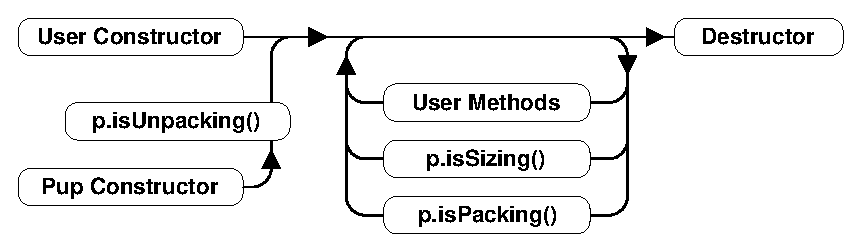
\includegraphics[width=6.0in]{fig/pup}
\end{center}
\caption{Life cycle of an object with a pup routine.}
\label{fig:pup}
\end{figure}

The life cycle of an object with a pup routine is shown in 
Figure~\ref{fig:pup}.  As usual in \CC{}, objects are 
constructed, do some processing, and are then destroyed.

Objects can be created in one of two ways: they can
be created using a normal constructor as usual; or they
can be created using their pup constructor.  The pup constructor
for \charmpp{} array elements and \kw{PUP::able} objects
is a ``migration constructor'' that takes a single ``CkMigrateMessage *";
for other objects, such as parameter marshalled objects,
the pup constructor has no parameters.  The pup constructor
is always followed by a call to the object's pup routine in
\verb.isUnpacking. mode.

Once objects are created, they respond to regular user methods
and remote entry methods as usual.  At any time, the object 
pup routine can be called in \verb.isSizing. or \verb.isPacking.
mode.  User methods and sizing or packing pup routines can be called
repeatedly over the object lifetime.

Finally, objects are destroyed by calling their destructor
as usual.



\subsubsection{Dynamic Allocation}

\label{sec:pupdynalloc}

If your class has fields that are dynamically allocated, when unpacking
these need to be allocated (in the usual way) before you pup them.
Deallocation should be left to the class destructor as usual.

\paragraph{No allocation}

The simplest case is when there is no dynamic allocation.
\begin{alltt}
class keepsFoo : public mySuperclass \{
private:
    foo f; /* simple foo object*/
public:
    keepsFoo(void) \{ \}
    void pup(PUP::er &p) \{
      p|f; // pup f's fields (calls f.pup(p);) 
    \}
    ~keepsFoo() \{ \}
\};
\end{alltt}

\paragraph{Allocation outside pup}

The next simplest case is when we contain a class 
that is always allocated during our constructor,
and deallocated during our destructor.  Then no allocation
is needed within the pup routine.
\begin{alltt}
class keepsHeapFoo : public mySuperclass \{
private:
    foo *f; /*Heap-allocated foo object*/
public:
    keepsHeapFoo(void) \{
      f=new foo;
    \}
    void pup(PUP::er &p) \{
      p|*f; // pup f's fields (calls f->pup(p))
    \}
    ~keepsHeapFoo() \{delete f;\}
\};
\end{alltt}

\paragraph{Allocation during pup}

If we need values obtained during the pup routine
before we can allocate the class, we must 
allocate the class inside the pup routine.
Be sure to protect the allocation with ``if (p.isUnpacking())''.
\begin{alltt}
class keepsOneFoo : public mySuperclass \{
private:
    foo *f; /*Heap-allocated foo object*/
public:
    keepsOneFoo(...) \{f=new foo(...);\}
    keepsOneFoo() \{f=NULL;\} /* pup constructor */
    void pup(PUP::er &p) \{
      ...
      if (p.isUnpacking()) /* must allocate foo now */
         f=new foo(...);
      p|*f;//pup f's fields
    \}
    ~keepsOneFoo() \{delete f;\}
\};
\end{alltt}

\paragraph{Allocatable array}

For example, if we keep an array of doubles,
we need to know how many doubles there are 
before we can allocate the array.  Hence we must
first pup the array length, do our allocation,
and then pup the array data.  We could allocate memory using 
malloc/free or other allocators in exactly the same way.
\begin{alltt}
class keepsDoubles : public mySuperclass \{
private:
    int n;
    double *arr;/*new'd array of n doubles*/
public:
    keepsDoubles(int n_) \{
      n=n_;
      arr=new double[n];
    \}
    keepsDoubles() \{ \} 
    
    void pup(PUP::er &p) \{
      p|n;//pup the array length n
      if (p.isUnpacking())  arr=new double[n];
      PUParray(p,arr,n); //pup data in the array
    \}
    
    ~keepsDoubles() \{delete[] arr;\}
\};
\end{alltt}

\paragraph{NULL object pointer}

If our allocated object may be NULL, our allocation
becomes much more complicated.  We must first check
and pup a flag to indicate whether the object exists, 
then depending on the flag, pup the object.
\begin{alltt}
class keepsNullFoo : public mySuperclass \{
private:
    foo *f; /*Heap-allocated foo object, or NULL*/
public:
    keepsNullFoo(...) \{ if (...) f=new foo(...);\}
    keepsNullFoo() \{f=NULL;\}
    void pup(PUP::er &p) \{
      int has_f=(f!=NULL);
      p|has_f;
      if (has_f) {
        if (p.isUnpacking()) f=new foo;
        p|*f;
      } else {
        f=NULL;
      }
    \}
    ~keepsNullFoo() \{delete f;\}
\};
\end{alltt}

This sort of code is normally much longer and more
error-prone if split into the various packing/unpacking cases.

\paragraph{Array of classes}

An array of actual classes can be treated exactly the same way
as an array of basic types.  PUParray will pup each 
element of the array properly, calling the appropriate \verb.operator|..
\begin{alltt}
class keepsFoos : public mySuperclass \{
private:
    int n;
    foo *arr;/*new'd array of n foos*/
public:
    keepsFoos(int n_) \{
      n=n_;
      arr=new foo[n];
    \}
    keepsFoos() \{ arr=NULL; \} 
    
    void pup(PUP::er &p) \{
      p|n;//pup the array length n
      if (p.isUnpacking())  arr=new foo[n];
      PUParray(p,arr,n); //pup each foo in the array
    \}
    
    ~keepsFoos() \{delete[] arr;\}
\};
\end{alltt}


\paragraph{Array of pointers to classes}

An array of pointers to classes must handle each element
separately, since the PUParray routine does not work with 
pointers.  An ``allocate'' routine to set up the array
could simplify this code.  More ambitious is to construct
a ``smart pointer'' class that includes a pup routine.
\begin{alltt}
class keepsFooPtrs : public mySuperclass \{
private:
    int n;
    foo **arr;/*new'd array of n pointer-to-foos*/
public:
    keepsFooPtrs(int n_) \{
      n=n_;
      arr=new foo*[n]; // allocate array
      for (int i=0;i<n;i++) arr[i]=new foo(...); // allocate i'th foo
    \}
    keepsFooPtrs() \{ arr=NULL; \} 
    
    void pup(PUP::er &p) \{
      p|n;//pup the array length n
      if (p.isUnpacking()) arr=new foo*[n]; // allocate array
      for (int i=0;i<n;i++) \{
        if (p.isUnpacking()) arr[i]=new foo(...); // allocate i'th foo
        p|*arr[i];  //pup the i'th foo
      \}
    \}
    
    ~keepsFooPtrs() \{
       for (int i=0;i<n;i++) delete arr[i];
       delete[] arr;
     \}
\};
\end{alltt}

Note that this will not properly handle the case where
some elements of the array are actually subclasses of foo,
with virtual methods.  The PUP::able framework described
in the next section can be helpful in this case.


\subsubsection{Subclass allocation via PUP::able}

\label{sec:pup::able}
If the class \uw{foo} above might have been a subclass, instead of
simply using \uw{new foo} above we would have had to allocate 
an object of the appropriate subclass.  Since determining the
proper subclass and calling the appropriate constructor yourself can be 
difficult, the PUP framework provides a scheme for automatically
determining and dynamically allocating subobjects of the appropriate type.

Your superclass must inherit from \kw{PUP::able}, which provides 
the basic machinery used to move the class.  
A concrete superclass and all its concrete subclasses require these
four features:

\begin{itemize}
\item A line declaring \kw{PUPable \uw{className};} in the .ci file.
This registers the class's constructor.

\item A call to the macro \kw{PUPable\_decl(\uw{className})} in the
class's declaration, in the header file.  This adds a virtual 
method to your class to allow \kw{PUP::able} to determine your class's type.

\item A migration constructor---a constructor that takes \kw{CkMigrateMessage *}.
This is used to create the new object on the receive side, immediately
before calling the new object's \kw{pup} routine.

\item A working, virtual \kw{pup} method.  You can omit this if your
class has no data that needs to be packed.
\end{itemize}

An abstract superclass---a superclass that will never actually be 
packed---only needs to inherit from \kw{PUP::able} and include a 
\kw{PUPable\_abstract(\uw{className})} macro in their body.  For
these abstract classes, the 
.ci file, \kw{PUPable\_decl} macro, and constructor are not needed.

For example, if \uw{parent} is a concrete superclass and \uw{child} its
subclass,

\begin{alltt}
//In the .ci file:
   PUPable parent;
   PUPable child; //Could also have said ``PUPable parent, child;''

//In the .h file:
class parent : public PUP::able \{
    ... data members ...
public:
    ... other methods ...
    parent() \{...\}
    
    //PUP::able support: decl, migration constructor, and pup
    PUPable\_decl(parent);  
    parent(CkMigrateMessage *m) : PUP::able(m) \{\}
    virtual void pup(PUP::er &p) \{
        PUP::able::pup(p);//Call base class
        ... pup data members as usual ...
    \}  
\};
class child : public parent \{
    ... more data members ...
public:    ... more methods, possibly virtual ...
    child() \{...\}
    
    //PUP::able support: decl, migration constructor, and pup
    PUPable\_decl(child);  
    child(CkMigrateMessage *m) : parent(m) \{\}
    virtual void pup(PUP::er &p) \{
        parent::pup(p);//Call base class
        ... pup child's data members as usual ...
    \}  
\};

\end{alltt}

With these declarations, then, we can automatically 
allocate and pup a pointer to a parent or child
using the vertical bar \kw{PUP::er} syntax, which on the receive
side will create a new object of the appropriate type:

\begin{alltt}
class keepsParent \{
    parent *obj; //May actually point to a child class (or be NULL)
public:
    ...
    ~keepsParent() \{
        delete obj;
    \}
    void pup(PUP::er &p) 
    \{
        p|obj;
    \}
\};
PUPmarshall(keepsParent);
\end{alltt}

This will properly pack, allocate, and unpack obj whether
it is actually a parent or child object.  The child class 
can use all the usual \CC\ features, such as virtual functions
and extra private data.

If obj is NULL when packed, it will be restored to NULL when unpacked.
For example, if the nodes of a binary tree are \kw{PUP::able},
one may write a recursive pup routine for the tree quite easily:

\begin{alltt}
// In the .ci file:
    PUPable treeNode;

// In the .h file
class treeNode : public PUP::able \{
    treeNode *left;//Left subtree
    treeNode *right;//Right subtree
    ... other fields ...
public:
    treeNode(treeNode *l=NULL, treeNode *r=NULL);
    ~treeNode() \{delete left; delete right;\}
    
    // The usual PUP::able support:
    PUPable\_decl(treeNode);
    treeNode(CkMigrateMessage *m) : PUP::able(m) \{ left=right=NULL; \}
    void pup(PUP::er &p) \{
        PUP::able::pup(p);//Call base class
        p|left;
        p|right;
        ... pup other fields as usual ...
    \}
\};
\end{alltt}

This same implementation will also work properly even if the tree's
internal nodes are actually subclasses of treeNode.

You may prefer to use the macros \kw{PUPable\_def(\uw{className})}
and \kw{PUPable\_reg(\uw{className})} rather than using \kw{PUPable}
in the .ci file.  \kw{PUPable\_def} provides routine definitions used
by the \kw{PUP::able} machinery, and should be included in exactly one
source file at file scope.  \kw{PUPable\_reg} registers this class
with the runtime system, and should be executed exactly once per node 
during program startup.

Finally, a \kw{PUP::able} superclass like \uw{parent} above 
must normally be passed around via a pointer or reference, because the object
might actually be some subclass like \uw{child}.  Because
pointers and references cannot be passed across processors,
for parameter marshalling you must use the special templated 
smart pointer classes \kw{CkPointer} and \kw{CkReference},
which only need to be listed in the .ci file.

A \kw{CkReference} is a read-only reference to a \kw{PUP::able} object---it
is only valid for the duration of the method call.  A \kw{CkPointer}
transfers ownership of the unmarshalled \kw{PUP::able} to the method, so the 
pointer can be kept and the object used indefinitely.  

For example, if the entry method \uw{bar} needs a \kw{PUP::able} \uw{parent}
object for in-call processing, you would use a \kw{CkReference} like this:

\begin{alltt}
// In the .ci file:
    entry void barRef(int x,CkReference<parent> p);

// In the .h file:
    void barRef(int x,parent &p) \{
      // can use p here, but only during this method invocation
    \}
\end{alltt}

If the entry method needs to keep its parameter, use a \kw{CkPointer} like this:
\begin{alltt}
// In the .ci file:
    entry void barPtr(int x,CkPointer<parent> p);

// In the .h file:
    void barPtr(int x,parent *p) \{
      // can keep this pointer indefinitely, but must eventually delete it
    \}
\end{alltt}

Both \kw{CkReference} and \kw{CkPointer} are read-only from the send 
side---unlike messages, which are consumed when sent, the same object 
can be passed to several parameter marshalled entry methods.
In the example above, we could do:

\begin{alltt}
   parent *p=new child;
   someProxy.barRef(x,*p);
   someProxy.barPtr(x,p); // Makes a copy of p
   delete p; // We allocated p, so we destroy it.
\end{alltt}


\subsubsection{C and Fortran bindings}

C and Fortran programmers can use a limited subset of the
\kw{PUP::er} capability.  The routines all take a 
handle named \kw{pup\_er}.  The routines 
have the prototype:
\begin{alltt}
void pup\_\kw{type}(pup\_er p,\kw{type} *val);
void pup\_\kw{type}s(pup\_er p,\kw{type} *vals,int nVals);
\end{alltt}
The first call is for use with a single element;
the second call is for use with an array.
The supported types are char, short, int, long,
uchar, ushort, uint, ulong, float, and double,
which all have the usual C meanings.

A byte-packing routine
\begin{alltt}
void pup\_bytes(pup\_er p,void *data,int nBytes);
\end{alltt}
is also provided, but its use is discouraged
for cross-platform puping.

\kw{pup\_isSizing}, \kw{pup\_isPacking}, \kw{pup\_isUnpacking},
and \kw{pup\_isDeleting} calls are also available.
Since C and Fortran have no destructors, you should 
actually deallocate all data when passed a deleting \kw{pup\_er}.

C and Fortran users cannot use \kw{PUP::able} objects, 
seeking, or write custom \kw{PUP::er}s. Using the \CC\
interface is recommended.



\subsubsection{Common PUP::ers}

The most common \kw{PUP::er}s used are \kw{PUP::sizer},
\kw{PUP::toMem}, and \kw{PUP::fromMem}.  These are sizing,
packing, and unpacking \kw{PUP::er}s, respectively.

\kw{PUP::sizer} simply sums up the sizes of the native
binary representation of the objects it is passed.
\kw{PUP::toMem} copies the binary representation of the
objects passed into a preallocated contiguous memory buffer.
\kw{PUP::fromMem} copies binary data from a contiguous memory
buffer into the objects passed.  All three support the
\kw{size} method, which returns the number of bytes used
by the objects seen so far.

Other common \kw{PUP::er}s are \kw{PUP::toDisk}, 
\kw{PUP::fromDisk}, and \kw{PUP::xlater}.  The first
two are simple filesystem variants of the \kw{PUP::toMem} 
and \kw{PUP::fromMem} classes; \kw{PUP::xlater} translates
binary data from an unpacking PUP::er into the machine's
native binary format, based on a \kw{machineInfo} structure
that describes the format used by the source machine.


\subsubsection{PUP::seekBlock}

It may rarely occur that you require items to be unpacked
in a different order than they are packed.  That is, you
want a seek capability.  \kw{PUP::er}s support a limited 
form of seeking.

To begin a seek block, create a \kw{PUP::seekBlock} object
with your current PUP::er and the number of ``sections'' to 
create.  Seek to a (0-based) section number
with the seek method, and end the seeking with the endBlock method.
For example, if we have two objects A and B, where A's pup
depends on and affects some object B, we can pup the two with:

\begin{alltt}
void pupAB(PUP::er &p)
\{
  ... other fields ...
  PUP::seekBlock s(p,2); //2 seek sections
  if (p.isUnpacking()) 
  \{//In this case, pup B first
    s.seek(1);
    B.pup(p);
  \}
  s.seek(0);
  A.pup(p,B);
  
  if (!p.isUnpacking()) 
  \{//In this case, pup B last
    s.seek(1);
    B.pup(p);
  \}
  s.endBlock(); //End of seeking block
  ... other fields ...
\};
\end{alltt}

Note that without the seek block, A's fields would be unpacked
over B's memory, with disasterous consequences.
The packing or sizing path must traverse the seek sections
in numerical order; the unpack path may traverse them in any
order.  There is currently a small fixed limit of 3 on the 
maximum number of seek sections.


\subsubsection{Writing a PUP::er}

System-level programmers may occasionally find it useful to define
their own \kw{PUP::er} objects.  The system \kw{PUP::er} class is 
an abstract base class that funnels all incoming pup requests
to a single subroutine:

\begin{alltt}
    virtual void bytes(void *p,int n,size\_t itemSize,dataType t);
\end{alltt}

The parameters are, in order, the field address, the number of items,
the size of each item, and the type of the items. The \kw{PUP::er}
is allowed to use these fields in any way.  However, an isSizing
or isPacking PUP::er may not modify the referenced user data; 
while an isUnpacking PUP::er may not read the original values of 
the user data.  If your PUP::er is not clearly packing (saving values
to some format) or unpacking (restoring values), declare it as 
sizing \kw{PUP::er}.





\chapter{Load Balancing}
\label{loadbalancing}
  Load balancing in \charmpp{} is enabled by its ability to place, or
migrate, chares or chare array elements.  Typical application usage to
exploit this feature will construct many more chares than processors, and
enable their runtime migration.

Iterative applications, which are commonplace in physical simulations,
are the most suitable target for \charmpp{}'s measurement based load
balancing techniques.  Such applications may contain a series of
time-steps, and/or iterative solvers that run to convergence. For such
computations, typically, the heuristic principle that we call
``principle of persistence'' holds: the computational loads and
communication patterns between objects (chares) tend to persist over
multiple iterations, even in dynamic applications. In such cases,
the recent past is a good predictor of the near future. Measurement-based
chare migration strategies are useful in this context. Currently these
apply to chare-array elements, but they may be extended to chares in
the future.

For applications without such iterative structure, or with iterative
structure, but without predictability (i.e. where the principle of
persistence does not apply), Charm++ supports ``seed balancers'' that
move ``seeds'' for new chares among processors (possibly repeatedly)
to achieve load balance. These strategies are currently available for
both chares and chare-arrays.  Seed balancers were the original load
balancers provided in Charm since the late 80's. They are extremely
useful for state-space search applications, and are also useful in
other computations, as well as in conjunction with migration
strategies.

For iterative computations when there is a correlation between iterations/steps,
but either it is not strong, or the machine environment is not predictable
(due to noise from OS interrupts on small time steps, or time-shared desktop
machines), one can use a combination of the two kinds of strategies. The
baseline load balancing is provided by migration strategies, but in each
iteration one also spawns off work in the form of chares that can run on any
processor. The seed balancer will handle such work as it arises.

Examples are in \examplerefdir{load\_balancing} and
\testrefdir{load\_balancing}

\section{Measurement-based Object Migration Strategies}
\label{lbFramework}
\label{migrationlb}

In \charmpp{}, objects (except groups, nodegroups) can migrate from 
processor to processor at runtime. Object migration can potentially 
improve the performance of the parallel program by migrating objects from 
overloaded processors to underloaded ones. 

%However, it is not
%trivial to decide which objects to move and where to move them in 
%order to achieve load balance in a fashion without the knowledge about the 
%application. The strategy used in \charmpp{} load balancing framework
%is a measurement-based one.

 \charmpp{} implements a generic, measurement-based load balancing framework
which automatically instruments all \charmpp{} objects, collects computation
load and communication structure during execution and stores them into a
\kw{load balancing database}. \charmpp{} then provides a collection of \kw{load
balancing strategies} whose job it is to decide on a new mapping of objects to
processors based on the information from the database.  Such measurement based
strategies are efficient when we can reasonably assume that objects in a 
\charmpp{} application tend to exhibit temporal correlation in their
computation and communication patterns, i.e. future can be to some extent
predicted using the historical measurement data, allowing effective
measurement-based load balancing without application-specific knowledge.

Two key terms in the \charmpp{} load balancing framework are:
\begin{itemize}
%
\item \kw{Load balancing database} provides the interface of almost all load
balancing calls. On each processor, it stores the load balancing instrumented
data and coordinates the load balancing manager and balancer. It is implemented
as a Chare Group called \kw{LBDatabase}.
%
\item \kw{Load balancer or strategy} takes the load balancing database and
produces the new mapping of the objects. In \charmpp{}, it is implemented as
Chare Group inherited from BaseLB. Three kinds of schemes are implemented: (a)
centralized load balancers, (b) fully distributed load balancers and (c)
hierarchical load balancers.
%
\end{itemize}

\section{Available Load Balancing Strategies}
\label{lbStrategy}

Load balancing can be performed in either a centralized, a fully distributed,
or an hierarchical fashion.

In centralized approaches, the entire machine's load and communication
structure are accumulated to a single point, typically processor 0, followed by
a decision making process to determine the new distribution of \charmpp
objects. Centralized load balancing requires synchronization which may incur an
overhead and delay. However, due to the fact that the decision process has a
high degree of the knowledge about the entire platform, it tends to be more
accurate.

In distributed approaches, load data is only exchanged among 
neighboring processors. There is no global synchronization. However,
they will not, in general, provide an immediate restoration for load balance -
the process is iterated until the load balance can be achieved.

In hierarchical approaches, processors are divided into independent autonomous
sets of processor groups and these groups are organized in hierarchies,
thereby decentralizing the load balancing task. Different strategies can be
used to balance the load on processors inside each processor group, and
processors across groups in a hierarchical fashion.

Listed below are some of the available non-trivial centralized load balancers
and their brief descriptions:
\begin{itemize}
\item {\bf RandCentLB}:   Randomly assigns objects to processors;
%\item {\bf RecBisectBfLB}:        Recursively partition with Breadth first enumeration;
\item {\bf MetisLB}:      Uses METIS\texttrademark\hspace{0mm} to partitioning object communication graph.
\item {\bf GreedyLB}:   Uses a greedy algorithm that always assigns the heaviest object to the least loaded processor.
\item {\bf GreedyCommLB}:  Extends the greedy algorithm to take the communication graph into account.
\item {\bf TopoCentLB}:    Extends the greedy algorithm to take processor topology into account.
\item {\bf RefineLB}:     Moves objects away from the most overloaded processors to reach average, limits the number of objects migrated.
\item {\bf RefineSwapLB}:     Moves objects away from the most overloaded processors
to reach average. In case it cannot migrate an object from an overloaded
processor to an underloaded processor, it swaps objects to reduce the load on
the overloaded processor. This strategy limits the number of objects migrated.
\item {\bf RefineCommLB}:     Same idea as in RefineLB, but takes communication into account.
\item {\bf RefineTopoLB}:       Same idea as in RefineLB, but takes processor topology into account.
\item {\bf BlockLB}: This strategy does a blocked distribution of objects to
processors.
\item {\bf ComboCentLB}:  A special load balancer that can be used to combine any number of centralized load balancers mentioned above.
\end{itemize}

Listed below are the distributed load balancers:
\begin{itemize}
\item {\bf NeighborLB}:   A neighborhood load balancer in which each processor tries to average out its load only among its neighbors.
\item {\bf WSLB}:   A load balancer for workstation clusters, which can detect load changes on desktops (and other timeshared processors) and adjust load without interfering with other's use of the desktop.
\item {\bf DistributedLB}: A load balancer which uses partial information about
underloaded and overloaded processors in the system to do probabilistic transfer
of load. This is a refinement based strategy.
\end{itemize}

An example of a hierarchical strategy can be found in:
\begin{itemize}
\item {\bf HybridLB}: This calls GreedyLB at the lower level and RefineLB at
the root.
\end{itemize}

Users can choose any load balancing strategy they think is appropriate for their
application. The compiler and runtime options are described in
section~\ref{lbOption}.

%In some cases, one may need to create and invoke multiple load balancing
%strategies/algorithms at the different phases. \charmpp{} now supports
%multiple load balancers created at runtime. For example, one can use 
%an aggressive load balancer such as GreedyRefLB in the first load balancing
%step, and use RefineLB for the later load balancing steps.

\section{Load Balancing Chare Arrays}
\label{lbarray}

The load balancing framework is well integrated with chare array implementation
-- when a chare array is created, it automatically registers its elements with
the load balancing framework. The instrumentation of compute time (WALL/CPU
time) and communication pattern is done automatically and APIs are provided
for users to trigger the load balancing.  To use the load balancer, you must
make your array elements migratable (see migration section above) and choose a
\kw{load balancing strategy} (see the section \ref{lbStrategy} for a
description of available load balancing strategies).

There are three different ways to use load balancing for chare arrays to meet
different needs of the applications. These methods are different in how and
when a load balancing phase starts. The three methods are: {\bf periodic load
balancing mode}, {\bf at sync mode} and {\bf manual mode}.

In {\em periodic load balancing mode}, a user specifies only how often
load balancing is to occur, using +LBPeriod runtime option to specify
the time interval.

In {\em at sync mode}, the application invokes the load balancer
explicitly at appropriate (generally at a pre-existing synchronization
boundary) to trigger load balancing by inserting a function call
(AtSync) in the application source code.

In the prior two load balancing modes, users do not need to worry
about how to start load balancing.  However, in one scenario, those
automatic load balancers will fail to work - when array elements are
created by dynamic insertion.  This is because the above two load
balancing modes require an application to have fixed the number of
objects at the time of load balancing.  The array manager needs to
maintain a head count of local array elements for the local barrier.
In this case, the application must use the {\em manual mode} to
trigger load balancer.

The detailed APIs of these three methods are described as follows:
%
\begin{enumerate}
%
\item {\bf Periodical load balancing mode}: In the default setting, load
balancing happens whenever the array elements are ready, with an interval of 1
second. It is desirable for the application to set a larger interval using
+LBPeriod runtime option. For example ``+LBPeriod 5.0'' can be used to start load
balancing roughly every 5 seconds. By default, array elements may be asked to
migrate at any time, provided that they are not in the middle of executing an
entry method. The array element's variable \kw{usesAtSync} being false
attributes to this default behavior.
%
\item {\bf At sync mode}: Using this method, elements can be migrated only at
certain points in the execution when the application invokes \kw{AtSync()}. In order to use the at
sync mode, one should set \kw{usesAtSync} to true in the array element
constructor.  When an element is ready to migrate, call
\kw{AtSync()}~\footnote{AtSync() is a member function of class ArrayElement}.
When all local elements call \kw{AtSync}, the load balancer is triggered.  Once
all migrations are completed, the load balancer calls the virtual function
\kw{ArrayElement::ResumeFromSync()} on each of the array elements. This
function can be redefined in the application.

Note that the minimum time for \kw{AtSync()} load balancing to occur
is controlled by the LBPeriod.  Unusually high frequency load
balancing (more frequent than 500ms) will perform better if this value
is set via +LBPeriod or \kw{SetLBPeriod()} to a number shorter than your load
balancing interval.

Note that {\em AtSync()} is not a blocking call, it just gives a hint to load
balancing that it is time for load balancing. During the time between {\em
AtSync} and {\em ResumeFromSync}, the object may be migrated. One can choose
to let objects continue working with incoming messages, however keep in mind
the object may suddenly show up in another processor and make sure no
operations that could possibly prevent migration be performed. This is 
the automatic way of doing load balancing where the application does not need to define ResumeFromSync().

The more commonly used approach is to force the object to be idle until load
balancing finishes. The user places an AtSync call at the end of some iteration
and when all elements reach that call load balancing is triggered. The objects
can start executing again when \kw{ResumeFromSync()} is called. In this case,
the user redefines ResumeFromSync() to trigger the next iteration of the
application. This manual way of using the at sync mode results in a barrier at
load balancing (see example here~\ref{lbexample}).
%
\item {\bf Manual mode}: The load balancer can be programmed to be started
manually. To switch to the manual mode, the application calls {\em TurnManualLBOn()}
on every processor to prevent the load balancer from starting automatically. {\em
TurnManualLBOn()} should be called as early as possible in the program. It
could be called at the initialization part of the program, for example from a
global variable constructor, or in an initproc call (Section~\ref{initproc}).  It can also be
called in the constructor of a static array or before the {\em
doneInserting} call for a dynamic array.  It can be called multiple times on
one processor, but only the last one takes effect.

The function call {\em CkStartLB()} starts load balancing immediately. This call
should be made at only one place on only one processor. This function is
not blocking, the object will continue to process messages and the load
balancing, when triggered, happens in the background.

{\em TurnManualLBOff()} turns off manual load balancing and switches back to
the automatic load balancing mode.
%
\end{enumerate}

\section{Migrating objects}
\label{lbmigobj}

Load balancers migrate objects automatically.
For an array element to migrate, user can refer to Section~\ref{arraymigratable}
for how to write a ``pup'' for an array element.

In general one needs to pack the whole snapshot of the member data in an 
array element in the pup subroutine. This is because the migration of
the object may happen at any time. In certain load balancing schemes where
 the user explicitly controls when load balancing occurs, the user may choose
to pack only a part of the data and may skip temporary data.

An array element can migrate by calling the \kw{migrateMe}(\uw{destination
processor}) member function-- this call must be the last action
in an element entry method.  The system can also migrate array elements
for load balancing (see the section~\ref{lbarray}).

To migrate your array element to another processor, the \charmpp{}
runtime will:

\begin{itemize}
\item Call your \kw{ckAboutToMigrate} method
\item Call your \uw{pup} method with a sizing \kw{PUP::er} to determine how 
big a message it needs to hold your element.
\item Call your \uw{pup} method again with a packing \kw{PUP::er} to pack 
your element into a message.
\item Call your element's destructor (deleting the old copy).
\item Send the message (containing your element) across the network.
\item Call your element's migration constructor on the new processor.
\item Call your \uw{pup} method on with an unpacking \kw{PUP::er} to unpack 
the element.
\item Call your \kw{ckJustMigrated} method
\end{itemize}

Migration constructors, then, are normally empty-- all the unpacking
and allocation of the data items is done in the element's \uw{pup} routine.
Deallocation is done in the element destructor as usual.


\section{Other utility functions}

There are several utility functions that can be called in applications to
configure the load balancer, etc. These functions are:

\begin{itemize}
\item {\bf LBTurnInstrumentOn()} and {\bf LBTurnInstrumentOff()}: are plain C
      functions to control the load balancing statistics instrumentation
      on or off on the calling processor. No implicit broadcast or 
      synchronization exists in these functions.
      Fortran interface: {\bf FLBTURNINSTRUMENTON()} and {\bf FLBTURNINSTRUMENTOFF()}.
\item {\bf setMigratable(bool migratable)}: is a member function of array
      element. This function can be called 
      in an array element constructor to tell the load balancer whether this object
      is migratable or not\footnote{Currently not all load balancers 
      recognize this setting though.}.
\item {\bf LBSetPeriod(double s)}: this function can be called
      anywhere (even in Charm++ initnodes or initprocs) to specify 
      the load balancing period time in seconds. 
      It tells load balancer not to start next 
      load balancing in less than $s$ seconds. This can be used to prevent 
      load balancing from occurring too often in 
      {\em automatic without sync mode}. Here is how to use it:
      \begin{alltt}
// if used in an array element
LBDatabase *lbdb = getLBDB();
lbdb->SetLBPeriod(5.0);

// if used outside of an array element
LBSetPeriod(5.0);
\end{alltt}
      Alternatively, one can specify +LBPeriod \{seconds\} at command line.
\end{itemize}

\section{Compiler and runtime options to use load balancing module}
\label{lbOption}

Load balancing strategies are implemented as libraries in \charmpp{}. This
allows programmers to easily experiment with different existing strategies 
by simply linking a pool of strategy modules and choosing
one to use at runtime via a command line option.

{\bf Note:} linking a load balancing module is different from activating it:
\begin{itemize}
\item link an LB module: is to link a Load Balancer module(library) at 
   compile time. You can link against multiple LB libraries as candidates.
\item activate an LB: is to actually ask the runtime to create an LB strategy and 
   start it. You can only activate load balancers that have been linked at
   compile time.
\end{itemize}


Below are the descriptions about the compiler and runtime options:

\begin{enumerate}
\item {\bf compile time options:}

\begin{itemize}
\item {\em -module NeighborLB -module GreedyCommLB ...}  \\
  links the modules NeighborLB, GreedyCommLB etc into an application, but these
load balancers will remain inactive at execution time unless overridden by other
runtime options.
\item {\em -module CommonLBs} \\
  links a special module CommonLBs which includes some commonly used \charmpp{}
built-in load balancers. The commonly used load balancers include {\tt
DummyLB, GreedyLB, CommLB, RandCentLB, RefineLB, RefineCommLB, RotateLB, DistributedLB, HybridLB, ComboCentLB, RefineSwapLB, NeighborLB, OrbLB, BlockLB, GreedyCommLB}
\item {\em -balancer GreedyCommLB} \\
  links the load balancer GreedyCommLB and invokes it at runtime.
\item {\em -balancer GreedyCommLB -balancer RefineLB} \\
  invokes GreedyCommLB at the first load balancing step and RefineLB in all
subsequent load balancing steps.
\item {\em -balancer ComboCentLB:GreedyLB,RefineLB}  \\
  You can create a new combination load balancer made of multiple
load balancers. In the above example, GreedyLB and RefineLB strategies are
applied one after the other in each load balancing step.
\end{itemize}

The list of existing load balancers is given in Section
\ref{lbStrategy}. Note: you can have multiple -module *LB options. LB
modules are linked into a program, but they are not activated
automatically at runtime.  Using -balancer A at compile time will
activate load balancer A automatically at runtime.  Having -balancer A
implies -module A, so you don't have to write -module A again,
although that is not invalid.  Using CommonLBs is a convenient way to
link against the commonly used existing load balancers.  

Two families of load balancers based on external partitioning libraries require 3rd party software:

METIS can be downloaded from:
\url{http://glaros.dtc.umn.edu/gkhome/metis/metis/download}

SCOTCH can be downloaded from:
\url{http://www.labri.fr/perso/pelegrin/scotch/}

Use the {\em --with-metis=/path/to/lib, or --incdir and --libdir} build time option to add your installation of any third party libraries you wish to use to the \charmpp{} search paths.  

\item {\bf Building individual load balancers}

Load balancers can be built individually by changing the current working directory to the {\em tmp} subdirectory of your build and making them by name.

\begin{alltt}
 cd netlrts-linux-x86\_64/tmp
 make PhasebyArrayLB
\end{alltt}

Or, if the METIS library has been installed, METIS based balancers can be built like so:
\begin{alltt}
 cd netlrts-linux-x86\_64/tmp
 make MetisLB
\end{alltt}

\item {\bf Write and use your own load balancer}

Refer Section~\ref{lbWriteNewLB} for writing a new load balancer. Compile it in
the form of library and name it {\em libmoduleFooLB.a} where {\em FooLB} is the
new load balancer. Add the path to the library and link the load balancer into
an application using {\em -module FooLB}. 

You can create a library by modifying the Makefile in the following way. This
will create {\em libmoduleFooLB.a}.
\begin{alltt}
libmoduleFooLB.a: FooLB.o
  $(CHARMC) -o libmoduleFooLB.a FooLB.o
\end{alltt}

To include this balancer in your application, the Makefile can be changed in the
following way
\begin{alltt}
$(TARGET): $(OBJECTS)
  $(CHARMC) -o $(TARGET) -L/path-to-the-lib $(OBJS) -module FooLB 
\end{alltt}


\item {\bf runtime options:}

Runtime balancer selection options are similar to the compile time
options as described above, but they can be used to override those
compile time options.

\begin{itemize}
\item {\em +balancer help} \\
  displays all available balancers that have been linked in.
\item {\em +balancer GreedyCommLB} \\
  invokes GreedyCommLB
\item {\em +balancer GreedyCommLB +balancer RefineLB} \\
  invokes GreedyCommLB at the first load balancing step and RefineLB in all
subsequent load balancing steps.
\item {\em +balancer ComboCentLB:GreedyLB,RefineLB}  \\
  same as the example in the -balancer compile time option.
\end{itemize}

Note: +balancer option works only if you have already linked the corresponding 
load balancers module at compile time. 
Giving +balancer with a wrong LB name will result in a runtime error.
When you have used -balancer A as compile time option, you do not need to use 
+balancer A again to activate it at runtime. However, you can 
use +balancer B to override the compile time option and choose to
activate B instead of A.

\item {\bf Handling the case that no load balancer is activated by users}

When no balancer is linked by users, 
but the program counts on a load balancer because it used {\em AtSync()}
and expect {\em ResumeFromSync()} to be called to continue,
a special load balancer called {\em NullLB} will be 
automatically created to run the program.
This default load balancer calls {\em ResumeFromSync()} after {\em AtSync()}. 
It keeps a program from hanging after calling {\em AtSync()}.
{\em NullLB} will be suppressed if another load balancer is created.

\item {\bf Other useful runtime options}

There are a few other runtime options for load balancing that may be useful:

\begin{itemize}
\item {\em +LBDebug \{verbose level\}} \\
     \{verbose level\} can be any positive integer number. 0 is to turn off the verbose. 
     This option asks load balancer to output load balancing information to stdout.
     The bigger the verbose level is, the more verbose the output is.
\item {\em +LBPeriod \{seconds\}} \\
     \{Seconds\} can be any float number. This option sets the minimum period time in 
seconds between two consecutive load balancing steps. The default value is 
1 second. That is to say that a load balancing step will not happen until
1 second after the last load balancing step.
\item {\em +LBSameCpus} \\
     This option simply tells load balancer that all processors are of same speed.
     The load balancer will then skip the measurement of CPU speed at runtime. This is the default.
\item {\em +LBTestPESpeed} \\
     This option tells the load balancer to test the speed of all processors at runtime.
     The load balancer may use this measurement to perform speed-aware load balancing.
\item {\em +LBObjOnly} \\
     This tells load balancer to ignore processor background load when making migration decisions.
\item {\em +LBSyncResume} \\
     After load balancing step, normally a processor can resume computation 
once all objects are received on that processor, even when other processors
are still working on migrations.  If this turns out to be a problem, 
that is when some processors start working on computation while the other 
processors are still busy migrating objects, then this option can be used to force 
a global barrier on all processors to make sure that processors can only resume 
computation after migrations are completed on all processors.
\item {\em +LBOff} \\
     This option turns off load balancing instrumentation 
     of both CPU and communication usage at startup time. 
\item {\em +LBCommOff} \\
     This option turns off load balancing instrumentation of communication at startup time. 
     The instrument of CPU usage is left on.
\end{itemize}

\end{enumerate}

\section{Seed load balancers - load balancing Chares at creation time}
\label{seedlb}

Seed load balancing involves the movement of object creation messages, or
"seeds", to create a balance of work across a set of processors. 
This seed load balancing scheme is used to balance chares  at creation time.
After the chare constructor is executed on a processor, the seed balancer does not
migrate it.
%the seed load balancer. The measurement based load balancer described in
%previous subsection perform the task of moving chares during work to achieve
%load balance.
Depending on the movement strategy, several seed load balancers are available now.
Examples can be found \examplerefdir{NQueen}.
\begin{enumerate}
\item {\em random}\\  
 A strategy that places seeds randomly when they are created and does
no movement of seeds thereafter. This is used as the default seed 
load balancer.
\item {\em neighbor}\\  
 A strategy which imposes a virtual topology on the processors,
 load exchange happens among neighbors only. The overloaded processors
 initiate the load balancing and send work to its neighbors
 when it becomes overloaded. The default topology is mesh2D, one can use
 command line option to choose other topology such as ring, mesh3D and 
 dense graph.
\item {\em spray}\\  
 A strategy which imposes a spanning tree organization on the processors,
 results in communication via global reduction among all processors 
 to compute global average load via periodic reduction. 
 It uses averaging of loads to determine how seeds should be
distributed.
\item  {\em workstealing} \\
 A strategy that the idle processor requests a random processor and steal 
 chares.
\end{enumerate}

Other strategies can also be explored by following the simple API of the 
seed load balancer.
\linebreak

\zap{
{\bf Seed load balancers for Chares:}

Seed load balancers can be directly used for load balancing Chares.
The default seed load balancer which is always linked is the random seed load balancer.
Users can choose another strategy listed above and link as a plugin
module into binary as described below.

{\bf Seed load balancers for Array Elements:}

Seed load balancers can also be used for array elements in the same way 
as they are used for individual chares.
Chare array is a collection of individual Chares in Charm++.
Since Chare Array has its internal strategy of static mapping of individual
array elements to processors using {\em CkArrayMap}~\ref{array map}~\footnote{by default it always distributed array elements to processors in Round-Robin fashion unless a different CkArrayMap is used}, 
a special CkArrayMap called {\em CldMap} must be created and passed into
array creation calls to interface with seed load balancer.

For creating an empty array and then inserting chares into it, the API is as follows:

\begin{alltt}
  CkArrayOptions opt;
  CkGroupID cldmapID = CProxy_CldMap::ckNew();
  opt.setMap(cldmapID);
  CProxy_WorkUnit arr = CProxy_WorkUnit::ckNew(param, opt); 
  for (int i=0; i<numChares; i++) 
    arr[i].insert(param);
\end{alltt}

For initially populating the array with chares at time of creation the API is as follows:
\begin{alltt}
  CkArrayOptions opt(numChares);
  CkGroupID cldmapID = CProxy_CldMap::ckNew();
  opt.setMap(cldmapID);
  CProxy_WorkUnit arr = CProxy_WorkUnit::ckNew(param, opt); 
\end{alltt}

The details about array creation are explained in section~\ref{advanced arrays} of the manual.

} % end zap


{\bf Compile and run time options for seed load balancers}


To choose a seed load balancer other than the default {\em rand} strategy,
use link time command line option {\bf -balance foo}. 

When using {\rm neighbor} seed load balancer, one can also specify
the virtual topology at runtime. Use {\bf +LBTopo topo}, where {\em topo}
can be one of: (a) ring, (b) mesh2d, (c) mesh3d and (d) graph.

To write a seed load balancer, name your file as {\em cldb.foo.c},
where {\em foo} is the strategy name.  Compile it in the form of library
under charm/lib, named as {\em libcldb-foo.a}, where {\em foo} is the strategy 
name used above. Now one can use {\bf -balance foo} as compile time option
to {\bf charmc} to link with the {\em foo} seed load balancer.

\section{Simple Load Balancer Usage Example - Automatic with Sync LB}
\label{lbexample}

A simple example of how to use a load balancer in sync mode in one's
application is presented below.

\begin{alltt}
/*** lbexample.ci ***/
mainmodule lbexample \{
  readonly CProxy_Main mainProxy;
  readonly int nElements;

  mainchare Main \{
    entry Main(CkArgMsg *m);
    entry void done(void);
  \};

  array [1D] LBExample \{
    entry LBExample(void);
    entry void doWork();
  \};
\};
\end{alltt}

--------------------------------------------------------------------------------

\begin{alltt}
/*** lbexample.C ***/
#include <stdio.h>
#include "lbexample.decl.h"

/*readonly*/ CProxy_Main mainProxy;
/*readonly*/ int nElements;

#define MAX_WORK_CNT 50
#define LB_INTERVAL 5

/*mainchare*/
class Main : public CBase_Main
\{
private:
  int count;
public:
  Main(CkArgMsg* m)
  \{
    /*....Initialization....*/
    mainProxy = thisProxy;
    CProxy_LBExample arr = CProxy_LBExample::ckNew(nElements);
    arr.doWork();
  \};

  void done(void)
  \{
    count++;
    if(count==nElements)\{
      CkPrintf("All done");
      CkExit();
    \}
  \};
\};

/*array [1D]*/
class LBExample : public CBase_LBExample
\{
private:
  int workcnt;
public:
  LBExample()
  \{
    workcnt=0;
    /* May initialize some variables to be used in doWork */
    //Must be set to true to make AtSync work
    usesAtSync = true;
  \}

  LBExample(CkMigrateMessage *m) \{ /* Migration constructor -- invoked when chare migrates */ \}
  
  /* Must be written for migration to succeed */
  void pup(PUP::er &p)\{
    p|workcnt;
    /* There may be some more variables used in doWork */
  \}
	
  void doWork()
  \{
    /* Do work proportional to the chare index to see the effects of LB */
    
    workcnt++;
    if(workcnt==MAX_WORK_CNT)
      mainProxy.done();
    
    if(workcnt\%LB_INTERVAL==0)
      AtSync();
    else
      doWork();
  \}
  
  void ResumeFromSync()\{
    doWork();
  \}
\};

#include "lbexample.def.h"
\end{alltt}


\chapter{Processor-Aware Chare Collections}
  \subsection{Group Objects}

A {\sl group\footnote{Originally called {\em Branch Office Chare} or 
{\em Branched Chare}}} \index{group}is a collection of chares where 
there exists \index{chare}one chare (or {\sl branch}) on each
processor.   Each branch has its own data members.  Groups have
a definition syntax similar to normal chares, except that they must
inherit from the system defined class \keyword{Group}, rather than
\keyword{Chare}.

In the interface file, we declare

\begin{tabbing}
~~~~ \=~~~~ \=~~~~ \=~~~~ \=~~~~ \=~~~~ \=~~~~ \=~~~~ \=~~~~ \=~~~~ \kill
\> \kw{group} \uw{GroupType} \{ \\
\> \>  // Interface specifications as for normal chares \\
\> \};
\end{tabbing}

In the {\tt .h} file, we define \uw{GroupType} as follows:

\begin{tabbing}
~~~~ \=~~~~ \=~~~~ \=~~~~ \=~~~~ \=~~~~ \=~~~~ \=~~~~ \=~~~~ \=~~~~ \kill
\> \kw{class} \uw{GroupType} : \kw{public Group} [,other superclasses
] \{ \\
\> \> // Data and member functions as in C++ \\
\> \> // Entry functions as for normal chares \\
\> \};
\end{tabbing}

A group is identified by a globally unique group identifier, whose type is
\kw{CkGroupID}. \index{CkGroupID}This identifier is common to all of the 
group's branches and can be obtained from the variable \keyword{thisgroup},
\index{thisgroup}which is a public local variable of the \keyword{Group} 
superclass.  For groups, \kw{thishandle} \index{thishandle} is the handle of 
the particular branch in which the function is executing: it is 
a normal chare handle.

Groups can be used to implement data-parallel operations easily.  In
addition to sending messages to a particular branch of a group, one
can broadcast messages to all branches of a group.  There can be many
instances corresponding to a group type.  Each instance has a
different group handle, and its own set of branches.

\subsubsection{Group Creation}

\noindent {\bf Chare Group Declaration}:

\noindent Given a {\tt .ci} file as follows:

\begin{verbatim}
group G {
  entry G(M1 *);
  entry void someEntry(M2 *);
};
\end{verbatim}

\noindent and the following {\tt .h} file:

\begin{verbatim}
class G : public Group {
  public:
    G(M1 *);
    void someEntry(M2 *);
};
\end{verbatim}

we can create a \index{group}group in a manner similar to a regular \index{chare}chare.  Note
the difference in how the \index{virtual handle}virtual handle is created.

\begin{verbatim}
M1 *m1 = new M1;
CProxy_G *pG = new CProxy_G(m1);
  // or
CkGroupID gid = CProxy_G::ckNew(m1);
CProxy_G g(gid);
\end{verbatim}

\subsubsection{Method Invocation on Groups}

Before sending a message to a \index{group}group via an entry
method, we need to get a proxy of that group using the group identifier (a
\index{CkGroupID}\kw{CkGroupID}). The syntax for obtaining the proxy or a proxy
pointer is:

\begin{tabbing} ~~~~ \=~~~~ \=~~~~ \=~~~~ \=~~~~ \=~~~~ \=~~~~ \=~~~~ \=~~~~
\=~~~~ \kill \> \kw{CProxy}\_\uw{groupType} {\it groupProxy}({\it groupID}); \\
\> \> or, \\ \> \kw{CProxy}\_\uw{groupType} *{\it groupProxyPointer} = \kw{new
CProxy}\_\kw{groupType}({\it groupID}); \end{tabbing}

The first approach creates a proxy to the group represented by {\it groupID}
while the second creates a pointer named {\it groupProxyPointer} to a proxy to
the group represented by {\it groupID}. 

A message may be sent to a particular \index{branch}branch of group using the
notation:

\begin{tabbing} ~~~~ \=~~~~ \=~~~~ \=~~~~ \=~~~~ \=~~~~ \=~~~~ \=~~~~ \=~~~~
\=~~~~ \kill \> {\it groupProxy}$.$\uw{EntryMethod}({\it MessagePointer}, {\it
Processor}) \\ \> \> or, \\ \> {\it groupProxyPointer}$->$\uw{EntryMethod}({\it
MessagePointer}, {\it Processor}) \end{tabbing}

This sends the message in {\it MessagePointer} to the \index{branch}branch of
the group represented by {\it groupID} which is on processor number {\it
Processor} at the entry method \uw{EntryMethod}, which must be a valid entry
method of that group type. This call is asynchronous and non-blocking; it
returns immediately after sending the message.

A message may be broadcast \index{broadcast} to all branches of a branched
chare (i.e., to all processors) using the notation :

\begin{tabbing} ~~~~ \=~~~~ \=~~~~ \=~~~~ \=~~~~ \=~~~~ \=~~~~ \=~~~~ \=~~~~
\=~~~~ \kill \> {\it groupProxy}$.$\uw{EntryMethod}({\it MessagePointer}) \\ \>
{\it groupProxyPointer}$->$\uw{EntryMethod}({\it MessagePointer}) \end{tabbing}

This sends the message in {\it MessagePointer} to all branches of the group at
the entry method {\sf EntryMethod}, which must be a valid entry method of that
group type. This call is asynchronous and non-blocking; it returns immediately
after sending the message.

Note that the programmer relinquishes control of a message after sending it.
Further access to the message field can cause runtime errors.


Sequential objects, chares and other groups can access public members of the
\index{branch}branch of a group \index{group} {\it on their processor} using
the following notation:

((\uw{GroupType}*)\kw{CkLocalBranch}(\kw{CkGroupID} {\it groupID}))-$>${\it
DataMember}, and \\ ((\uw{GroupType}*)\kw{CkLocalBranch}(\kw{CkGroupID} {\it
groupID}))-$>$\uw{method}().  \index{CkLocalBranch}

Thus a dynamically created \index{chare}chare can call a public method of a
group without needing to know which processor it actually resides: the method
executes in the local \index{branch}branch of the group.  Once a proxy to the local branch of a group is obtained, that branch can be thought of as a regular object.  Its public methods can return values, and its public data is readily accessible.   

\index{CkLocalBranch}\kw{CkLocalBranch} returns a generic ({\tt void
*}) pointer.  It needs to be
cast to a pointer of appropriate classe before invoking methods or
accessing data members. \charmpp\ provides another way to do this using
the generated
\index{proxy}{\em proxy} classes. One may call the static method
\kw{ckLocalBranch} of the proxy class of appropriate
group to get the correct type of pointer.  For
example, method \uw{foo} can to be invoked on the local \index{branch}branch of
a group \uw{G} with \uw{gid} as CkGroupID as:

(\kw{CProxy}\_\uw{G}::\kw{ckLocalBranch}({\it gid}))-$>$\uw{foo}(...);\\
\index{ckLocalBranch}

One very nice use of Groups is to reduce the number of messages sent between processors by collecting the data from all the chares on a single processor before sending that data to the mainchare.  To do this, create basic chares to break up the work of a problem.  Also, create a group.  When a particular chare finishes its work, it reports its findings to the local branch of the group.  When all the chares on one processor are complete, the local branch of the group can then report to the main chare.  This reduces the number of messages sent to main from the number of chares created to the number of processors.     







  \section{NodeGroup Objects}

The {\em node group} construct \index{node groups} \index{nodegroup}
\index{Nodegroup} is similar to the group construct discussed
above. Rather than having one chare per PE, a node group is a
collection of chares with one chare per {\em process}, or {\em logical
  node}.  Therefore, each logical node hosts a single branch of the
node group.  As with groups, node groups can be addressed via globally
unique identifiers. Nonetheless, there are significant differences in 
the semantics of node groups as compared to groups and chare arrays. 
When an entry method of a node group is executed
on one of its branches, it executes on {\em some} PE within the
logical node. Also, multiple entry method calls can execute
concurrently on a single node group branch. This makes node groups
significantly different from groups and requires some care when using
them.

\subsection{NodeGroup Declaration} 

Node groups are defined in a similar way to groups.  \footnote{As with groups,
older syntax allows node groups to inherit from \kw{NodeGroup} instead of a
specific, generated ``\uw{CBase\_}'' class.} For example, in the interface file, we declare:

\begin{alltt}
 nodegroup NodeGroupType \{
  // Interface specifications as for normal chares
 \};
\end{alltt}

In the {\tt .h} file, we define \uw{NodeGroupType} as follows:

\begin{alltt}
 class NodeGroupType : public CBase_NodeGroupType \{
  // Data and member functions as in \CC{}
  // Entry functions as for normal chares
 \};
\end{alltt}

Like groups, NodeGroups are identified by a globally unique identifier of type
\index{CkGroupID}\kw{CkGroupID}.  Just as with groups, this identifier is
common to all branches of the NodeGroup, and can be obtained from the inherited
data member \index{thisgroup}\kw{thisgroup}.
There can be many instances corresponding to a single NodeGroup
type, and each instance has a different identifier, and its own set of
branches.


%, and once again, \index{thishandle}
%\kw{thishandle} is the handle of the particular branch in which the function is
%executing.


\subsection{Method Invocation on NodeGroups}

As with chares, chare arrays and groups, entry methods are invoked on
NodeGroup branches via proxy objects. 
An entry method may be invoked on a {\em particular} \index{branch}branch of a
\index{nodegroup}nodegroup by specifying a {\em logical node number} argument
to the square bracket operator of the proxy object. A broadcast is expressed
by omitting the square bracket notation. For completeness, example syntax for these
two cases is shown below:

\begin{alltt}
 // Invoke `someEntryMethod' on the i-th logical node of
 // a NodeGroup whose proxy is `myNodeGroupProxy':
 myNodeGroupProxy[i].someEntryMethod(\uw{parameters});

 // Invoke `someEntryMethod' on all logical nodes of
 // a NodeGroup whose proxy is `myNodeGroupProxy':
 myNodeGroupProxy.someEntryMethod(\uw{parameters});
\end{alltt}

%In the absence of such a parameter, the call is treated as a broadcast
%to all branches of the NodeGroup of the a \index{nodegroup}nodegroup, i.e. executed by all nodes. 
It is worth restating that when an entry method is
invoked on a particular \index{branch}branch of a \index{nodegroup}nodegroup,
it may be executed by {\em any} PE in that logical node. Thus two invocations of
a single entry method on a particular \index{branch}branch of a
\index{nodegroup}NodeGroup may be executed {\em concurrently} by two
different PEs in the logical node. If this could cause data races in your
program, please consult \S~\ref{sec:nodegroups/exclusive} (below).

%If that method contains code that should be
%executed by only one processor at a time, the method should be flagged
%\index{exclusive}\kw{exclusive} in the interface file. 

\subsection{NodeGroups and \kw{exclusive} Entry Methods}
\label{sec:nodegroups/exclusive}

Node groups may have \index{exclusive}\kw{exclusive} entry methods.  The
execution of an \kw{exclusive} entry method invocation is {\em mutually
exclusive} with those of all other \kw{exclusive} entry methods invocations.
That is, an \kw{exclusive} entry method invocation is not executed on a logical
node as long as another \kw{exclusive} entry method is executing on it.  More
explicitly, if a method \uw{M} of a nodegroup \uw{NG} is marked exclusive, it
means that while an instance of \uw{M} is being executed by a PE within a
logical node, no other PE within that logical node will execute any other {\em
exclusive} methods.
%of that \index{nodegroup}nodegroup \index{branch}branch.  
However, PEs in the logical node may still execute {\em non-exclusive} entry
method invocations.
%on that l \index{branch}branch, however.  of that node group are running on
%the same node.  
An entry method can be marked exclusive by tagging it with the \kw{exclusive}
attribute, as explained in \S~\ref{attributes}.


\subsection{Accessing the Local Branch of a NodeGroup}

The local \index{branch}branch of a \kw{NodeGroup} \uw{NG}, and hence its
member fields and methods, can be accessed through the method \kw{NG*
CProxy\_NG::ckLocalBranch()} of its proxy. Note that accessing data members of
a NodeGroup branch in this manner is {\em not} thread-safe by default, although
you may implement your own mutual exclusion schemes to ensure safety.
%accesses are {\em not} thread-safe by default.  Concurrent invocation of a
%method on a \index{nodegroup}nodegroup by different processors within a node
%may result in unpredictable runtime behavior.  
One way to ensure safety is to use node-level locks, which are described in the
Converse manual.

%For certain applications, node groups can be used in the place of regular
%groups to mitigate messaging overhead when sharing of address spaces between 
%PEs is possible.
%For example, consider a parallel program that does one calculation that can be
%decomposed into several mutually exclusive subcalculations.  The program
%distributes the work amongst all of the processors, the subresults are all
%stored in the local branch of a group, and when the local branch has recieved
%all of its results, it relays everything to one particular processor where the
%subresults are put together into the final result.  When normal groups are
%used, the number of messages sent is $O$(\# of processors).  However, if node
%groups are used, a number of message sends will be replaced by local memory
%accesses if there is more than one processor per node.  Instead, the number of
%messages sent is $O$(\# of nodes).
NodeGroups can be used in a similar way to groups so as to implement lower-level
optimizations such as data sharing and message reduction.




\chapter{Initializations at Program Startup}
  describe the order in which entities are constructed on PE 0 and other PEs
what assumptions can user program make about entity availability:
ie groups are available in any chare array constructor, but not vice versa etc.



\part{Advanced Programming Techniques}

\chapter{Optimizing Entry Method Invocation}
  \subsection{\charmpp{} Messages}

\subsubsection{What are messages?}

A bundle of data sent, via a proxy, to another chare. A message is
a special kind of heap-allocated C++ object.

\subsubsection{Should I use messages?}

It depends on the application. We've found parameter marshalling to be less
confusing and error-prone than messages for small parameters. Nevertheless,
messages can be more efficient, especially if you need to buffer incoming data,
or send complicated data structures (like a portion of a tree).

\subsubsection{What is the best way to pass pointers in a message?}

You can't pass pointers across processors. This is a basic fact of
life on distributed-memory machines.

You can, of course, pass a copy of an object referenced via a pointer
across processors--either dereference the pointer before sending, or use
a varsize message.

\subsubsection{Can I allocate a message on the stack?}

No. You must allocate messages with {\em new}.

\subsubsection{Do I need to delete messages that are sent to me?}

Yes, or you will leak memory! If you receive a message, you are responsible
for deleting it. This is exactly opposite of parameter marshalling,
and much common practice. The only exception are entry methods declared as
[nokeep]; for these the system will free the message automatically at the end of
the method.

\subsubsection{Do I need to delete messages that I allocate and send?}

No, this will certainly corrupt both the message and the heap! Once
you've sent a message, it's not yours any more. This is again exactly the
opposite of parameter marshalling.

\subsubsection{What can a variable-length message contain?}

Variable-length messages can contain arrays of any type, both primitive type or
any user-defined type. The only restriction is that they have to be 1D arrays.

\subsubsection{Do I need to delete the arrays in variable-length messages?}

No, this will certainly corrupt the heap! These arrays are allocated in a single
contiguous buffer together with the message itself, and is deleted when the
message is deleted.

\subsubsection{What are priorities?}

Priorities are special values that can be associated with messages, so that the
Charm++ scheduler will generally prefer higher priority messages when choosing a buffered message from the queue to invoke as an entry method.  Priorities are often respected by Charm++ scheduler, but for correctness, a program must never rely upon any particular ordering of message deliveries. Messages with priorities are typically used to encourage high performance behavior of an application.


For integer priorities, the smaller the priority value, the higher the priority
of the message. Negative value are therefore higher priority than positive ones. 
To enable and set a message's priority there is a special {\em new} syntax and
{\em CkPriorityPtr} function; see the manual for details. If no priority is set,
messages have a default priority of zero.

\subsubsection{Can messages have multiple inheritance in Charm++?}

Yes, but you probably shouldn't.  Perhaps you want to consider using \htmladdnormallink{generic or meta programming}{http://charm.cs.illinois.edu/manuals/html/charm++/15.html} techniques with templated chares, methods, and/or messages instead. 

%<br>Messages can't be inherited at all-- they don't even have *single*
%inheritance. This is a silly limitation; but the fact that messages need
%to be transmitted as flat byte streams puts strong limits on what we can
%do with them.

%\subsubsection{What is the difference between {\tt new} and {\tt alloc}?}


%My understanding is that </b><tt>new</tt><b>
%calls </b><tt>alloc</tt><b>, but what else is
%</b><tt>new</tt><b> doing?
%I.e. why do both exist?</b></li>

%<br><tt>new</tt> is an operator for the class, and
%<tt>alloc</tt> is a
%static method. <tt>alloc</tt> basically calls <tt>CkAlloc</tt> after calculating
%the sizes and the priority bits etc. <tt>new</tt> is just a wrapper around
%<tt>alloc</tt>.
%You should always call <tt>new</tt>.


  \subsection{Entry Methods}
\label{entry}

In \charmpp, \index{chare}chares, \index{group}groups and \index{nodegroup}
nodegroups communicate using remote method invocation.  These ``remote entry'' methods may either take marshalled parameters, described in the next section; or special objects called messages.  Messages are lower level, more efficient, more flexible, and more difficult to use than parameter marshalling.

An entry method is always a part of a chare--
there are no global entry methods in \charmpp{}.
Entry methods are declared in the the interface file as:

\begin{alltt}
entry void \uw{Entry1}(\uw{parameters});
\end{alltt}

\uw{Parameters} is either a list of marshalled parameters,
(e.g., ``int i, double x''), or a message description (e.g.,
``MyMessage *msg'').  See section~\ref{marshalling} and
section~\ref{messages} for details on these types of
parameters.

Entry methods typically do not return data-- in \CC, they have
return type ``void''.  An entry method with the same name
as its enclosing class is a constructor.  Constructors in \CC
have no return type.  Finally, sync methods, described below,
may return a message.

\subsubsection{Entry Method Attributes}
\label{attributes}

\charmpp{}  provides a handful of special attributes that \index{entry
method}entry methods may have.  In order to give a particular \index{entry
method}entry method an attribute, you must specify the keyword for the desired
attribute in the attribute list of that entry method's {\tt .ci} file
declaration.  The syntax for this is as follows:

\begin{alltt}
entry [\uw{attribute1}, ..., \uw{attributeN}] void \uw{EntryMethod}(\uw{parameters});
\end{alltt}

\charmpp{} currently offers four attributes that one may give an entry method:
\kw{threaded}, \kw{sync}, \kw{exclusive}, \kw{immediate}.

\index{threaded}Threaded \index{entry method}entry methods are simply entry
methods which are run in their own nonpremptible threads.  To make an
\index{entry method}entry method threaded, one simply adds the keyword
\kw{threaded} to the attribute list of that entry method.

\index{sync}Sync \index{entry method}entry methods are special in that calls to
sync entry methods are blocking - they do not return control to the caller
until the method is finished executing completely.  Sync methods may have
return values; however, they may only return messages.  To make an \index{entry
method}entry method a sync entry method, add the keyword \kw{sync} to the
attribute list of that entry method.

\index{exclusive}Exclusive entry methods, which exist only on node groups, are
\index{entry method}entry methods that do not execute while other exclusive
\index{entry method}entry methods of its node group are executing in the same
node.  If one exclusive method of a node group is executing on node 0, and
another one is scheduled to run on that same node, the second exclusive method
will wait for the first to finish before it executes.  To make an \index{entry
method}entry method exclusive, add the keyword \kw{exclusive} to that
entry method's attribute list.

\index{immediate}Immediate entry methods are entry functions in which short
messages can be executed in an "immediate" fashion when they are received 
either by an interrupt(Network version) or by a communication 
thread(SMP version). Such messages can be useful for 
implementing multicasts/reductions as well as data lookup, in which case 
processing of critical messages won't be delayed (in the scheduler queue) 
by entry functions that could take long time to finish. Using immediate
messages currently is tricky. Immediate entry 
methods should be reentrant, and it cannot depend on any processor 
private data. Immediate array messages cannot be sent to a nonexisting array
element. Also, it is user's responsibility to use lock to protect critical 
data. Function \kw{CmiProbeImmediateMsg()} can be called in users code to 
probe and process immediate messages periodically.





  \section{Controlling Delivery Order}

By default, \charmpp\ processes the messages sent in roughly FIFO\index{message
  delivery order} order when they arrive at a PE.  For most programs, this
behavior is fine. However, for optimal performance, some programs need more
explicit control over the order in which messages are processed. \charmpp\
allows you to adjust delivery order on a per-message basis.

An example program demonstrating how to modify delivery order for messages and
parameter marshaling can be found in \examplerefdir{prio}.

\subsubsection{Queueing Strategies}
\label{queueing strategies}

The order in which messages are processed in the recipient's queue can be set
by explicitly setting the queuing strategy using one the following
constants. These constants can be applied when sending a message or invoking an
entry method using parameter marshaling:

\begin{itemize}
\item \texttt{CK\_QUEUEING\_FIFO}: FIFO ordering
\item \texttt{CK\_QUEUEING\_LIFO}: LIFO ordering
\item \texttt{CK\_QUEUEING\_IFIFO}: FIFO ordering with \emph{integer} priority
\item \texttt{CK\_QUEUEING\_ILIFO}: LIFO ordering with \emph{integer} priority
\item \texttt{CK\_QUEUEING\_BFIFO}: FIFO ordering with \emph{bitvector} priority
\item \texttt{CK\_QUEUEING\_BLIFO}: LIFO ordering with \emph{bitvector} priority
\item \texttt{CK\_QUEUEING\_LFIFO}: FIFO ordering with \emph{long integer} priority
\item \texttt{CK\_QUEUEING\_LLIFO}: FIFO ordering with \emph{long integer} priority
\end{itemize}

\subsubsection{Parameter Marshaling}

For parameter marshaling, the \kw{queueingtype} can be set for
\kw{CkEntryOptions}, which is passed to an entry method invocation as the
optional last parameter.

\begin{alltt}
  CkEntryOptions opts1, opts2;
  opts1.setQueueing(CK_QUEUEING_FIFO);
  opts2.setQueueing(CK_QUEUEING_LIFO);

  chare.entry_name(arg1, arg2, opts1);
  chare.entry_name(arg1, arg2, opts2);
\end{alltt}

When the message with \kw{opts1} arrives at its destination, it will be pushed onto the
end of the message queue as usual.  However, when the message with \kw{opts2} arrives, it will be
pushed onto the \emph{front} of the message queue.

\subsubsection{Messages}

For messages, the \kw{CkSetQueueing} function can be used to change the order
in which messages are processed, where \kw{queueingtype} is one of the above
constants.\\

\function{void CkSetQueueing(MsgType message, int queueingtype)}

\noindent The first two options,  \kw{CK\_QUEUEING\_FIFO} and
\kw{CK\_QUEUEING\_LIFO}, are used as follows:
%
\begin{alltt}
  MsgType *msg1 = new MsgType ;
  CkSetQueueing(msg1, CK_QUEUEING_FIFO);

  MsgType *msg2 = new MsgType ;
  CkSetQueueing(msg2, CK_QUEUEING_LIFO);
\end{alltt}

Similar to the parameter marshalled case described above, \kw{msg1}
will be pushed onto the end of the message queue, while \kw{msg2} will
be pushed onto the \emph{front} of the message queue.

\subsubsection{Prioritized Execution}
\label{prioritized message passing}
\index{prioritized execution}
\index{prioritized message passing}
\index{priorities}

The basic FIFO and LIFO strategies are sufficient to approximate parallel
breadth-first and depth-first explorations of a problem space, but they do not
allow more fine-grained control. To provide that degree of control, \charmpp\
also allows explicit prioritization of messages.

The other six queueing strategies involve the use of
priorities\index{priorities}.  There are two kinds of priorities which can be
attached to a message: \emph{integer priorities}\index{integer priorities} and
\emph{bitvector priorities}\index{bitvector priorities}. These correspond to
the \emph{I} and \emph{B} queueing strategies, respectively. In both cases,
numerically lower priorities will be dequeued and delivered before numerically
greater priorities. The FIFO and LIFO queueing strategies then control the
relative order in which messages of the same priority will be delivered.

To attach a priority field to a message, one needs to set aside space in the
message's buffer while allocating the message\index{message priority}.  To
achieve this, the size of the priority field\index{priority field} in bits
should be specified as a placement argument to the \kw{new} operator, as
described in section~\ref{memory allocation}.  Although the size of the
priority field is specified in bits, it is always padded to an integral number
of {\tt int}s.  A pointer to the priority part of the message buffer can be
obtained with this call:\\

\function{void *CkPriorityPtr(MsgType msg)}
\index{CkPriorityPtr}
\index{priority pointer}

Integer priorities are quite straightforward.  One allocates a message
with an extra integer parameter to ``new'' (see the first line of the
example below), which sets aside enough space (in bits) in the message
to hold the priority.  One then stores the priority in the message.
Finally, one informs the system that the message contains an integer
priority using \kw{CkSetQueueing}:

\begin{alltt}
  MsgType *msg = new (8*sizeof(int)) MsgType;
  *(int*)CkPriorityPtr(msg) = prio;
  CkSetQueueing(msg, CK_QUEUEING_IFIFO);
\end{alltt}

\subsubsection{Bitvector Prioritization}

Bitvector priorities are arbitrary-length bit-strings representing fixed-point
numbers in the range 0 to 1.  For example, the bit-string ``001001'' represents
the number .001001\raisebox{-.5ex}{\scriptsize binary}.  As with integer
priorities, higher numbers represent lower priorities.  However, bitvectors can
be of arbitrary length, and hence the priority numbers they represent can be
of arbitrary precision.

Arbitrary-precision priorities\index{arbitrary-precision priorities} are often
useful in AI search-tree applications.  Suppose we have a heuristic suggesting
that tree node $N_1$ should be searched before tree node $N_2$.  We therefore
designate that node $N_1$ and its descendants will use high priorities, and
that node $N_2$ and its descendants will use lower priorities.  We have
effectively split the range of possible priorities in two.  If several such
heuristics fire in sequence, we can easily split the priority range
\index{priority range splitting} in two enough times that no significant bits
remain, and the search begins to fail for lack of meaningful priorities to
assign.  The solution is to use arbitrary-precision priorities, i.e. bitvector
priorities.

To assign a bitvector priority, two methods are available.  The first is to
obtain a pointer to the priority field using \kw{CkPriorityPtr}, and then
manually set the bits using the bit-setting operations inherent to C.  To
achieve this, one must know the format \index{bitvector format} of the
bitvector, which is as follows: the bitvector is represented as an array of
unsigned integers.  The most significant bit of the first integer contains the
first bit of the bitvector.  The remaining bits of the first integer contain
the next 31 bits of the bitvector.  Subsequent integers contain 32 bits each.
If the size of the bitvector is not a multiple of 32, then the last integer
contains 0 bits for padding in the least-significant bits of the integer.

The second way to assign priorities is only useful for those who are using the
priority range-splitting\index{priority range splitting} described above.  The
root of the tree is assigned the null priority-string.  Each child is assigned
its parent's priority with some number of bits concatenated.  The net effect is
that the entire priority of a branch is within a small epsilon of the priority
of its root.

It is possible to utilize unprioritized messages, integer priorities, and
bitvector priorities in the same program.  The messages will be processed in
roughly the following order\index{multiple priority types}:

\begin{itemize}

\item Among messages enqueued with bitvector priorities, the messages are
  dequeued according to their priority.  The priority ``0000...'' is dequeued
  first, and ``1111...'' is dequeued last.

\item Unprioritized messages are treated as if they had the priority
  ``1000...'' (which is the ``middle'' priority, it lies exactly halfway
  between ``0000...'' and ``1111...'').

\item Integer priorities are converted to bitvector priorities.  They are
  normalized so that the integer priority of zero is converted to ``1000...''
  (the ``middle'' priority).  To be more specific, the conversion is performed
  by adding 0x80000000 to the integer, and then treating the resulting 32-bit
  quantity as a 32-bit bitvector priority.

\item Among messages with the same priority, messages are dequeued in FIFO
  order or LIFO order, depending upon which queuing strategy was used.

\end{itemize}

Additionally, {\sl long integer priorities} can be specified by the {\em L}
strategy.

A final reminder about prioritized execution: \charmpp\ processes messages in
{\it roughly} the order you specify; it never guarantees that it will deliver
the messages in {\it precisely} the order\index{message delivery order} you
specify. Thus, the correctness of your program should never depend on the order
in which the runtime delivers messages. However, it makes a serious attempt to
be ``close'', so priorities can strongly affect the efficiency of your program.

\subsubsection{Skipping the Queue}

Some operations that one might want to perform are sufficiently
latency-sensitive that they should never wait in line behind other
messages. The \charmpp\ runtime offers two attributes for entry
methods, {\kw expedited} and {\kw immediate}, to serve these
needs. For more information on these attributes, see
Section~\ref{attributes} and the example in
  \testreffile{megatest/immediatering.ci}.


\chapter{Callbacks}
  \subsection{Callbacks}
\label{callbacks}

A callback is a generic way to transfer control back to a client
after a library has finished.  For example, after finishing a reduction,
you might want the results passed to some chare's entry method.
To do this, you create an object of type \kw{CkCallback} with
the chare's \kw{CkChareID} and entry method index, then pass the
callback object to the reduction library.


\subsubsection{Client Interface}
\index{CkCallback}

You can create a \kw{CkCallback} object in a number of ways,
depending on what you want to have happen when the callback is
finally invoked.  The callback will be invoked with a \charmpp{}
message; but the message type will depend on the library that 
actually invokes the callback.  Check the library documentation
to see what kind of message the library will send to your callback.
In any case, you are required to free the message passed to you via
the callback.

The callbacks that go to chares require an ``entry method index'',
an integer that identifies which entry method will be called.
You can get an entry method index using the syntax:

\begin{alltt}
\kw{myIdx}=CkIndex_\uw{ChareName}::\uw{EntryMethod}(\uw{parameters});
\end{alltt}

Here, \uw{ChareName} is the name of the chare (group, or array) containing
the desired entry method, \uw{EntryMethod} is the name of that entry method,
and \uw{parameters} are the parameters taken by the method.
These parameters are only used to resolve the proper \uw{EntryMethod};
they are otherwise ignored.  An entry method index is the \charmpp{}
version of a function pointer.


There are a number of ways to build callbacks, depending on what you
want to have happen when the callback is invoked:

\begin{enumerate}
\item \kw{CkCallback(CkCallbackFn fn,void *param)} When invoked, the
callback will pass \uw{param} and the result message to the given C function,
which should have a prototype like:

\begin{alltt}
void \uw{myCallbackFn}(void *param,void *message)
\end{alltt}

This function will be called on the processor where the callback was created,
so \uw{param} is allowed to point to heap-allocated data.  Of course, you
are required to free any storage referenced by \uw{param}.

\item \kw{CkCallback(CkCallback::ignore)} When invoked, the callback
will do nothing.  This can be useful if the library requires a callback,
but you don't care when it finishes, or will find out some other way.

\item \kw{CkCallback(CkCallback::ckExit)} When invoked, the callback
will call CkExit(), ending the Charm++ program.

\item \kw{CkCallback(int ep,const CkChareID \&id)} When invoked, the 
callback will send its message to the given entry method of the given
Chare.  Note that a chare proxy will also work in place of a chare id:

\begin{alltt}
	CkCallback myCB(CkIndex_myChare::myEntry(NULL),myChareProxy);
\end{alltt}

\item \kw{CkCallback(int ep,const CkArrayID \&id)} 
When invoked,
the callback will broadcast its message to the given entry method
of the given array.  As usual, an array proxy will work just as well
as an array id.

\item \kw{CkCallback(int ep,const CkArrayIndex \&idx,const CkArrayID \&id)}
When invoked,
the callback will send its message to the given entry method
of the given array element. 

\item \kw{CkCallback(int ep,const CkGroupID \&id)} 
When invoked,
the callback will broadcast its message to the given entry method
of the given group.

\item \kw{CkCallback(int ep,int onPE,const CkGroupID \&id)}
When invoked,
the callback will send its message to the given entry method
of the given group member. 

\end{enumerate}

One final type of callback, a \kw{CkCallback(CkCallback::resumeThread)}, 
can only be used from within threaded entry methods.  This type of callback
is typically hidden within a thread-capable library, so is discussed further
in the library section.


\subsubsection{Library Interface}

Here, a ``library'' is simply any code which can be called from several
different places.  From the point of view of a library, a \kw{CkCallback}
is a destination for the library's result.  \kw{CkCallback} objects can
be freely copied, marshalled, or even sent in messages.

Postponing threads for a moment, the only thing you can do 
with a CkCallback is to move it around or send a message to it:

\begin{alltt}
//Main library entry point, called by asynchronous users:
void myLibrary(...library parameters...,const CkCallback \&cb) 
\{
  ..start some parallel computation, dragging cb along...
\}

//Internal library routine, called when computation is done
void myLibraryDone(...parameters...,const CkCallback \&cb)
\{
  ...prepare a return message...
  cb.send(msg);
\}
\end{alltt}

A \kw{CkCallback} will accept any message type, or even NULL.  The
message is immediately sent to the user's client function or entry point,
so you {\em do} need to document the type of message you will send to the 
callback so the user knows what to expect.

Threaded clients are a bit more complicated-- you need to suspend the
calling thread using ``thread\_delay'' which, after the corresponding
``send'', returns the sent message to its caller.  For example:

\begin{alltt}
//Main library entry point, called by threaded users:
myLibMsg *myThreadedLibrary(...library parameters...) 
\{
  CkCallback cb(CkCallback::resumeThread);
  myLibrary(...,cb); //Just call normal library with new cb
  return cb.thread\_delay(); //Will suspend until cb.send() is called
\}
\end{alltt}

``thread\_delay'' just immediately returns NULL for non-threaded callbacks,
so you can even combine the threaded and non-threaded interfaces
using C++'s default parameters.  For example:

\begin{alltt}
//Main library entry point, called by threaded users:
myLibMsg *myGenericLibrary(...library parameters...,
  CkCallback cb=CkCallback(CkCallback::resumeThread)) 
\{
  myLibrary(...,cb);
  //For threaded clients, suspends until cb.send, then returns message;
  // for non-threaded clients, just returns NULL:
  return cb.thread\_delay(); 
\}
\end{alltt}












\chapter{Waiting for Completion}
  %\section{Asynchronous Barriers}
  \section{Threaded Entry Methods}
\label{threaded}

Typically, entry methods run in the same thread of execution as the \charmpp
scheduler. This prevents them from undertaking any actions that would cause
their thread to block, as blocking would prevent the receiving and processing of
incoming messages.

However, entry methods with the \kw{threaded} attribute run in their own
user-level nonpreemptible thread, and are therefore able to block without
interrupting the runtime system. This allows them to undertake blocking
operations or explicitly suspend themselves, which is necessary to use some
\charmpp features, such as \kw{sync} entry methods and futures.

For details on the threads API available to threaded entry methods, see chapter
3 of the Converse programming manual. The use of threaded entry methods is
demonstrated in an example program located in
\examplerefdir{threaded\_ring}.

  
\section{Sync Entry Methods}
\label{sync}

Generally, entry methods are invoked asynchronously and return {\tt void}. Therefore,
while an entry method may send data back to its invoker, it can only do so by invoking
another asynchronous entry method on the chare object that invoked it.

However, it is possible to use \kw{sync} entry methods, which have blocking
semantics. The data returned by the invocation of such an entry method is
available at the call site when it returns from blocking. This returned data
can either be in the form of a \charmpp message or any type that has the PUP
method implemented. Because the caller of a sync entry
method will block, it must execute in a thread separate from the scheduler;
that is, it must be a \kw{threaded} entry method ({\em cf.} \S~\ref{threaded},
above).  If a \kw{sync} entry method returns a value, it is provided as the
return value from the invocation on the proxy object:

\begin{alltt}
 ReturnMsg* m;
 m = A[i].foo(a, b, c);
\end{alltt}

An example of the use of sync entry methods is given in \testrefdir{sync\_square}.

  \section{Futures}
\label{futures}

Similar to Multilisp and other functional programming languages, \charmpp\
provides the abstraction of {\em futures}. In simple terms, a {\em future} is a
contract with the runtime system to evaluate an expression asynchronously with
the calling program. This mechanism promotes the evaluation of expressions in
parallel as several threads concurrently evaluate the futures created by a
program.

In some ways, a future resembles lazy evaluation. Each future is assigned to a
particular thread (or to a chare, in \charmpp) and, eventually, its value is
delivered to the calling program. Once a future is created, a {\em
reference} is returned immediately. However, if the {\em value} calculated by the future
is needed, the calling program blocks until the value is available.

\charmpp\ provides all the necessary infrastructure to use futures by means of
the following functions: 

\begin{alltt}
 CkFuture CkCreateFuture(void)
 void CkReleaseFuture(CkFuture fut)
 int CkProbeFuture(CkFuture fut)
 void *CkWaitFuture(CkFuture fut)
 void  CkSendToFuture(CkFuture fut, void *msg)
\end{alltt}

To illustrate the use of all these functions, a Fibonacci example in \charmpp\
using futures in presented below:

\begin{alltt}
chare fib \{
  entry fib(bool amIroot, int n, CkFuture f);
  entry  [threaded] void run(bool amIroot, int n, CkFuture f);
\};
\end{alltt}

\begin{alltt}
void  fib::run(bool amIRoot, int n, CkFuture f) \{
   if (n < THRESHOLD)
    result = seqFib(n);
  else \{
    CkFuture f1 = CkCreateFuture();
    CkFuture f2 = CkCreateFuture();
    CProxy_fib::ckNew(0, n-1, f1);
    CProxy_fib::ckNew(0, n-2, f2);
    ValueMsg * m1 = (ValueMsg *) CkWaitFuture(f1);
    ValueMsg * m2 = (ValueMsg *) CkWaitFuture(f2);
    result = m1->value + m2->value;
    delete m1; delete m2;
  \}
  if (amIRoot) \{
    CkPrintf("The requested Fibonacci number is : \%d\\n", result);
    CkExit();  
  \} else \{
    ValueMsg *m = new ValueMsg();
    m->value = result;
    CkSendToFuture(f, m); 
  \}
\}
\end{alltt}

The constant {\em THRESHOLD} sets a limit value for computing the Fibonacci
number with futures or just with the sequential procedure. Given value {\em n},
the program creates two futures using {\em CkCreateFuture}. Those futures are
used to create two new chares that will carry out the computation. Next, the
program blocks until the two component values of the recurrence have been
evaluated. Function {\em CkWaitFuture} is used for that purpose. Finally, the
program checks whether or not it is the root of the recursive evaluation. The very first
chare created with a future is the root. If a chare is not the root,
it must indicate that its future has finished computing the value. {\em
CkSendToFuture} is meant to return the value for the current future.

Other functions complete the API for futures. {\em CkReleaseFuture} destroys a
future. {\em CkProbeFuture} tests whether the future has already finished computing
the value of the expression.

The \converse\ version of future functions can be found in the
\htmladdnormallink{\converse{} manual}{http://charm.cs.illinois.edu/manuals/html/convext/manual.html}.


  \subsection{Quiescence Detection}

In \charmpp, \index{quiescence}quiescence is defined as the state in which no
processor is executing an entry point, and no messages are awaiting processing.

\charmpp\ provides two facilities for detecting quiescence: \kw{CkStartQd} and
\kw{CkWaitQd}. \index{CkStartQd} \index{CkWaitQd}

\kw{CkStartQd} registers with the system a callback that should be made the
next time \index{quiescence}quiescence is detected.  \kw{CkStartQd} takes two
parameters: an index corresponding to the entry function that is to be called,
and a handle to the chare on which that entry function should be called.  The
syntax of this call looks like this:

\begin{tabbing}
~~~~ \=~~~~ \=~~~~ \=~~~~ \=~~~~ \=~~~~ \=~~~~ \=~~~~ \=~~~~ \=~~~~ \kill
\> \kw{CkStartQd}(\kw{int} {\it Index}, \kw{CkChareID} {\it chareID});
\end{tabbing}

To retrieve the corresponding index of a particular \index{entry method}entry
method, you must use a static method contained within the
\index{CProxy}\kw{CProxy} object corresponding to the \index{chare}chare
containing that entry method.  The syntax of this call is as follows:

\begin{tabbing}
~~~~ \=~~~~ \=~~~~ \=~~~~ \=~~~~ \=~~~~ \=~~~~ \=~~~~ \=~~~~ \=~~~~ \kill
\kw{CProxy}\_\uw{ChareName}::\kw{ckIdx}\_\uw{EntryMethod}(\uw{Msg}
*{\it Message});
\end{tabbing}

where {\it chareID} is the name of the chare identifier of the chare containing
the desired entry method, \uw{EntryMethod} is the name of that entry method,
and {\it Message} is a pointer to the kind of message that the desired entry
method takes as a parameter. To make this look a little cleaner, we have
provided a simple macro called \kw{EntryIndex}, which can be used in the place
of this convoluted looking static method call.
\kw{EntryIndex}\index{EntryIndex} takes as parameters the type of chare in
which the entry method is located, the name of the entry method itself, and the
type of message that the entry method takes as a parameter. For example:

\begin{tabbing}
~~~~ \=~~~~ \=~~~~ \=~~~~ \=~~~~ \=~~~~ \=~~~~ \=~~~~ \=~~~~ \=~~~~ \kill
\> \kw{EntryIndex}(\uw{ChareName}, \uw{EntryName}, \uw{MsgName});
\end{tabbing}

Note that ChareName, EntryName, and MsgName are {\bf NOT} variables or
constants. This is text that the preprocessor uses to fill in portions of the
previously mentioned static method call.  Additionally, this macro method will
not work with templated chares (refer to Section ~\ref{inheritance and
templates} for details on templated chares).

\index{CkWaitQd}\kw{CkWaitQd}, however, does not register a callback.  Rather,
\kw{CkWaitQd} blocks and does not return until \index{quiescence}quiescence is
detected.  It takes no parameters and returns no value.  A call to
\kw{CkWaitQd} simply looks like this: 

\begin{tabbing}
~~~~ \=~~~~ \=~~~~ \=~~~~ \=~~~~ \=~~~~ \=~~~~ \=~~~~ \=~~~~ \=~~~~ \kill
\> \kw{CkWaitQd}();
\end{tabbing}

Keep in mind that \kw{CkWaitQd} should only be called from threaded
\index{entry method}entry methods because a call to \kw{CkWaitQd} suspends the
current thread of execution, and if it were called outside of a threaded entry
method it would suspend the main thread of execution of the processor from
which \kw{CkWaitQd} was called and the entire program would come to a grinding
halt on that processor.


\chapter{More Chare Array Features}
\label{advanced arrays}
  The basic array features described previously (creation, messaging,
broadcasts, and reductions) are needed in almost every
\charmpp{} program.  The more advanced techniques that follow
are not universally needed, but represent many useful optimisations.

\section{Local Access}

\index{ckLocal for arrays}
\label{ckLocal for arrays}
It is possible to get direct access to a local array element using the
proxy's \kw{ckLocal} method, which returns an ordinary \CC\ pointer
to the element if it exists on the local processor, and NULL if
the element does not exist or is on another processor.

\begin{alltt}
A1 *a=a1[i].ckLocal();
if (a==NULL) //...is remote-- send message
else //...is local-- directly use members and methods of a
\end{alltt}

Note that if the element migrates or is deleted, any pointers 
obtained with \kw{ckLocal} are no longer valid.  It is best,
then, to either avoid \kw{ckLocal} or else call \kw{ckLocal} 
each time the element may have migrated; e.g., at the start 
of each entry method.

An example of this usage is available
in \examplerefdir{topology/matmul3d}.

\section{Advanced Array Creation}
\label{advanced array create}

There are several ways to control the array creation process.
You can adjust the map and bindings before creation, change
the way the initial array elements are created, create elements
explicitly during the computation, and create elements implicitly,
``on demand''.  

You can create all of an arrays elements using any one of these methods,
or create different elements using different methods.  
An array element has the same syntax and semantics no matter
how it was created.  



\subsection{Configuring Array Characteristics Using CkArrayOptions}
\index{CkArrayOptions}
\label{CkArrayOptions}

The array creation method \kw{ckNew} actually takes a parameter
of type \kw{CkArrayOptions}.  This object describes several
optional attributes of the new array.

The most common form of \kw{CkArrayOptions} is to set the number
of initial array elements.  A \kw{CkArrayOptions} object will be 
constructed automatically in this special common case.  Thus
the following code segments all do exactly the same thing:

\begin{alltt}
//Implicit CkArrayOptions
  a1=CProxy_A1::ckNew(\uw{parameters},nElements);

//Explicit CkArrayOptions
  a1=CProxy_A1::ckNew(\uw{parameters},CkArrayOptions(nElements));

//Separate CkArrayOptions
  CkArrayOptions opts(nElements);
  a1=CProxy_A1::ckNew(\uw{parameters},opts);
\end{alltt}


Note that the ``numElements'' in an array element is simply the
numElements passed in when the array was created.  The true number of
array elements may grow or shrink during the course of the
computation, so numElements can become out of date.  This ``bulk''
constructor approach should be preferred where possible, especially
for large arrays.  Bulk construction is handled via a broadcast which
will be significantly more efficient in the number of messages
required than inserting each element individually, which will require
one message send per element.

Examples of bulk construction are commonplace, see
\examplerefdir{jacobi3d-sdag}
for a demonstration of the slightly more complicated case of
multidimensional chare array bulk construction.

\kw{CkArrayOptions} can also be used for bulk creation of sparse arrays when
the sparsity of the array can be described in terms of a start index, an end
index, and a step index. The start, end, and step can either be passed into the
\kw{CkArrayOptions} constructor, or set one at a time. The following shows two
different ways to create \kw{CkArrayOptions} for a 2D array with only the odd
indices from (1,1) to (10,10) being populated:

\begin{alltt}
// Set at construction
CkArrayOptions options(CkArrayIndex2D(1,1),
                       CkArrayIndex2D(10,10),
                       CkArrayIndex(2,2));

// Set one at a time
CkArrayOptions options;
options.setStart(CkArrayIndex2D(1,1))
       .setEnd(CkArrayIndex2D(10,10))
       .setStep(CkArrayIndex2D(2,2));
\end{alltt}

The default for start is $0^d$ and the default for step is $1^d$ (where $d$ is
the dimension of the array), so the following are equivalent:

\begin{alltt}
// Specify just the number of elements
CkArrayOptions options(nElements);

// Specify just the end index
CkArrayOptions options;
options.setEnd(CkArrayIndex1D(nElements));

// Specify all three indices
CkArrayOptions options;
options.setStart(CkArrayIndex1D(0))
       .setEnd(CkArrayIndex1D(nElements))
       .setStep(CkArrayIndex1D(1));
\end{alltt}

In addition to controlling how many elements and at which indices to create
them, \kw{CkArrayOptions} contains a few flags that the runtime can use to
optimize handling of a given array. If the array elements will only
migrate at controlled points (such as periodic load balancing with
{\tt AtASync()}), this is signalled to the runtime by calling {\tt
  opts.setAnytimeMigration(false)}\footnote{At present, this optimizes
broadcasts to not save old messages for immigrating chares.}. If all
array elements will be inserted by bulk creation or by {\tt
  fooArray[x].insert()} calls, signal this by calling {\tt
  opts.setStaticInsertion(true)} \footnote{This can enable a slightly
  faster default mapping scheme.}.

\subsection{Initial Placement Using Map Objects}
\index{array map}
\label{array map}

You can use \kw{CkArrayOptions} to specify a ``map object'' for an
array.  The map object is used by the array manager to determine the
``home'' PE of each element.  The home PE is the PE upon which it is
initially placed, which will retain responsibility for maintaining the
location of the element.

There is a default map object, which maps 1D array indices
in a block fashion to processors, and maps other array
indices based on a hash function. Some other mappings such as round-robin
(\kw{RRMap}) also exist, which can be used
similar to custom ones described below.

A custom map object is implemented as a group which inherits from
\kw{CkArrayMap} and defines these virtual methods:

\begin{alltt}
class CkArrayMap : public Group
\{
public:
  //...
  
  //Return an ``arrayHdl'', given some information about the array
  virtual int registerArray(CkArrayIndex& numElements,CkArrayID aid);
  //Return the home processor number for this element of this array
  virtual int procNum(int arrayHdl,const CkArrayIndex &element);
\}
\end{alltt}

For example, a simple 1D blockmapping scheme.  Actual mapping is
handled in the procNum function.

\begin{alltt}
class BlockMap : public CkArrayMap 
\{
 public:
  BlockMap(void) \{\}
  BlockMap(CkMigrateMessage *m)\{\}
  int registerArray(CkArrayIndex& numElements,CkArrayID aid) \{
    return 0;
  \}
  int procNum(int /*arrayHdl*/,const CkArrayIndex &idx) \{
    int elem=*(int *)idx.data();
    int penum =  (elem/(32/CkNumPes()));
    return penum;
  \}
\};

\end{alltt}

Note that the first argument to the \kw{procNum} method exists for reasons
internal to the runtime system and is not used in the calculation of processor
numbers.

Once you've instantiated a custom map object, you can use it to
control the location of a new array's elements using the
\kw{setMap} method of the \kw{CkArrayOptions} object described above.
For example, if you've declared a map object named ``BlockMap'':

\begin{alltt}
//Create the map group
  CProxy_BlockMap myMap=CProxy_BlockMap::ckNew();
//Make a new array using that map
  CkArrayOptions opts(nElements);
  opts.setMap(myMap);
  a1=CProxy_A1::ckNew(\uw{parameters},opts);
\end{alltt}

An example which contructs one element per physical node may be found in
\examplerefdir{PUP/pupDisk}

Other 3D Torus network oriented map examples are in
\examplerefdir{topology}

\subsection{Initial Elements}
\index{array initial}
\label{array initial}

The map object described above can also be used to create
the initial set of array elements in a distributed fashion.
An array's initial elements are created by its map object,
by making a call to \kw{populateInitial} on each processor.

You can create your own set of elements by creating your
own map object and overriding this virtual function of \kw{CkArrayMap}:

\begin{alltt}
  virtual void populateInitial(int arrayHdl,int numInitial,
	void *msg,CkArray *mgr)
\end{alltt}

In this call, \kw{arrayHdl} is the value returned by \kw{registerArray},
\kw{numInitial} is the number of elements passed to \kw{CkArrayOptions},
\kw{msg} is the constructor message to pass, and \kw{mgr} is the
array to create.

\kw{populateInitial} creates new array elements using the method
\kw{void CkArray::insertInitial(CkArrayIndex idx,void *ctorMsg)}.
For example, to create one row of 2D array elements on each processor,
you would write:

\begin{alltt}
void xyElementMap::populateInitial(int arrayHdl,int numInitial,
	void *msg,CkArray *mgr)
\{
  if (numInitial==0) return; //No initial elements requested
	
  //Create each local element
  int y=CkMyPe();
  for (int x=0;x<numInitial;x++) \{
    mgr->insertInitial(CkArrayIndex2D(x,y),CkCopyMsg(&msg));
  \}
  mgr->doneInserting();
  CkFreeMsg(msg);
\}
\end{alltt}

Thus calling \kw{ckNew(10)} on a 3-processor machine would result in
30 elements being created.


\subsection{Bound Arrays}
\index{bound arrays} \index{bindTo}
\label{bound arrays}

You can ``bind'' a new array to an existing array
using the \kw{bindTo} method of \kw{CkArrayOptions}.  Bound arrays
act like separate arrays in all ways except for migration--
corresponding elements of bound arrays always migrate together.
For example, this code creates two arrays A and B which are
bound together-- A[i] and B[i] will always be on the same processor.

\begin{alltt}
//Create the first array normally
  aProxy=CProxy_A::ckNew(\uw{parameters},nElements);
//Create the second array bound to the first
  CkArrayOptions opts(nElements);
  opts.bindTo(aProxy);
  bProxy=CProxy_B::ckNew(\uw{parameters},opts);
\end{alltt}

An arbitrary number of arrays can be bound together--
in the example above, we could create yet another array
C and bind it to A or B.  The result would be the same
in either case-- A[i], B[i], and C[i] will always be
on the same processor.

There is no relationship between the types of bound arrays--
it is permissible to bind arrays of different types or of the
same type.  It is also permissible to have different numbers
of elements in the arrays, although elements of A which have
no corresponding element in B obey no special semantics.
Any method may be used to create the elements of any bound
array.

Bound arrays are often useful if A[i] and B[i] perform different 
aspects of the same computation, and thus will run most efficiently 
if they lie on the same processor.  Bound array elements are guaranteed
to always be able to interact using \kw{ckLocal} (see 
section~\ref{ckLocal for arrays}), although the local pointer must
be refreshed after any migration. This should be done during the \kw{pup}
routine. When migrated, all elements that are bound together will be created
at the new processor before \kw{pup} is called on any of them, ensuring that
a valid local pointer to any of the bound objects can be obtained during the
\kw{pup} routine of any of the others.

For example, an array {\it Alibrary} is implemented as a library module.
It implements a certain functionality by operating on a data array {\it dest}
which is just a pointer to some user provided data.
A user defined array {\it UserArray} is created and bound to 
the array {\it Alibrary} to take advanatage of the functionality provided 
by the library.
When bound array element migrated, the {\it data} pointer in {\it UserArray}
is re-allocated in {\it pup()}, thus {\it UserArray} is responsible to refresh
the pointer {\it dest} stored in {\it Alibrary}.

\begin{alltt}
class Alibrary: public CProxy_Alibrary \{
public:
  ...
  void set_ptr(double *ptr) \{ dest = ptr; \}
  virtual void pup(PUP::er &p);
private:
  double *dest;           // point to user data in user defined bound array
\};

class UserArray: public CProxy_UserArray \{
public:
  virtual void pup(PUP::er &p) \{
                p|len;
                if(p.isUnpacking()) \{ 
                  data = new double[len];
                  Alibrary *myfellow = AlibraryProxy(thisIndex).ckLocal();
                  myfellow->set_ptr(data);    // refresh data in bound array
                \}
                p(data, len);
  \}
private:
  CProxy_Alibrary  AlibraryProxy;   // proxy to my bound array
  double *data;          // user allocated data pointer
  int len;
\};
\end{alltt}

A demonstration of bound arrays can be found in
\testrefdir{startupTest}


\subsection{Dynamic Insertion}
\label{dynamic_insertion}

In addition to creating initial array elements using ckNew,
you can also
create array elements during the computation.

You insert elements into the array by indexing the proxy
and calling insert.  The insert call optionally takes 
parameters, which are passed to the constructor; and a
processor number, where the element will be created.
Array elements can be inserted in any order from 
any processor at any time.  Array elements need not 
be contiguous.

If using \kw{insert} to create all the elements of the array,
you must call \kw{CProxy\_Array::doneInserting} before using
the array.

\begin{alltt}
//In the .C file:
int x,y,z;
CProxy_A1 a1=CProxy_A1::ckNew();  //Creates a new, empty 1D array
for (x=...) \{
   a1[x  ].insert(\uw{parameters});  //Bracket syntax
   a1(x+1).insert(\uw{parameters});  // or equivalent parenthesis syntax
\}
a1.doneInserting();

CProxy_A2 a2=CProxy_A2::ckNew();   //Creates 2D array
for (x=...) for (y=...)
   a2(x,y).insert(\uw{parameters});  //Can't use brackets!
a2.doneInserting();

CProxy_A3 a3=CProxy_A3::ckNew();   //Creates 3D array
for (x=...) for (y=...) for (z=...)
   a3(x,y,z).insert(\uw{parameters});
a3.doneInserting();

CProxy_AF aF=CProxy_AF::ckNew();   //Creates user-defined index array
for (...) \{
   aF[CkArrayIndexFoo(...)].insert(\uw{parameters}); //Use brackets...
   aF(CkArrayIndexFoo(...)).insert(\uw{parameters}); //  ...or parenthesis
\}
aF.doneInserting();

\end{alltt}

The \kw{doneInserting} call starts the reduction manager (see ``Array
Reductions'') and load balancer (see ~\ref{lbFramework})-- since
these objects need to know about all the array's elements, they
must be started after the initial elements are inserted.
You may call \kw{doneInserting} multiple times, but only the first
call actually does anything.  You may even \kw{insert} or \kw{destroy}
elements after a call to \kw{doneInserting}, with different semantics-- 
see the reduction manager and load balancer sections for details.

If you do not specify one, the system will choose a processor to 
create an array element on based on the current map object.

A demonstration of dynamic insertion is available:
\examplerefdir{hello/fancyarray}

\subsection{Demand Creation}

Demand Creation is a specialized form of dynamic insertion. Normally, invoking an entry method on a nonexistant array
element is an error.  But if you add the attribute
\index{createhere} \index{createhome}
\kw{[createhere]} or \kw{[createhome]} to an entry method,
 the array manager will 
``demand create'' a new element to handle the message. 

With \kw{[createhome]}, the new element
will be created on the home processor, which is most efficient when messages for
the element may arrive from anywhere in the machine. With \kw{[createhere]},
the new element is created on the sending processor, which is most efficient
if when messages will often be sent from that same processor.

The new element is created by calling its default (taking no
parameters) constructor, which must exist and be listed in the .ci file.
A single array can have a mix of demand-creation and
classic entry methods; and demand-created and normally 
created elements. 

A simple example of demand creation
\testrefdir{demand\_creation}

\section{User-defined Array Indices}
\label{user-defined array index type}
\index{Array index type, user-defined}

\charmpp{} array indices are arbitrary collections of integers.
To define a new array index, you create an ordinary C++ class 
which inherits from \kw{CkArrayIndex} and sets the ``nInts'' member
to the length, in integers, of the array index.

For example, if you have a structure or class named ``Foo'', you 
can use a \uw{Foo} object as an array index by defining the class:

\begin{alltt}
#include <charm++.h>
class CkArrayIndexFoo:public CkArrayIndex \{
    Foo f;
public:
    CkArrayIndexFoo(const Foo \&in) 
    \{
        f=in;
        nInts=sizeof(f)/sizeof(int);
    \}
    //Not required, but convenient: cast-to-foo operators
    operator Foo &() \{return f;\}
    operator const Foo &() const \{return f;\}
\};
\end{alltt}

Note that \uw{Foo}'s size must be an integral number of integers--
you must pad it with zero bytes if this is not the case.
Also, \uw{Foo} must be a simple class-- it cannot contain 
pointers, have virtual functions, or require a destructor.
Finally, there is a \charmpp\ configuration-time option called
CK\_ARRAYINDEX\_MAXLEN \index{CK\_ARRAYINDEX\_MAXLEN} 
which is the largest allowable number of 
integers in an array index.  The default is 3; but you may 
override this to any value by passing ``-DCK\_ARRAYINDEX\_MAXLEN=n'' 
to the \charmpp\ build script as well as all user code. Larger 
values will increase the size of each message.

You can then declare an array indexed by \uw{Foo} objects with

\begin{alltt}
//in the .ci file:
array [Foo] AF \{ entry AF(); ... \}

//in the .h file:
class AF : public CBase\_AF
\{ public: AF() \{\} ... \}

//in the .C file:
    Foo f;
    CProxy_AF a=CProxy_AF::ckNew();
    a[CkArrayIndexFoo(f)].insert();
    ...
\end{alltt}

Note that since our CkArrayIndexFoo constructor is not declared
with the explicit keyword, we can equivalently write the last line as:

\begin{alltt}
    a[f].insert();
\end{alltt}

When you implement your array element class, as shown above you 
can inherit from \kw{CBase}\_\uw{ClassName}, 
a class templated by the index type \uw{Foo}. In the old syntax,
you could also inherit directly from \kw{ArrayElementT}.
The array index (an object of type \uw{Foo}) is then accessible as 
``thisIndex''. For example:

\begin{alltt}

//in the .C file:
AF::AF()
\{
    Foo myF=thisIndex;
    functionTakingFoo(myF);
\}
\end{alltt}

A demonstration of user defined indices can be seen in
\examplerefdir{hello/fancyarray}

%\section{Load Balancing Chare Arrays}
%see section~\ref{lbFramework}



\chapter{Sections: Subsets of a Chare Array}
\label{array section}
  \charmpp{} supports defining and communicating with subsets of a chare
array or group.  This entity is called a chare array section or a group section (\emph{section}).
Section elements are addressed via a section proxy.
\charmpp{} also supports sections which are a subset of elements of
multiple chare arrays/groups of the same type (see \ref{cross array section}).

Multicast operations, a broadcast to all members of a section, are directly
supported by the section proxy. For array sections, multicast operations by default
use optimized spanning trees via the CkMulticast library in \charmpp{}.
For group sections, multicast operations by default use an unoptimized
direct-sending implementation.
To optimize messaging, group sections need to be manually delegated to CkMulticast
(see \ref{Manual Delegation}).
Reductions are also supported for both arrays and group sections via the CkMulticast library.

Array and group sections work in mostly the same way.
Check examples/charm++/groupsection for a group section example and
examples/charm++/arraysection for an array section example.

\section{Section Creation}
\label{section creation}

\subsection{Array sections}

For each chare array ``A'' declared in a ci file, a section proxy
of type ``CProxySection\_A'' is automatically generated in the decl and def
header files.
You can create an array section in your application by invoking ckNew() function of the CProxySection.
The user will need to provide array indexes
of all the array section members through either explicit enumeration, or an index range expression.
For example, for a 3D array:

\begin{alltt}
  std::vector<CkArrayIndex3D> elems;  // add array indices
  for (int i=0; i<10; i++)
    for (int j=0; j<20; j+=2)
      for (int k=0; k<30; k+=2)
         elems.emplace_back(i, j, k);
  CProxySection_Hello proxy = CProxySection_Hello::ckNew(helloArrayID, elems);
\end{alltt}

Alternatively, one can do the same thing by providing the index range [lbound:ubound:stride]
for each dimension:

\begin{alltt}
  CProxySection_Hello proxy = CProxySection_Hello::ckNew(helloArrayID, 0, 9, 1, 0, 19, 2, 0, 29, 2);
\end{alltt}

The above code creates a section proxy that contains array elements
[0:9, 0:19:2, 0:29:2].

For user-defined array index other than CkArrayIndex1D to CkArrayIndex6D,
one needs to use the generic array index type: CkArrayIndex.

\begin{alltt}
  std::vector<CkArrayIndex> elems;  // add array indices
  CProxySection_Hello proxy = CProxySection_Hello::ckNew(helloArrayID, elems);
\end{alltt}

\subsection{Group sections}

Group sections are created in the same way as array sections.
A group ``A'' will have an associated ``CProxySection\_A'' type which is used to create a section
and obtain a proxy.
In this case, ckNew() will receive the list of PE IDs which will form the section.
See examples/charm++/groupsection for an example.

It is important to note that \charmpp{} does not automatically delegate group sections to the
internal CkMulticast library,
and instead defaults to a point-to-point implementation of multicasts.
To use CkMulticast with group sections, the user must manually delegate after invoking group creation.
See \ref{Manual Delegation} for information on how to do this.

\subsection{Creation order restrictions}

Important: Array sections should be created in post-constructor entry methods to avoid race conditions.

If the user wants to invoke section creation from a group, special care must be taken
that the collection for which we are creating a section (array or group) already exists.

For example, suppose a user wants to create a section of array ``A'' from an entry
method in group ``G''. Because groups are created before arrays in \charmpp{}, and
there is no guarantee of creation order of groups, there is a risk that array A's
internal structures have not been initialized yet on every PE, causing section creation to fail.
As such, the application must ensure that A has been created
before attempting to create a section.

If the section is created from inside an array element there is no such risk.

\section{Section Multicasts}
\label {array_section_multicast}

Once the proxy is obtained at section creation time, the user can broadcast to all the
section members, or send messages to one member using its offset index within the section, like this:

\begin{alltt}
  CProxySection_Hello proxy;
  proxy.someEntry(...)          // section broadcast
  proxy[0].someEntry(...)       // send to the first element in the section
\end{alltt}

See examples/charm++/arraysection for an example on how sections are used.

You can send the section proxy in a message to another processor, and still
safely invoke the entry functions on the section proxy.

\subsection{Optimized multicast via CkMulticast}

\charmpp{} has an inbuilt CkMulticast library that optimizes section communications.
By default, charm RTS will use this library for array sections. For group sections,
the user must manually delegate to CkMulticast (see \ref{Manual Delegation}).

By default, CkMulticast builds a spanning tree for multicast/reduction
with a factor of 2 (binary tree). One can specify a different branching factor when creating the
section.
\begin{alltt}
  CProxySection_Hello sectProxy = CProxySection_Hello::ckNew(..., 3); // factor is 3
\end{alltt}

Note, to use CkMulticast library, all multicast messages must inherit from
CkMcastBaseMsg, as the following example shows.
Note that CkMcastBaseMsg must come first, this is IMPORTANT for CkMulticast
library to retrieve section information out of the message.


\begin{alltt}
class HiMsg : public CkMcastBaseMsg, public CMessage_HiMsg
\{
public:
  int *data;
\};
\end{alltt}

Due to this restriction, when using CkMulticast you must define messages explicitly for multicast
entry functions and no parameter marshalling can be used.

\section{Section Reductions}

Reductions over the elements of a section are supported through the CkMulticast library.
As such, to perform reductions, the section must have been delegated to
CkMulticast, either automatically (which is the default case for array sections),
or manually for group sections.

Since an array element can be a member of multiple array sections,
it is necessary to disambiguate between which array
section reduction it is participating in each time it contributes to one. For this purpose, a data structure
called ``CkSectionInfo'' is created by CkMulticast library for each
array section that the array element belongs to.
During a section reduction, the array element must pass the
\kw{CkSectionInfo} as a parameter in the \kw{contribute()}.
The \kw{CkSectionInfo} for a section can be retrieved
from a message in a multicast entry point using function call
\kw{CkGetSectionInfo}:

\begin{alltt}
  CkSectionInfo cookie;

  void SayHi(HiMsg *msg)
  \{
    CkGetSectionInfo(cookie, msg);     // update section cookie every time
    int data = thisIndex;
    CProxySection_Hello::contribute(sizeof(int), &data, CkReduction::sum_int, cookie, cb);
  \}
\end{alltt}


Note that the cookie cannot be used as a one-time local variable in the 
function, the same cookie is needed for the next contribute. This is 
because the cookie includes some context-sensitive information (e.g., the 
reduction counter). Subsequent invocations of \kw{CkGetSectionInfo()} only updates 
part of the data in the cookie, rather than creating a brand new one.

Similar to array reductions, to use section-based reductions, a
reduction client CkCallback object must be created. You may pass the
client callback as an additional parameter to \kw{contribute}. If
different contribute calls to the same reduction operation pass
different callbacks, some (unspecified, unreliable) callback will be
chosen for use. 

See the following example:

\begin{alltt}
    CkCallback cb(CkIndex_myArrayType::myReductionEntry(NULL),thisProxy); 
    CProxySection_Hello::contribute(sizeof(int), &data, CkReduction::sum_int, cookie, cb);
\end{alltt}

As in an array reduction, users can use built-in reduction
types (Section~\ref{builtin_reduction}) or define his/her own reducer functions
(Section~\ref{new_type_reduction}).

\section{Section Operations and Migration}

When using a section reduction, you don't need to worry about migrations of array elements.
When migration happens, an array element in the array section can still use
the \kw{CkSectionInfo} it stored previously for doing a reduction.
Reduction messages will be correctly delivered but may not be as efficient 
until a new multicast spanning tree is rebuilt internally 
in the \kw{CkMulticastMgr} library.
When a new spanning tree is rebuilt, an updated \kw{CkSectionInfo} is
passed along with a multicast message,
so it is recommended that 
\kw{CkGetSectionInfo()} function is always called when a multicast 
message arrives (as shown in the above SayHi example).

In the case where a multicast root migrates, the library must reconstruct the
spanning tree to get optimal performance. One will get the following
warning message if this is not done:
``Warning: Multicast not optimized after multicast root migrated.''
In the current implementation, the user needs to initiate the rebuilding process
using \kw{resetSection}.


\begin{alltt}
void Foo::pup(PUP::er & p) {
    // if I am multicast root and it is unpacking
   if (ismcastroot && p.isUnpacking()) {
      CProxySection_Foo   fooProxy;    // proxy for the section
      fooProxy.resetSection(fooProxy);
        // you may want to reset reduction client to root
      CkCallback *cb = new CkCallback(...);
   }
}
\end{alltt}

\section{Cross Array Sections}
\label{cross array section}
\experimental{}

Cross array sections contain elements from multiple arrays.
Construction and use of cross array sections is similar to normal
array sections with the following restrictions.

\begin{itemize}

\item Arrays in a section must all be of the same type.

\item Each array must be enumerated by array ID.

\item The elements within each array must be enumerated explicitly.

\end{itemize}

Note: cross section logic also works for groups with analogous characteristics.

Given three arrays declared thusly:

\begin{alltt}
	  std::vector<CkArrayID> aidArr(3);
	  for (int i=0; i<3; i++)
	    \{
	      CProxy\_multisectiontest\_array1d Aproxy = CProxy\_multisectiontest\_array1d::ckNew(masterproxy.ckGetGroupID(), ArraySize);
	      aidArr[i] = Aproxy.ckGetArrayID();
	    \}
\end{alltt}

One can make a section including the  lower half elements of all three
arrays as follows:

\begin{alltt}
	  int aboundary = ArraySize/2;
	  int afloor = aboundary;
	  int aceiling = ArraySize-1;
	  int asectionSize = aceiling-afloor+1;
	  // cross section lower half of each array
	  std::vector<std::vector<CkArrayIndex> > aelems(3);
	  for (int k=0; k<3; k++)
	    \{
	      aelems[k].resize(asectionSize);
	      for (int i=afloor,j=0; i<=aceiling; i++,j++)
	        aelems[k][j] = CkArrayIndex1D(i);
	    \}
	  CProxySection\_multisectiontest\_array1d arrayLowProxy(aidArr, aelems);
\end{alltt}

The resulting cross section proxy, as in the example \uw{arrayLowProxy},
can then be used for multicasts in the same way as a normal array
section.

Note: For simplicity the above example has all arrays and sections of uniform
size.  The size of each array and the number of elements in each array
within a section can all be set independently.
For a more concrete example on how to use cross array section reduction,
please refer to: \examplerefdir{hello/xarraySection}.




%=============================================================================================
\section{Manual Delegation}
\label{Manual Delegation}

By default \charmpp{} uses the CkMulticast library for optimized broadcasts and
reductions on array sections, but advanced \charmpp{} users can choose to
delegate\footnote{See chapter \ref{delegation} for general information on message delegation in \charmpp{}.}
sections to custom libraries (called delegation managers).
Note that group sections are not automatically
delegated to CkMulticast and hence must be manually delegated to this library
to benefit from the optimized multicast tree implementation.
This is explained in this section, and see examples/charm++/groupsection for an example.

While creating a chare array one can set the auto delegation flag to
false in CkArrayOptions and the runtime system will not use the default CkMulticast library.
A CkMulticastMgr (or any other delegation manager) group can then be created by the user, and any
section delegated to it.

One only needs to create one delegation manager group, and it
can serve all multicast/reduction delegations for different array/group sections in an application.
In the following we show a manual delegation example using CkMulticast (the same can be applied
to custom delegation managers):

\begin{alltt}
  CkArrayOptions opts(...);
  opts.setSectionAutoDelegate(false); // manual delegation
  CProxy_Hello arrayProxy = CProxy_Hello::ckNew(opts,...);
  CProxySection_Hello sectProxy = CProxySection_Hello::ckNew(...);
  CkGroupID mCastGrpId = CProxy_CkMulticastMgr::ckNew();
  CkMulticastMgr *mCastGrp = CProxy_CkMulticastMgr(mCastGrpId).ckLocalBranch();

  sectProxy.ckSectionDelegate(mCastGrp);  // initialize section proxy

  sectProxy.someEntry(...)           // multicast via delegation library as before

\end{alltt}

One can also set the default branching factor when creating a CkMulticastMgr group.
Sections created via this manager will use the specified branching factor for their multicast tree.
For example,

\begin{alltt}
  CkGroupID mCastGrpId = CProxy_CkMulticastMgr::ckNew(3);   // factor is 3
\end{alltt}

Contributing using a custom CkMulticastMgr group:

\begin{alltt}
  CkSectionInfo cookie;

  void SayHi(HiMsg *msg)
  \{
    CkGetSectionInfo(cookie, msg);     // update section cookie every time
    int data = thisIndex;
    CkCallback cb(CkIndex_myArrayType::myReductionEntry(NULL),thisProxy);
    mcastGrp->contribute(sizeof(int), &data, CkReduction::sum_int, cookie, cb);
  \}
\end{alltt}


Setting default reduction client for a section when using manual delegation:

\begin{alltt}
  CProxySection_Hello sectProxy;
  CkMulticastMgr *mcastGrp = CProxy_CkMulticastMgr(mCastGrpId).ckLocalBranch();
  mcastGrp->setReductionClient(sectProxy, new CkCallback(...));
\end{alltt}

Writing the pup method:

\begin{alltt}
void Foo::pup(PUP::er & p) {
    // if I am multicast root and it is unpacking
   if (ismcastroot && p.isUnpacking()) {
      CProxySection_Foo   fooProxy;    // proxy for the section
      CkMulticastMgr *mg = CProxy_CkMulticastMgr(mCastGrpId).ckLocalBranch();
      mg->resetSection(fooProxy);
        // you may want to reset reduction client to root
      CkCallback *cb = new CkCallback(...);
      mg->setReductionClient(mcp, cb);
   }
}
\end{alltt}


%\chapter{Chare Inheritance and Templates}
%\label{inheritance and templates}
%  \section{Inheritance and Templates in Charm++}
\label{inheritance and templates}

\charmpp\ 5.0 supports inheritance among \charmpp\ objects such as
chares, groups, and messages. This, along with facilities for generic
programming using \CC\ style templates for \charmpp\ objects, is a
major enhancement over the previous version of \charmpp.

\subsection{Chare Inheritance}
\index{inheritance}
Chare inheritance makes it possible to remotely invoke methods of a base
chare \index{base chare} from a proxy of a derived
chare.\index{derived chare} Suppose a base chare is of type 
\uw{BaseChare}, then the derived chare of type \uw{DerivedChare} needs to be
declared in the \charmpp\ interface file to be explicitly derived from
\uw{BaseChare}. Thus, the constructs in the {\tt .ci} file should look like:

\begin{verbatim}
  chare BaseChare {
    BaseChare(someMessage *);
    baseMethod(void);
    ...
  }
  chare DerivedChare : BaseChare {
    DerivedChare(otherMessage *);
    derivedMethod(void);
    ...
  }
\end{verbatim}

Note that the access specifier \kw{public} is omitted, because \charmpp\
interface translator only needs to know about the public inheritance,
and thus \kw{public} is implicit. A Chare can inherit privately from other
classes too, but the \charmpp\ interface translator does not need to know
about it, because it generates support classes ({\em proxies}) to remotely
invoke only \kw{public} methods.

The class definitions of both these chares should look like:

\begin{verbatim}
  class BaseChare : public Chare {
    // private or protected data
    public:
      BaseChare(someMessage *);
      baseMethod(void);
  };
  class DerivedChare : public BaseChare {
    // private or protected data
    public:
      DerivedChare(otherMessage *);
      derivedMethod(void);
  };
\end{verbatim}

Now, it is possible to create a derived chare, and invoke methods of base
chare from it, or to assign a derived chare proxy to a base chare proxy
as shown below:

\begin{verbatim}
  ...
  otherMessage *msg = new otherMessage();
  CProxy_DerivedChare *pd = new CProxy_DerivedChare(msg);
  pd->baseMethod();     // OK
  pd->derivedMethod();  // OK
  ...
  Cproxy_BaseChare *pb = pd;
  pb->baseMethod();    // OK
  pb->derivedMethod(); // ERROR
\end{verbatim}

Note that \CC\ calls the default constructor \index{default
constructor} of the base class from any
constructor for the derived class where base class constructor is not
called explicitly. Therefore, one should always provide a default constructor
for the base class to avoid explicitly calling another base class constructor.

Multiple inheritance \index{multiple inheritance} is also allowed for
Chares and Groups. However, one should make sure that each of the base
classes inherit ``virtually'' from \kw{Chare} or \kw{Group}, so that a
single copy of \kw{Chare} or \kw{Group} exists for each multiply
derived class.

One may have {\em virtual} entry methods \index{virtual} in base chare
classes. They are specified by the entry attribute \kw{virtual} in the
interface file. Also, such a method could be pure virtual \index{pure
virtual} (where implementation of this method is not given.) It is
noted with the usual \CC\ syntax of ``{\tt =0}'' even in the interface
file. Base classes with pure virtual methods are called {\em abstract}
base classes \index{abstract base class} in OO-lingo. Note that,
though instances of abstract base chares cannot be created, a proxy
objects of such a type can be created by constructing it with the
chareID of the concrete derived chare. Invoking methods on this proxy
object would invoke those methods remotely on the concrete derived
class instance.

\subsection{Inheritance for Messages}
\index{message inheritance}

Similar to Chares, messages can also be derived from base messages. One needs
to specify this in the \charmpp\ interface file similar to the Chare
inheritance specification (that is, without the \kw{public} access specifier.)
Message inheritance makes it possible to send a message of derived type to
the method expecting a base class message.

\subsection{Generic Programming Using Templates}
\index{templates}

One can write ``templated'' code for Chares, Groups, Messages and other 
\charmpp\  entities using familiar \CC\ template syntax (almost). The
\charmpp\ interface translator now recognizes most of the \CC\
templates syntax, including a variety of formal parameters, default
parameters, etc. However, not all \CC\ compilers currently recognize
templates in ANSI drafts, therefore the code generated by \charmpp\
for templates may not be acceptable to some current \CC\
compilers\footnote{
Most modern \CC\ compilers belong to one of the two camps. One that 
supports Borland style template instantiation, and the other that
supports AT\&T Cfront style template instantiation. In the first,
code is generated for the source file where the instantiation is seen.
GNU \CC\ falls in this category.
In the second, which template is to be instantiated, and
where the templated code is seen is noted in a separate area 
(typically a local directory), and then just before linking all the
template instantiations are generated. Solaris CC 5.0 belongs to this
category. For templates to work for compilers in the first category
such as for GNU \CC\ all the templated code needs to be visible to the
compiler at the point of instantiation, that is, while compiling the 
source file containing the template instantiation. For a variety of
reasons, \charmpp\ interface translator cannot generate all the templated
code in the declarations file {\tt *.decl.h}, which is included in the
source file where templates are instantiated. Thus, for \charmpp\ generated
templates to work for GNU \CC\ even the definitions file {\tt *.def.h}
should be included in the \CC\ source file. However, this file may
contain other definitions apart from templates that will be duplicated if
the same file is included in more than one source files. To alleviate 
this problem, we have to do a little trick. Fortunately, this trick works for
compilers supporting both Borland-style and Cfront-style template 
instantiation, therefore, code using this trick will be portable. The trick
is to include {\tt *.def.h} with a preprocessor symbol 
\kw{CK\_TEMPLATES\_ONLY} defined, whenever templates defined in an
\kw{extern} module are instantiated. If your
interface file does not contain template declarations or definitions,
you need not bother about including {\tt *.def.h} for \kw{extern} modules.
For example, if module {\tt stlib} contains template definitions, 
that you may want to instantiate in another module called {\tt pgm},
then {\tt pgm.C} should include {\tt stlib.def.h} 
with \kw{CK\_TEMPLATES\_ONLY} defined. Of course, {\tt stlib.decl.h} needs
to be included at the top of {\tt pgm.C}. 
}. 

The \charmpp\ interface file should contain the template
definitions as well as the instantiation. For example, if a message
class \uw{TMessage} is templated with a formal type parameter 
\uw{DType}, then every instantiation of \uw{TMessage} should be specified
in the \charmpp\ interface file. An example will illustrate this better:
\index{template}

\begin{verbatim}
  template <class DType=int, int N=3> message TMessage;
  message TMessage<>; // same as TMessage<int,3>
  message TMessage<double>; // same as TMessage<double, 3>
  message TMessage<UserType, 1>;
\end{verbatim}

Note the use of default template parameters. It is not necessary for
template definitions and template instantiations to be part of the
same module.  Thus, templates could be defined in one module, and
could be instantiated in another module \index{module}, as long as the
module defining a template is imported into the other module using the
\kw{extern module} construct. Thus it is possible to build a standard
\charmpp\ template library. Here we give a flavor of possibilities:

\begin{verbatim}
module SCTL {
  template <class dtype> message  Singleton;
  template <class dtype> group Reducer {
    entry Reducer(void);
    entry void submit(Singleton<dtype> *);
  }
  template <class dtype> chare ReductionClient {
    entry void recvResult(Singleton<dtype> *);
  }
};

module User {
  extern module SCTL;
  message Singleton<int>;
  group Reducer<int>;
  chare RedcutionClient<int>;
  chare UserClient : ReductionClient<int> {
    entry UserClient(void);
  }
};
\end{verbatim}

The \uw{Singleton} message is a template for storing one element of
any \uw{dtype}. The \uw{Reducer} is a group template for a
spanning-tree reduction, which is started by submitting data to the
local branch. It also contains a public method to register the
\uw{ReductionClient} (or any of its derived types), which acts as a
callback to receive results of a reduction.


\chapter{Generic and Meta Programming with Templates}
\label{templates}
  
\index{templates}

% Intro

Templates are a mechanism provided by the \CC language to parametrize code over
various types and constants with compile-time code specialization for each
instance. \charmpp allows developers to implement various entities using \CC
templates to gain their advantages in abstraction, flexibility, and
performance. Because the \charmpp runtime system requires some generated code
for each entity type that is used in a program, template entities must each
have a declaration in a .ci file, a definition in a \CC header, and
declarations of their instantiations in one or more .ci files.

% Mechanics
%% Declaration

The first step to implementing a templated \charmpp entity is declaring it as
such in a .ci file. This declaration takes the same form as any \CC template:
the {\tt template} keyword, a list of template parameters surrounded by angle
brackets, and the normal declaration of the entity with possible reference to
the template parameters. The \charmpp interface translator will generate
corresponding templated code for the entity, similar to what it would generate
for a non-templated entity of the same kind. Differences in how one uses this
generated code are described below.

A message template might be declared as follows:
\begin{alltt}
module A \{
  template <class DType, int N=3>
  message TMessage;
\};
\end{alltt}
Note that default template parameters are supported.

If one wished to include variable-length arrays in a message template, those
can be accomodated as well:
\begin{alltt}
module B \{
  template <class DType>
  message TVarMessage \{
    DType payload[];
  \};
\};
\end{alltt}

Similarly, chare class templates (for various kinds of chares) would be
written:
\begin{alltt}
module C \{
  template <typename T>
  chare TChare \{
    entry TChare();
    entry void doStuff(T t);
  \};

  template <typename U>
  group TGroup \{
    entry TGroup();
    entry void doSomethingElse(U u, int n);
  \};

  template <typename V, int s>
  array [2D] TArray \{
    entry TArray(V v);
  \};

  template <typename W>
  nodegroup TNodeGroup \{
    entry TNodeGroup();
    entry void doAnotherThing(W w);
  \};
\};
\end{alltt}

Entry method templates are declared like so:
\begin{alltt}
module D \{
    array [1D] libArray \{
        entry libArray(int _dataSize);
        template <typename T>
        entry void doSomething(T t, CkCallback redCB);
    \};
\};
\end{alltt}

%% Definition

The definition of templated \charmpp entities works almost identically to the
definition of non-template entities, with the addition of the expected template
signature:
\begin{alltt}
// A.h
#include ``A.decl.h''

template <class DType, int N=3>
struct TMessage : public CMessage_TMessage<DType, N> \{
  DType d[N];
\};

#define CK_TEMPLATES_ONLY
#include ``A.def.h''
#undef CK_TEMPLATES_ONLY
\end{alltt}
The distinguishing change is the additional requirement to include parts of the
generated .def.h file that relate to the templates being defined. This exposes
the generated code that provides registration and other supporting routines to
client code that will need to instantiate it. As with \CC template code in
general, the entire definition of the templated entity must be visible to the
code that eventually references it to allow instantiation. In circumstances
where {\tt module A} contains only template code, some source file including
{\tt A.def.h} without the template macro will still have to be compiled and
linked to incorporate module-level generated code.

%% Instantiation

Code that references particular templated entities needs to ask the interface
translator to instantiate registration and delivery code for those
entities. This is accomplished by a declaration in a {\tt .ci} file that names
the entity and the actual template arguments for which an instantiation is
desired.

For the message and chare templates described above, a few instantiations might
look like
\begin{alltt}
module D \{
  extern module A;
  message TMessage<float, 7>;
  message TMessage<double>;
  message TMessage<int, 1>;

  extern module C;
  array [2D] TArray<std::string, 4>;
  group TGroup<char>;
\};
\end{alltt}

Instantiations of entry method templates are slightly more complex, because
they must specify the chare class containing them. The template arguments are
also specified directly in the method's parameters, rather than as distinct
template arguments.
\begin{alltt}
module E \{
  extern module D;

  // syntax: extern entry void chareClassName templateEntryMethodName(list, of, actual, arguments);
  extern entry void libArray doSomething(int&, CkCallback redCB);
\};
\end{alltt}


\chapter{Collectives}
  \subsection{Advanced Reductions}

\subsubsection{Reduction Clients}

\label{reductionClients}

After the data is reduced, it is passed to a you via a callback object,
as described in section~\ref{callbacks}.  The message passed to
the callback is of type \kw{CkReductionMsg}.
The important members of \kw{CkReductionMsg} are
\kw{getSize()}, which returns the number of bytes of reduction data; and
\kw{getData()}, which returns a ``void *'' to the actual reduced data.

You may pass the client callback as an additional parameter to \kw{contribute}.
If different \kw{contribute} calls pass different callbacks, some (unspecified,
unreliable) callback will be chosen for use.
\begin{alltt}
    double forces[2]=get_my_forces();
    // When done, broadcast the CkReductionMsg to ``myReductionEntry''
    CkCallback cb(CkIndex_myArrayType::myReductionEntry(NULL), thisProxy);
    contribute(2*sizeof(double), forces,CkReduction::sum_double, cb);
\end{alltt}

In the case of the reduced version used for synchronization purposes, the
callback parameter will be the only input parameter:
\begin{alltt}
    CkCallback cb(CkIndex_myArrayType::myReductionEntry(NULL), thisProxy);
    contribute(cb);
\end{alltt}

If no member passes a callback to \kw{contribute}, the reduction will use
the {\em default} callback. Programmers can set the default callback for an array or group
using the \kw{ckSetReductionClient} proxy call on processor zero, or
by passing the callback to {\tt CkArrayOptions::setReductionClient()}
before creating the array, as described in section~\ref{CkArrayOptions}.
Again, a \kw{CkReductionMsg} message will be passed to this callback,
which must delete the message when done.

\begin{alltt}
    // Somewhere on processor zero:
    myProxy.ckSetReductionClient(new CkCallback(...));
\end{alltt}

So, for the previous reduction on chare array {\tt arr}:
\begin{alltt}
    CkCallback *cb = new CkCallback(CkIndex_main::reportIn(NULL),  mainProxy);
    arr.ckSetReductionClient(cb);
\end{alltt}

and the actual entry point:

\begin{alltt}
void myReductionEntry(CkReductionMsg *msg)
\{
  int reducedArrSize=msg->getSize() / sizeof(double);
  double *output=(double *) msg->getData();
  for(int i=0 ; i<reducedArrSize ; i++)
  \{
   // Do something with the reduction results in each output[i] array element
   .
   .
   .
  \}
  delete msg;
\}
\end{alltt}

(See \kw{pgms/charm++/RedExample} for a complete example).

For backward compatibility, in the place of a general callback, you can
specify a particular kind of C function using \kw{ckSetReductionClient}
or \kw{setReductionClient}.  This C function takes a user-defined
parameter (passed to \kw{setReductionClient}) and the actual reduction data,
which it must not deallocate.

\begin{alltt}
  // Somewhere on processor zero (possibly in Main::Main, after creating 'myProxy'):
  myProxy.setReductionClient(myClient,(void *)NULL);

  // Code for the C function that serves as reduction client:
  void myClient(void *param,int dataSize,void *data)
  \{
    double *forceSum=(double *)data;
    cout<<``First force sum is ``<<forceSum[0]<<endl;
    cout<<``Second force sum is ``<<forceSum[1]<<endl;
  \}
\end{alltt}

If the target of a reduction is an entry method defined by a
\emph{whem} clause in \ref[SDAG]{sdag}, one may wish to set a
reference number or tag that SDAG can use to match the resulting
reduction message. To set the tag on a reduction message, the
contributors can pass an additional integer argument at the end of the
{\tt contribute()} call.

\subsubsection{Built-in Reduction Types}

\label{builtin_reduction}

\charmpp{} includes several built-in reduction types, used to combine 
individual contributions.  Any of them may be passed as an argument of type
\kw{CkReduction::reducerType} to \kw{contribute}.

The first four operations ({\tt sum}, {\tt product}, {\tt max}, and {\tt min}) work on {\tt int},
{\tt float}, or {\tt double} data as indicated by the suffix.  The logical
reductions ({\tt and}, {\tt or}) only work on integer data.  All the built-in
reductions work on either single numbers (pass a pointer) or arrays-- just
pass the correct number of bytes to \kw{contribute}.

\begin{enumerate}

\item \kw{CkReduction::nop}-- no operation performed.

\item \kw{CkReduction::sum\_int}, \kw{sum\_float}, \kw{sum\_double}-- the
result will be the sum of the given numbers.

\item \kw{CkReduction::product\_int}, \kw{product\_float},
\kw{product\_double}-- the result will be the product of the given numbers.

\item \kw{CkReduction::max\_int}, \kw{max\_float}, \kw{max\_double}-- the
result will be the largest of the given numbers.

\item \kw{CkReduction::min\_int}, \kw{min\_float}, \kw{min\_double}-- the
result will be the smallest of the given numbers.

\item \kw{CkReduction::logical\_and}-- the result will be the logical AND of the given
integers.  0 is false, nonzero is true.

\item \kw{CkReduction::logical\_or}-- the result will be the logical OR of the given
integers.

\item \kw{CkReduction::bitvec\_and}-- the result will be the bitvector AND of the given numbers (represented as integers).

\item \kw{CkReduction::bitvec\_or}-- the result will be the bitvector OR of the given numbers (represented as integers).

\item \kw{CkReduction::set}-- the result will be a verbatim concatenation of
all the contributed data, separated into \kw{CkReduction::setElement} records.
The data contributed can be of any length, and can vary across array elements
or reductions.  To extract the data from each element, see the description
below.

\item \kw{CkReduction::concat}-- the result will be a byte-by-byte
concatentation of all the contributed data.  The contributed elements
are not delimiter-separated. 

\end{enumerate}


\kw{CkReduction::set} returns a collection of \kw{CkReduction::setElement}
objects, one per contribution.  This class has the definition:

\begin{alltt}
class CkReduction::setElement 
\{
public:
  int dataSize;//The length of the data array below
  char data[];//The (dataSize-long) array of data
  CkReduction::setElement *next(void);
\};
\end{alltt}

To extract the contribution of each array element from a reduction set, use the
\uw{next} routine repeatedly:

\begin{alltt}
  //Inside a reduction handler-- 
  //  data is our reduced data from CkReduction_set
  CkReduction::setElement *cur=(CkReduction::setElement *)data;
  while (cur!=NULL)
  \{
    ... //Use cur->dataSize and cur->data
    //Now advance to the next element's contribution
    cur=cur->next();
  \}
\end{alltt}

The reduction set order is undefined.  You should add a source field to the
contributed elements if you need to know which array element gave a particular
contribution.  Additionally, if the contributed elements are of a complex 
data type, you will likely have to supply code for 
%serialize/unserialize operation on your element structure if your
%reduction element data is complex.  
serializing/deserializing them.
Consider using the \kw{PUP}
interface see ~\ref{sec:pup} to simplify your object serialization
needs.

If the outcome of your reduction is dependent on the order in which 
data elements are processed, or if your data is just too
heterogenous to be handled elegantly by the predefined types and you
don't want to undertake multiple reductions, it may be best to define
your own reduction type.  See the next section
(Section~\ref{new_type_reduction}) for details.

\subsubsection{Defining a New Reduction Type}

\label{new_type_reduction}

It is possible to define a new type of reduction, performing a 
user-defined operation on user-defined data.  This is done by 
creating a {\em reduction function}, which 
combines separate contributions 
into a single combined value.

The input to a reduction function is a list of \kw{CkReductionMsg}s.
A \kw{CkReductionMsg} is a thin wrapper around a buffer of untyped data
to be reduced.  
The output of a reduction function is a single CkReductionMsg
containing the reduced data, which you should create using the
\kw{CkReductionMsg::buildNew(int nBytes,const void *data)} method.  

Thus every reduction function has the prototype:
\begin{alltt}
CkReductionMsg *\uw{reductionFn}(int nMsg,CkReductionMsg **msgs);
\end{alltt}

For example, a reduction function to add up contributions 
consisting of two machine {\tt short int}s would be:

\begin{alltt}
CkReductionMsg *sumTwoShorts(int nMsg,CkReductionMsg **msgs)
\{
  //Sum starts off at zero
  short ret[2]={0,0};
  for (int i=0;i<nMsg;i++) \{
    //Sanity check:
    CkAssert(msgs[i]->getSize()==2*sizeof(short));
    //Extract this message's data
    short *m=(short *)msgs[i]->getData();
    ret[0]+=m[0];
    ret[1]+=m[1];
  \}
  return CkReductionMsg::buildNew(2*sizeof(short),ret);
\}
\end{alltt}

The reduction function must be registered with \charmpp{} 
using \kw{CkReduction::addReducer} from
an \kw{initnode} routine (see section~\ref{initcall} for details
on the \kw{initnode} mechanism).   \kw{CkReduction::addReducer}
returns a \kw{CkReduction::reducerType} which you can later 
pass to \kw{contribute}.  Since \kw{initnode} routines are executed
once on every node, you can safely store the \kw{CkReduction::reducerType}
in a global or class-static variable.  For the example above, the reduction
function is registered and used in the following manner:

\begin{alltt}
//In the .ci file:
  initnode void registerSumTwoShorts(void);

//In some .C file:
/*global*/ CkReduction::reducerType sumTwoShortsType;
/*initnode*/ void registerSumTwoShorts(void)
\{
  sumTwoShortsType=CkReduction::addReducer(sumTwoShorts);
\}

//In some member function, contribute data to the customized reduction:
  short data[2]=...;
  contribute(2*sizeof(short),data,sumTwoShortsType);
\end{alltt}

Note that you cannot call \kw{CkReduction::addReducer}
from anywhere but an \kw{initnode} routine.



%  \section{All-to-All}
All-to-All is a frequently encountered pattern of communication in
parallel programs where each processing element sends a message to
every other processing element. Variations on this pattern are also
common. A processing element may want to send multiple messages to the
same destination over time, for example, and not every pair of
processors may need to communicate. In Charm++ we classify these
scenarios under a single API with the aim of improving any type of
Many-to-Many communication pattern.

Note that we are currently extending support for All-to-All
communication in Charm++ and so the API may change in the
future. 

\subsection{MeshStreamer}

MeshStreamer optimizes the case of All-to-All and Many-to-Many
communication on regular 2D and 3D machine topologies. Messages sent
using MeshStreamer are routed along the dimensions of the specified
topology and aggregated at intermediate destinations. When using it,
the first step is to create a MeshStreamer group. 

\begin{alltt}
MeshStreamer(int totalBufferCapacity, int numRows, 
             int numColumns, int numPlanes, 
             const CProxy_MeshStreamerClient<dtype> &clientProxy,
             int yieldFlag = 0, int progressPeriodInMs = -1);
\end{alltt}

The constructor takes as input a reference to a MeshStreamerClient
proxy. The user should pass in the proxy for the group which will
receive the data sent using MeshStreamer. To do so, this group should
inherit from the MeshStreamerClient group. Note that MeshStreamer and
MeshStreamerClient are templated. The templated parameter specifies
the type of data units which will be communicated. 

The totalBufferCapacity parameter for the MeshStreamer constructor
specifies the buffering limit of the library. When the collective
number of items buffered by the local instance of the group reaches
the specified limit, the library sends a message along each dimension
to the destination for which it has buffered the most messages.

MeshStreamer employs a virtual topology to route messages. The
topology is specified by the user. When a regular mesh partition is
avilable for execution, performance will be much better if the
dimensions of the virtual topology submitted by the user correspond to
the physical dimensions of the machine topology. The Charm++ Topology
Manager can be used to produce this information for the user at run
time. 

The insertData function, best used when called on the local instance
of the MeshStreamer group, hands over individual units of data for
transmission by the library. 

\begin{alltt}
void insertData(dtype &dataItem, const int destinationPe); 
\end{alltt}

To receive items, the user needs to define a process function, which
is a pure virtual function of MeshStreamerClient.

\begin{alltt}
virtual void process(dtype &data)=0; 
\end{alltt}

MeshStreamer aggregates items into messages which are sent out when
internal buffers fill up or periodic time limits are reached. The
message arriving at the destination index of the MeshStreamer group
may contain items from various group indices. The receiveCombinedData
function loops over the received items and calls the process function
for each item. The user may choose to redefine this function to
specify an alternate message processing behavior. 

\begin{alltt}
virtual void receiveCombinedData(MeshStreamerMessage<dtype> *msg);
\end{alltt}

 TO BE UPDATED WITH NDMESHSTREAMER INTERFACE

\chapter{Serializing Complex Types}
  This section describes advanced functionality in the PUP framework.
The first subsections describes features supporting complex objects,
with multiple levels of inheritance, or with dynamic changes in heap
usage.  The latter subsections describe additional language bindings,
and features supporting PUP modes which can be used to copy object
state from and to long term storage for checkpointing, or other
application level purposes.

\section{Dynamic Allocation}
\label{sec:pupdynalloc}

If your class has fields that are dynamically allocated, when unpacking
these need to be allocated (in the usual way) before you pup them.
Deallocation should be left to the class destructor as usual.

\subsection{No allocation}

The simplest case is when there is no dynamic allocation.
\begin{alltt}
class keepsFoo : public mySuperclass \{
private:
    foo f; /* simple foo object*/
public:
    keepsFoo(void) \{ \}
    void pup(PUP::er &p) \{
      mySuperclass::pup(p);
      p|f; // pup f's fields (calls f.pup(p);) 
    \}
    ~keepsFoo() \{ \}
\};
\end{alltt}

\subsection{Allocation outside pup}

The next simplest case is when we contain a class 
that is always allocated during our constructor,
and deallocated during our destructor.  Then no allocation
is needed within the pup routine.
\begin{alltt}
class keepsHeapFoo : public mySuperclass \{
private:
    foo *f; /*Heap-allocated foo object*/
public:
    keepsHeapFoo(void) \{
      f=new foo;
    \}
    void pup(PUP::er &p) \{
      mySuperclass::pup(p);
      p|*f; // pup f's fields (calls f->pup(p))
    \}
    ~keepsHeapFoo() \{delete f;\}
\};
\end{alltt}

\subsection{Allocation during pup}

If we need values obtained during the pup routine
before we can allocate the class, we must 
allocate the class inside the pup routine.
Be sure to protect the allocation with ``if (p.isUnpacking())''.
\begin{alltt}
class keepsOneFoo : public mySuperclass \{
private:
    foo *f; /*Heap-allocated foo object*/
public:
    keepsOneFoo(...) \{f=new foo(...);\}
    keepsOneFoo() \{f=NULL;\} /* pup constructor */
    void pup(PUP::er &p) \{
      mySuperclass::pup(p);
      ...
      if (p.isUnpacking()) /* must allocate foo now */
         f=new foo(...);
      p|*f;//pup f's fields
    \}
    ~keepsOneFoo() \{delete f;\}
\};
\end{alltt}

\subsection{Allocatable array}

For example, if we keep an array of doubles,
we need to know how many doubles there are 
before we can allocate the array.  Hence we must
first pup the array length, do our allocation,
and then pup the array data.  We could allocate memory using 
malloc/free or other allocators in exactly the same way.
\begin{alltt}
class keepsDoubles : public mySuperclass \{
private:
    int n;
    double *arr;/*new'd array of n doubles*/
public:
    keepsDoubles(int n_) \{
      n=n_;
      arr=new double[n];
    \}
    keepsDoubles() \{ \} 
    
    void pup(PUP::er &p) \{
      mySuperclass::pup(p);
      p|n;//pup the array length n
      if (p.isUnpacking())  arr=new double[n];
      PUParray(p,arr,n); //pup data in the array
    \}
    
    ~keepsDoubles() \{delete[] arr;\}
\};
\end{alltt}

\subsection{NULL object pointer}

If our allocated object may be NULL, our allocation
becomes much more complicated.  We must first check
and pup a flag to indicate whether the object exists, 
then depending on the flag, pup the object.
\begin{alltt}
class keepsNullFoo : public mySuperclass \{
private:
    foo *f; /*Heap-allocated foo object, or NULL*/
public:
    keepsNullFoo(...) \{ if (...) f=new foo(...);\}
    keepsNullFoo() \{f=NULL;\}
    void pup(PUP::er &p) \{
      mySuperclass::pup(p);
      int has_f=(f!=NULL);
      p|has_f;
      if (has_f) \{
        if (p.isUnpacking()) f=new foo;
        p|*f;
      \} else \{
        f=NULL;
      \}
    \}
    ~keepsNullFoo() \{delete f;\}
\};
\end{alltt}

This sort of code is normally much longer and more
error-prone if split into the various packing/unpacking cases.

\subsection{Array of classes}

An array of actual classes can be treated exactly the same way
as an array of basic types.  PUParray will pup each 
element of the array properly, calling the appropriate \verb.operator|..
\begin{alltt}
class keepsFoos : public mySuperclass \{
private:
    int n;
    foo *arr;/*new'd array of n foos*/
public:
    keepsFoos(int n_) \{
      n=n_;
      arr=new foo[n];
    \}
    keepsFoos() \{ arr=NULL; \} 
    
    void pup(PUP::er &p) \{
      mySuperclass::pup(p);
      p|n;//pup the array length n
      if (p.isUnpacking())  arr=new foo[n];
      PUParray(p,arr,n); //pup each foo in the array
    \}
    
    ~keepsFoos() \{delete[] arr;\}
\};
\end{alltt}


\subsection{Array of pointers to classes}

An array of pointers to classes must handle each element
separately, since the PUParray routine does not work with 
pointers.  An ``allocate'' routine to set up the array
could simplify this code.  More ambitious is to construct
a ``smart pointer'' class that includes a pup routine.
\begin{alltt}
class keepsFooPtrs : public mySuperclass \{
private:
    int n;
    foo **arr;/*new'd array of n pointer-to-foos*/
public:
    keepsFooPtrs(int n_) \{
      n=n_;
      arr=new foo*[n]; // allocate array
      for (int i=0;i<n;i++) arr[i]=new foo(...); // allocate i'th foo
    \}
    keepsFooPtrs() \{ arr=NULL; \} 
    
    void pup(PUP::er &p) \{
      mySuperclass::pup(p);
      p|n;//pup the array length n
      if (p.isUnpacking()) arr=new foo*[n]; // allocate array
      for (int i=0;i<n;i++) \{
        if (p.isUnpacking()) arr[i]=new foo(...); // allocate i'th foo
        p|*arr[i];  //pup the i'th foo
      \}
    \}
    
    ~keepsFooPtrs() \{
       for (int i=0;i<n;i++) delete arr[i];
       delete[] arr;
     \}
\};
\end{alltt}

Note that this will not properly handle the case where
some elements of the array are actually subclasses of foo,
with virtual methods.  The PUP::able framework described
in the next section can be helpful in this case.


\section{Subclass allocation via PUP::able}

\label{sec:pup::able}
If the class \uw{foo} above might have been a subclass, instead of
simply using \uw{new foo} above we would have had to allocate 
an object of the appropriate subclass.  Since determining the
proper subclass and calling the appropriate constructor yourself can be 
difficult, the PUP framework provides a scheme for automatically
determining and dynamically allocating subobjects of the appropriate type.

Your superclass must inherit from \kw{PUP::able}, which provides 
the basic machinery used to move the class.  
A concrete superclass and all its concrete subclasses require these
four features:

\begin{itemize}
\item A line declaring \kw{PUPable \uw{className};} in the .ci file.
This registers the class's constructor.

\item A call to the macro \kw{PUPable\_decl(\uw{className})} in the
class's declaration, in the header file.  This adds a virtual 
method to your class to allow \kw{PUP::able} to determine your class's type.

\item A migration constructor---a constructor that takes \kw{CkMigrateMessage *}.
This is used to create the new object on the receive side, immediately
before calling the new object's \kw{pup} routine.

\item A working, virtual \kw{pup} method.  You can omit this if your
class has no data that needs to be packed.
\end{itemize}

An abstract superclass---a superclass that will never actually be 
packed---only needs to inherit from \kw{PUP::able} and include a 
\kw{PUPable\_abstract(\uw{className})} macro in their body.  For
these abstract classes, the 
.ci file, \kw{PUPable\_decl} macro, and constructor are not needed.

For example, if \uw{parent} is a concrete superclass and \uw{child} its
subclass,

\begin{alltt}
//In the .ci file:
   PUPable parent;
   PUPable child; //Could also have said ``PUPable parent, child;''

//In the .h file:
class parent : public PUP::able \{
    ... data members ...
public:
    ... other methods ...
    parent() \{...\}
    
    //PUP::able support: decl, migration constructor, and pup
    PUPable\_decl(parent);  
    parent(CkMigrateMessage *m) : PUP::able(m) \{\}
    virtual void pup(PUP::er &p) \{
        PUP::able::pup(p);//Call base class
        ... pup data members as usual ...
    \}  
\};
class child : public parent \{
    ... more data members ...
public:    ... more methods, possibly virtual ...
    child() \{...\}
    
    //PUP::able support: decl, migration constructor, and pup
    PUPable\_decl(child);  
    child(CkMigrateMessage *m) : parent(m) \{\}
    virtual void pup(PUP::er &p) \{
        parent::pup(p);//Call base class
        ... pup child's data members as usual ...
    \}  
\};

\end{alltt}

With these declarations, then, we can automatically 
allocate and pup a pointer to a parent or child
using the vertical bar \kw{PUP::er} syntax, which on the receive
side will create a new object of the appropriate type:

\begin{alltt}
class keepsParent \{
    parent *obj; //May actually point to a child class (or be NULL)
public:
    ...
    ~keepsParent() \{
        delete obj;
    \}
    void pup(PUP::er &p) 
    \{
        p|obj;
    \}
\};

\end{alltt}

This will properly pack, allocate, and unpack obj whether
it is actually a parent or child object.  The child class 
can use all the usual \CC\ features, such as virtual functions
and extra private data.

If obj is NULL when packed, it will be restored to NULL when unpacked.
For example, if the nodes of a binary tree are \kw{PUP::able},
one may write a recursive pup routine for the tree quite easily:

\begin{alltt}
// In the .ci file:
    PUPable treeNode;

// In the .h file
class treeNode : public PUP::able \{
    treeNode *left;//Left subtree
    treeNode *right;//Right subtree
    ... other fields ...
public:
    treeNode(treeNode *l=NULL, treeNode *r=NULL);
    ~treeNode() \{delete left; delete right;\}
    
    // The usual PUP::able support:
    PUPable\_decl(treeNode);
    treeNode(CkMigrateMessage *m) : PUP::able(m) \{ left=right=NULL; \}
    void pup(PUP::er &p) \{
        PUP::able::pup(p);//Call base class
        p|left;
        p|right;
        ... pup other fields as usual ...
    \}
\};
\end{alltt}

This same implementation will also work properly even if the tree's
internal nodes are actually subclasses of treeNode.

You may prefer to use the macros \kw{PUPable\_def(\uw{className})}
and \kw{PUPable\_reg(\uw{className})} rather than using \kw{PUPable}
in the .ci file.  \kw{PUPable\_def} provides routine definitions used
by the \kw{PUP::able} machinery, and should be included in exactly one
source file at file scope.  \kw{PUPable\_reg} registers this class
with the runtime system, and should be executed exactly once per node 
during program startup.

Finally, a \kw{PUP::able} superclass like \uw{parent} above 
must normally be passed around via a pointer or reference, because the object
might actually be some subclass like \uw{child}.  Because
pointers and references cannot be passed across processors,
for parameter marshalling you must use the special templated 
smart pointer classes \kw{CkPointer} and \kw{CkReference},
which only need to be listed in the .ci file.

A \kw{CkReference} is a read-only reference to a \kw{PUP::able} object---it
is only valid for the duration of the method call.  A \kw{CkPointer}
transfers ownership of the unmarshalled \kw{PUP::able} to the method, so the 
pointer can be kept and the object used indefinitely.  

For example, if the entry method \uw{bar} needs a \kw{PUP::able} \uw{parent}
object for in-call processing, you would use a \kw{CkReference} like this:

\begin{alltt}
// In the .ci file:
    entry void barRef(int x,CkReference<parent> p);

// In the .h file:
    void barRef(int x,parent &p) \{
      // can use p here, but only during this method invocation
    \}
\end{alltt}

If the entry method needs to keep its parameter, use a \kw{CkPointer} like this:
\begin{alltt}
// In the .ci file:
    entry void barPtr(int x,CkPointer<parent> p);

// In the .h file:
    void barPtr(int x,parent *p) \{
      // can keep this pointer indefinitely, but must eventually delete it
    \}
\end{alltt}

Both \kw{CkReference} and \kw{CkPointer} are read-only from the send 
side---unlike messages, which are consumed when sent, the same object 
can be passed to several parameter marshalled entry methods.
In the example above, we could do:

\begin{alltt}
   parent *p=new child;
   someProxy.barRef(x,*p);
   someProxy.barPtr(x,p); // Makes a copy of p
   delete p; // We allocated p, so we destroy it.
\end{alltt}


\section{C and Fortran bindings}

C and Fortran programmers can use a limited subset of the
\kw{PUP::er} capability.  The routines all take a 
handle named \kw{pup\_er}.  The routines 
have the prototype:
\begin{alltt}
void pup\_\kw{type}(pup\_er p,\kw{type} *val);
void pup\_\kw{type}s(pup\_er p,\kw{type} *vals,int nVals);
\end{alltt}
The first call is for use with a single element;
the second call is for use with an array.
The supported types are char, short, int, long,
uchar, ushort, uint, ulong, float, and double,
which all have the usual C meanings.

A byte-packing routine
\begin{alltt}
void pup\_bytes(pup\_er p,void *data,int nBytes);
\end{alltt}
is also provided, but its use is discouraged
for cross-platform puping.

\kw{pup\_isSizing}, \kw{pup\_isPacking}, \kw{pup\_isUnpacking},
and \kw{pup\_isDeleting} calls are also available.
Since C and Fortran have no destructors, you should 
actually deallocate all data when passed a deleting \kw{pup\_er}.

C and Fortran users cannot use \kw{PUP::able} objects, 
seeking, or write custom \kw{PUP::er}s. Using the \CC\
interface is recommended.



\section{Common PUP::ers}
\label{sec:PUP:CommonPUPers}
The most common \kw{PUP::er}s used are \kw{PUP::sizer},
\kw{PUP::toMem}, and \kw{PUP::fromMem}.  These are sizing,
packing, and unpacking \kw{PUP::er}s, respectively.

\kw{PUP::sizer} simply sums up the sizes of the native
binary representation of the objects it is passed.
\kw{PUP::toMem} copies the binary representation of the
objects passed into a preallocated contiguous memory buffer.
\kw{PUP::fromMem} copies binary data from a contiguous memory
buffer into the objects passed.  All three support the
\kw{size} method, which returns the number of bytes used
by the objects seen so far.

Other common \kw{PUP::er}s are \kw{PUP::toDisk}, 
\kw{PUP::fromDisk}, and \kw{PUP::xlater}.  The first
two are simple filesystem variants of the \kw{PUP::toMem} 
and \kw{PUP::fromMem} classes; \kw{PUP::xlater} translates
binary data from an unpacking PUP::er into the machine's
native binary format, based on a \kw{machineInfo} structure
that describes the format used by the source machine.

An example of \kw{PUP::toDisk} is available in \examplerefdir{PUP/pupDisk}

\section{PUP::seekBlock}

It may rarely occur that you require items to be unpacked
in a different order than they are packed.  That is, you
want a seek capability.  \kw{PUP::er}s support a limited 
form of seeking.

To begin a seek block, create a \kw{PUP::seekBlock} object
with your current PUP::er and the number of ``sections'' to 
create.  Seek to a (0-based) section number
with the seek method, and end the seeking with the endBlock method.
For example, if we have two objects A and B, where A's pup
depends on and affects some object B, we can pup the two with:

\begin{alltt}
void pupAB(PUP::er &p)
\{
  ... other fields ...
  PUP::seekBlock s(p,2); //2 seek sections
  if (p.isUnpacking()) 
  \{//In this case, pup B first
    s.seek(1);
    B.pup(p);
  \}
  s.seek(0);
  A.pup(p,B);
  
  if (!p.isUnpacking()) 
  \{//In this case, pup B last
    s.seek(1);
    B.pup(p);
  \}
  s.endBlock(); //End of seeking block
  ... other fields ...
\};
\end{alltt}

Note that without the seek block, A's fields would be unpacked
over B's memory, with disasterous consequences.
The packing or sizing path must traverse the seek sections
in numerical order; the unpack path may traverse them in any
order.  There is currently a small fixed limit of 3 on the 
maximum number of seek sections.


\section{Writing a PUP::er}

System-level programmers may occasionally find it useful to define
their own \kw{PUP::er} objects.  The system \kw{PUP::er} class is 
an abstract base class that funnels all incoming pup requests
to a single subroutine:

\begin{alltt}
    virtual void bytes(void *p,int n,size\_t itemSize,dataType t);
\end{alltt}

The parameters are, in order, the field address, the number of items,
the size of each item, and the type of the items. The \kw{PUP::er}
is allowed to use these fields in any way.  However, an isSizing
or isPacking PUP::er may not modify the referenced user data; 
while an isUnpacking PUP::er may not read the original values of 
the user data.  If your PUP::er is not clearly packing (saving values
to some format) or unpacking (restoring values), declare it as 
sizing \kw{PUP::er}.



\chapter{Querying Network Topology}
\index{topomanager}
\index{cputopology}
\label{topo}
  \section{Network Topology}
\section{Node Topology}
chao to write this section.
can move all the text from the "other calls" section



\chapter{Physical Node API}
\index{cputopology}
\label{physical}
  
The following calls provide information about the mapping of physical hardware to
 the logical processing elements(PE) in Charm++.
A processing element (PE) refers to a single unit of mapping and scheduling,
whereas a physical node refers to an actual hardware node 
(or, more precisely, an operating system instance on which Charm++ processes execute,
 or, in networking terminology, a host).


Note that a physical node is different from a logical node. A logical node is a set of processing elements that share
one or more PEs. One may partition a physical node into multiple logical nodes.
In the implementation, a separate process exists for each logical node and all PEs within the logical node
 share the same memory address space.
In theory, communication between PEs in the same physical node is faster than communication
 between different physical nodes, since various interconnect layers can be bypassed.
PEs are ranked in range 0 to {\em CmiNumPes()}.

%\section{Physical Node API}

Charm++ provides a set of functions for querying information about the mapping of PE's to physical nodes. 
 Class cputopology.C, contains the following member functions:


\begin{description}
\item [int CmiPeOnSamePhysicalNode(int pe1, int pe2)] Returns 1 if PE's pe1 and pe2 are on the same physical node and 0 otherwise.

\item [int CmiNumPhysicalNodes()] Returns the number of physical nodes that the program is running on.

\item [int CmiNumPesOnPhysicalNode(int node)] Returns the number of PE's  that reside within a physical node.

\item [void CmiGetPesOnPhysicalNode(int node, int **pelist, int *num)] After execution pelist will point to a 
list of all PE's that reside within a physical node and num will point to the length of the list. One should be careful
to not free or alter pelist since it points to system memory.

\item [int CmiPhysicalRank(int pe)] Returns the rank of a PE among all PE's running on the same physical node.

\item [int CmiPhysicalNodeID(int pe)] Returns the node ID of the physical node in which a PE resides.

\item [int CmiGetFirstPeOnPhysicalNode(int node)]  Returns the lowest numbered processor on a physical node.
\end{description}








\chapter{Checkpoint/Restart-Based Fault Tolerance}
\index{Checkpoint/Restart}
\label{sec:checkpoint}
  \charmpp{} offers a couple of checkpoint/restart mechanisms. Each
of these targets a specific need in parallel programming. However,
both of them are based on the same infrastructure.

Traditional chare-array-based \charmpp{} applications, including AMPI
applications, can be checkpointed to storage buffers (either files or
memory regions) and be restarted later from those buffers. The basic
idea behind this is straightforward: checkpointing an application is
like migrating its parallel objects from the processors onto buffers,
and restarting is the reverse. Thanks to the migration utilities like
PUP methods (Section~\ref{sec:pup}), users can decide what data to
save in checkpoints and how to save them. However, unlike migration
(where certain objects do not need a PUP method), checkpoint requires
all the objects to implement the PUP method.

The two checkpoint/restart schemes implemented are:
\begin{itemize}
\item Shared filesystem: provides support for \emph{split execution}, where the
execution of an application is interrupted and later resumed.
\item Double local-storage: offers an online \emph{fault
tolerance} mechanism for applications running on unreliable machines.
\end{itemize}

\section{Split Execution}

There are several reasons for having to split the execution of an
application. These include protection against job failure, a single
execution needing to run beyond a machine's job time limit, and
resuming execution from an intermediate point with different
parameters. All of these scenarios are supported by a mechanism to
record execution state, and resume execution from it later. 

Parallel machines are assembled from many complicated components, each
of which can potentially fail and interrupt execution
unexpectedly. Thus, parallel applications that take long enough to run
from start to completion need to protect themselves from losing work
and having to start over. They can achieve this by periodically taking
a checkpoint of their execution state from which they can later
resume.

Another use of checkpoint/restart is where the total execution
time of the application exceeds the maximum allocation time for a job
in a supercomputer. For that case, an application may checkpoint
before the allocation time expires and then restart from the
checkpoint in a subsequent allocation.

A third reason for having a split execution is when an application
consists in \emph{phases} and each phase may be run a different number
of times with varying parameters. Consider, for instance, an
application with two phases where the first phase only has a possible
configuration (it is run only once). The second phase may have several
configuration (for testing various algorithms). In that case, once the
first phase is complete, the application checkpoints the
result. Further executions of the second phase may just resume from
that checkpoint.

An example of \charmpp{}'s support for split execution can be seen
in \testrefdir{chkpt/hello}.

\subsection{Checkpointing}

\label{sec:diskcheckpoint}
	The API to checkpoint the application is:

\begin{alltt} 
  void CkStartCheckpoint(char* dirname,const CkCallback& cb);
\end{alltt}

The string {\it dirname} is the destination directory where the
checkpoint files will be stored, and {\it cb} is the callback function
which will be invoked after the checkpoint is done, as well as when
the restart is complete. Here is an example of a typical use:

\begin{alltt} 
  . . .  CkCallback cb(CkIndex_Hello::SayHi(),helloProxy);
  CkStartCheckpoint("log",cb);
\end{alltt}

A chare array usually has a PUP routine for the sake of migration.
The PUP routine is also used in the checkpointing and restarting
process.  Therefore, it is up to the programmer what to save and
restore for the application. One illustration of this flexbility is a
complicated scientific computation application with 9 matrices, 8 of
which hold intermediate results and 1 that holds the final results
of each timestep.  To save resources, the PUP routine can well omit
the 8 intermediate matrices and checkpoint the matrix with the final
results of each timestep.

Group, nodegroup (Section~\ref{sec:group}) and singleton chare objects are
normally not meant to be migrated. In order to checkpoint them, however, the
user has to write PUP routines for the groups and chare and declare them as {\tt
[migratable]} in the .ci file. Some programs use {\it mainchares} to
hold key control data like global object counts, and thus mainchares
need to be checkpointed too. To do this, the programmer should write a
PUP routine for the mainchare and declare them as {\tt [migratable]}
in the .ci file, just as in the case of Group and NodeGroup.

The checkpoint must be recorded at a synchronization point in the
application, to ensure a consistent state upon restart. One easy way
to achieve this is to synchronize through a reduction to a single
chare (such as the mainchare used at startup) and have that chare make
the call to initiate the checkpoint.

After {\tt CkStartCheckpoint} is executed, a directory of the
designated name is created and a collection of checkpoint files are
written into it.

\subsection{Restarting}

The user can choose to run the \charmpp{} application in restart mode,
i.e., restarting execution from a previously-created checkpoint. The
command line option {\tt +restart DIRNAME} is required to invoke this
mode. For example:

\begin{alltt}
  > ./charmrun hello +p4 +restart log
\end{alltt}

Restarting is the reverse process of checkpointing. \charmpp{} allows
restarting the old checkpoint on a different number of physical
processors.  This provides the flexibility to expand or shrink your
application when the availability of computing resources changes.

Note that on restart, if an array or group reduction client was set to a static
function, the function pointer might be lost and the user needs to
register it again. A better alternative is to always use an entry method
of a chare object. Since all the entry methods are registered
inside \charmpp{} system, in the restart phase, the reduction client
will be automatically restored.

After a failure, the system may contain fewer or more
processors. Once the failed components have been repaired, some
processors may become available again. Therefore, the user may need
the flexibility to restart on a different number of processors than in
the checkpointing phase. This is allowable by giving a different {\tt
+pN} option at runtime. One thing to note is that the new load
distribution might differ from the previous one at checkpoint time, so
running a load balancer (see Section~\ref{loadbalancing}) after
restart is suggested.

If restart is not done on the same number of processors, the
processor-specific data in a group/nodegroup branch cannot (and
usually should not) be restored individually. A copy from processor 0
will be propagated to all the processors.

\subsection{Choosing What to Save}

In your programs, you may use chare groups for different types of
purposes.  For example, groups holding read-only data can avoid
excessive data copying, while groups maintaining processor-specific
information are used as a local manager of the processor. In the
latter situation, the data is sometimes too complicated to save and
restore but easy to re-compute. For the read-only data, you want to
save and restore it in the PUP'er routine and leave empty the
migration constructor, via which the new object is created during
restart.  For the easy-to-recompute type of data, we just omit the
PUP'er routine and do the data reconstruction in the group's migration
constructor.

A similar example is the program mentioned above, where there are two
types of chare arrays, one maintaining intermediate results while the
other type holds the final result for each timestep. The programmer
can take advantage of the flexibility by leaving PUP'er routine empty
for intermediate objects, and do save/restore only for the important
objects.

\section{Online Fault Tolerance}
\label{sec:MemCheckpointing}
As supercomputers grow in size, their reliability decreases
correspondingly. This is due to the fact that the ability to assemble
components in a machine surpasses the increase in reliability per
component. What we can expect in the future is that applications will
run on unreliable hardware.

The previous disk-based checkpoint/restart can be used as a fault
tolerance scheme. However, it would be a very basic scheme in that
when a failure occurs, the whole program gets killed and the user has
to manually restart the application from the checkpoint files.  The
double local-storage checkpoint/restart protocol described in this
subsection provides an automatic fault tolerance solution. When a
failure occurs, the program can automatically detect the failure and
restart from the checkpoint.  Further, this fault-tolerance protocol
does not rely on any reliable external storage (as needed in the previous
method).  Instead, it stores two copies of checkpoint data to two
different locations (can be memory or local disk).  This double
checkpointing ensures the availability of one checkpoint in case the
other is lost.  The double in-memory checkpoint/restart scheme is
useful and efficient for applications with small memory footprint at
the checkpoint state.  The double in-disk variant stores checkpoints
into local disk, thus can be useful for applications with large memory
footprint.
%Its advantage is to reduce the recovery
%overhead to seconds when a failure occurs.
%Currently, this scheme only supports Chare array-based Charm++ applications.


\subsection{Checkpointing}

The function that application developers can call to record a checkpoint in a
chare-array-based application is:
\begin{alltt}
      void CkStartMemCheckpoint(CkCallback &cb)
\end{alltt}
where {\it cb} has the same meaning as in
section~\ref{sec:diskcheckpoint}.  Just like the above disk checkpoint
described, it is up to the programmer to decide what to save.  The
programmer is responsible for choosing when to activate checkpointing
so that the size of a global checkpoint state, and consequently the
time to record it, is minimized.

In AMPI applications, the user just needs to create an MPI\_Info object with
the key ``ampi\_checkpoint'' and a value of either ``in\_memory'' (for a double
in-memory checkpoint) or ``to\_file=file\_name'' (to checkpoint to disk), and
pass that object to the function AMPI\_Migrate() as in the following:

\begin{alltt}
// Setup
MPI_Info in_memory, to_file;

MPI_Info_create(&in_memory);
MPI_Info_set(in_memory, "ampi_checkpoint", "in_memory");

MPI_Info_create(&to_file);
MPI_Info_set(to_file, "ampi_checkpoint", "to_file=chkpt_dir");

...

// Main time-stepping loop
for (int iter=0; iter < max_iters; iter++) \{

  // Time step work ...

  if (iter \% chkpt_freq == 0)
    AMPI_Migrate(in_memory);
\}
\end{alltt}


\subsection{Restarting}

When a processor crashes, the restart protocol will be automatically
invoked to recover all objects using the last checkpoints. The program
will continue to run on the surviving processors. This is based on the
assumption that there are no extra processors to replace the crashed
ones.

However, if there are a pool of extra processors to replace the
crashed ones, the fault-tolerance protocol can also take advantage of
this to grab one free processor and let the program run on the same
number of processors as before the crash.  In order to achieve
this, \charmpp{} needs to be compiled with the macro option {\it
CK\_NO\_PROC\_POOL} turned on.

\subsection{Double in-disk checkpoint/restart}

A variant of double memory checkpoint/restart, {\it double in-disk
checkpoint/restart}, can be applied to applications with large memory
footprint.  In this scheme, instead of storing checkpoints in the
memory, it stores them in the local disk.  The checkpoint files are
named ``ckpt[CkMyPe]-[idx]-XXXXX'' and are stored under the /tmp
directory.

Users can pass the runtime option {\it +ftc\_disk} to activate this
mode.  For example:

\begin{alltt}
   ./charmrun hello +p8 +ftc_disk
\end{alltt} 

\subsection{Building Instructions}
In order to have the double local-storage checkpoint/restart
functionality available, the parameter \emph{syncft} must be provided
at build time:

\begin{alltt}
   ./build charm++ net-linux-x86_64 syncft
\end{alltt} 

At present, only a few of the machine layers underlying the \charmpp{}
runtime system support resilient execution. These include the
TCP-based \texttt{net} builds on Linux and Mac OS X. For clusters overbearing 
job-schedulers that kill a job if a node goes down, the way to demonstrate the killing 
of a process is show in Section~\ref{ft:inject} . 
\charmpp{} runtime system can automatically detect failures and restart from checkpoint.

\subsection{Failure Injection}
To test that your application is able to successfully recover from
failures using the double local-storage mechanism, we provide a
failure injection mechanism that lets you specify which PEs will fail
at what point in time. You must create a text file with two
columns. The first colum will store the PEs that will fail. The second
column will store the time at which the corresponding PE will
fail. Make sure all the failures occur after the first checkpoint. The
runtime parameter \emph{kill\_file} has to be added to the command
line along with the file name:

\begin{alltt}
   ./charmrun hello +p8 +kill_file <file>
\end{alltt} 

An example of this usage can be found in the \texttt{syncfttest}
targets in \testrefdir{jacobi3d}.

\subsection{Failure Demonstration}
\label{ft:inject}
For HPC clusters, the job-schedulers usually kills a job if a node goes down. To demonstrate
restarting after failures on such clusters, \texttt{CkDieNow()} function can be used. You just need to place it at any place
in the code. When it is called by a processor, the processor will hang and stop responding to any communicataion.
A spare processor will replace the crashed processor and continue execution after getting the checkpoint of the crashed processor. 
To make it work, you need to add the command line option
\emph{+wp}, the number following that option is the working processors and the remaining 
are the spare processors in the system.


\chapter{Support for Loop-level Parallelism}
\index{ckloop}
\label{sec:ckloop}
chao to write text to ckloop functionality


\chapter{Charm-MPI Interoperation}
\index{MPI Interoperation}
\label{sec:interop}
  Codes and libraries written in \charmpp{} and MPI can also be used in an
interoperable manner.  Currently, this functionality is supported only if
\charmpp{} is built using MPI, PAMILRTS, or GNI as the network layer (e.g.
mpi-linux-x86\_64 build).  An example program to demonstrate the interoperation
is available in examples/charm++/mpi-coexist. In the following text, we will
refer to this example program for the ease of understanding.

\section{Control Flow and Memory Structure}
The control flow and memory structure of a \charmpp{}-MPI interoperable program  is
similar to that of a pure MPI program that uses external MPI libraries. The
execution of program begins with pure MPI code's {\em main}. At some point after
MPI\_Init() has been invoked, the following function call should be made to initialize
\charmpp{}: \\

{\bf void CharmLibInit(MPI\_Comm newComm, int argc, char **argv)}\\

\noindent If Charm++ is build on top of MPI, {\em newComm} is the MPI
communicator that \charmpp{} will use for the setup and communication. All the
MPI ranks that belong to {\em newComm} should call this function collectively.  A collection of
MPI ranks that make the CharmLibInit call defines a new \charmpp{} instance.
Different MPI ranks that belong to different communicators can make this call
independently, and separate \charmpp{} instances that are not aware of each
other will be created. This results in a space division. As of now, a particular MPI
rank can only be part of one unique \charmpp{} instance. For PAMILRTS and GNI,
the newComm argument is ignored. These layers do not support the space division
of given processors, but require all processors to make the CharmLibInit call.
The mode of interoperating here is called time division, and can be used with
MPI-based Charm++ also if the size of newComm is same as MPI\_COMM\_WORLD.
Arguments {\em argc and argv} should contain the information required by
\charmpp{} such as the load balancing strategy etc.

During the initialization, the control is transferred from MPI to \charmpp{}
RTS on the MPI ranks that made the call. Along with basic setup, \charmpp{} RTS also invokes
the constructors of all mainchares during initialization. Once the intial set up
is done, control is transferred back to MPI as if returning from a function call.
Since \charmpp{} initialization is made via a function call from the pure MPI
program, \charmpp{} resides in the same memory space as the pure MPI program. This
makes transfer of data to/from MPI from/to \charmpp{} convenient (using pointers).

\section{Writing Interoperable \charmpp{} Libraries}
Minor modifications are required to make a \charmpp{} program interoperable with a pure
MPI program:
\begin{itemize}
\item If the interoperable \charmpp{} library does not contain a main
module, the Charm++ RTS provides a main module and the control is returned back to MPI after the
initialization is complete. In the other case, the library should explicitly call CkExit to mark the end of
initialization  and the user should provide {\em -nomain-module} link time flag when
building the final executable.

\item {\em CkExit} should be used the same way {\em return} statement is used for returning
back from a function call. {\em CkExit} should be called only once from one
of the processors. This unique call marks the transfer of control from Charm++ RTS to
MPI.
\item Include {\em mpi-interoperate.h} - if not included in the files that call
{\em CkExit}, invoking {\em CkExit} will result
in unspecified behavior.
\item Since the CharmLibInit call invokes the constructors of mainchares, the
constructors of mainchares should only perform basic set up such as creation of chare
arrays etc, i.e. the set up should not result in invocation of actual work, which
should be done using interface functions (when desired from the pure MPI
program). However, if the main module is provided by the library, CharmLibInit
behaves like a regular Charm++ startup and execution which is stopped when CkExit is
explicitly called by the library.
One can also avoid use of mainchares, and perform the necessary
initializations in an interface function as demonstrated in the interoperable
library examples/charm++/mpi-coexist/libs/hello.
\item Interface functions - Every library needs to define interface function(s)
that can be invoked from pure MPI programs, and transfers the control to the
\charmpp{} RTS. The interface functions are simple functions whose task is to
start work for the \charmpp{} libraries. Here is an example interface function for the
{\em hello} library.
\begin{alltt}
void HelloStart(int elems)
\{
  if(CkMyPe() == 0) \{
    CkPrintf("HelloStart - Starting lib by calling constructor of MainHello\\n");
    CProxy\_MainHello mainhello = CProxy\_MainHello::ckNew(elems);
  \}
  StartCharmScheduler(-1);
\}
\end{alltt}

This function creates a new chare (mainHello) defined in the {\em hello} library which
subsequently results in work being done in {\em hello} library.
More examples of such interface functions can
be found in hi (HiStart) and kNeighbor (kNeighbor) directories in
examples/charm++/mpi-coexist/libs. Note that a scheduler call {\em
StartCharmScheduler()} should be made from the interface functions to start the
message reception by \charmpp{} RTS.
\end{itemize}

\section{Writing Interoperable MPI Programs}
An MPI program that invokes \charmpp{} libraries should include {\em mpi-interoperate.h}.
As mentioned earlier, an initialization call, {\em CharmLibInit} is
required after invoking MPI\_Init to perform the initial set up of \charmpp{}.
It is advisable to call an MPI\_Barrier after a control transfer between \charmpp{}
and MPI to avoid any side effects. Thereafter, a \charmpp{} library can be invoked at
any point using the interface functions. One may look at
examples/charm++/mpi-coexist/multirun.cpp for a working example. Based on the
way interfaces are defined, a library can be invoked multiple times. In the end,
one should call {\em CharmLibExit} to free resources reserved by \charmpp{}.

\section{Compilation and Execution}
An interoperable \charmpp{} library can be compiled as usual using {\em charmc}.
Instead of producing an executable in the end, one should create a library (*.a)
as shown in examples/charm++/mpi-coexist/libs/hi/Makefile. The compilation
process of the MPI program, however, needs modification. One has to include the
charm directory (-I\$(CHARMDIR)/include) to help the compiler find the location of
included {\em mpi-interoperate.h}. The linking step to create the executable
should be done using {\em charmc}, which in turn uses the compiler used to build
charm. In the linking step, it is required to pass {\em -mpi} as an argument
because of which {\em charmc} performs the linking for interoperation. The charm
libraries, which one wants to be linked, should be passed using {\em -module}
option. Refer to examples/charm++/mpi-coexist/Makefile to view a working
example. For execution on BG/Q systems, the following additional argument should be
added to the launch command: {\em --envs PAMI\_CLIENTS=MPI,Converse}.

\section{User Driven Mode}
In addition to the above technique for interoperation, one can also interoperate
with \charmpp{} in user driven mode. User driven mode is intended for cases
where the developer has direct control over the both the \charmpp{} code and
the non-\charmpp{} code, and would like a more tightly coupled relation between
the two. When executing in user driven mode, {\em main} is called on every rank
as in the above example. To initialize the \charmpp{} runtime, a call to
{\em CharmInit} should be called on every rank:

{\bf void CharmInit(int argc, char **argv)} \\

{\em CharmInit} starts the \charmpp{} runtime in user driven mode, and executes
the constructor of the main chare. Control returns to user code when a call to
{\em CkExit} is made. Once control is returned, user code can do other work as
needed, including creating chares, and invoking entry methods on proxies. Any
messages created by the user code will be sent/received the next time the user
calls {\em StartCharmScheduler}. Calls to {\em StartCharmScheduler} allow the
\charmpp{} runtime to resume sending and processing messages, and control
returns to user code when {\em CkExit} is called. The \charmpp{} scheduler can
be started and stopped in this fashion as many times as necessary.
{\em CharmLibExit} should be called by the user code at the end of execution.

A small example of user driven interoperation can be found in
examples/charm++/user-driven-interop.


\chapter{Partitioning in \charmpp}
\index{Partitioning}
\label{sec:partition}
  \charmpp has been augmented with support for partitioning. The key idea is to
divide the allocated set of nodes into subsets that run independent \charmpp
instances. These \charmpp instances (called partitions from now on) have a
unique identifier, can be programmed to do different tasks, and can interact
with each other. Addition of the partitioning scheme does not affect the
existing code base or codes that do not want to use partitioning. Some of the use
cases of partitioning are replicated NAMD, replica based fault tolerance,
studying mapping performance etc. In some aspects, partitioning is similar to 
disjoint communicator creation in MPI. 

\section{Overview}
\charmpp stack has three components - Charm++, Converse and machine layer. In
general, machine layer handles the exchange of messages among nodes, and
interacts with the next layer in the stack - Converse. Converse is responsible
for scheduling of tasks (including user code) and is used by Charm++ to execute
the user application. Charm++ is the top-most level in which the applications
are written. During partitioning, Charm++ and machine layers are unaware of
the partitioning. Charm++ assumes its partition to be the entire world, whereas
machine layer considers the whole set of allocated nodes as one partition.
During start up, converse divides the allocated set of nodes into partitions, in
each of which Charm++ instances are run. It performs the necessary translations
as interactions happen with Charm++ and the machine layer.  The partitions can 
communicate with each other using the Converse API described later.

\section{Ranking}
\charmpp stack assigns a rank to every processing element (PE). In the non-partitioned
version, a rank assigned to a PE is same at all three layers of \charmpp
stack. This rank also (generally) coincides with the rank provided to processors/cores 
by the underlying job scheduler. The importance of these ranks derive from the 
fact that they are used for multiple purposes. Partitioning leads to segregation of the 
notion of ranks at different levels of Charm++ stack. What used to be the PE is now a 
local rank within a partition running a Charm++ instance. Existing methods such as CkMyPe,
CkMyNode, CmiMyPe, CmiMyNode etc continue to provide these local ranks. Hence, existing 
codes do not require any change as long as inter-partition interaction is not required. 

On the other hand, machine layer is provided with the target ranks that
are globally unique. These ranks can be obtained using functions with Global
suffix such as CmiNumNodesGlobal, CmiMyNodeGlobal, CmiMyPeGlobal etc.

Converse, which operates at a layer between Charm++ and machine layer,
performs the required transitions. It maintains relevant information for any
conversion. Information related to partitions can be obtained using Converse
level functions such as CmiMyPartition, CmiPartitionSize, CmiNumPartitions
etc. If required, one can also obtain the mapping of a local rank to a global
rank using functions such as CmiGetPeGlobal, CmiGetNodeGlobal,  CmiGetPeLocal,
CmiGetNodeLocal etc.       


\section{Startup and Partitioning}

Any user who wants to run multiple partitions in one single job can provide a
run time parameter $+partitions <part\_numbers>$ or $+replicas <replica\_number>$.
Converse startup will pick this up, and initialize the necessary data
structure for such a division, and other conversions.  Currently, we have
implemented a simple blocked-division scheme that divides the available
resources among partitions. The entire partitioning step, in this sense, is
transparent to the user. In future, we will provide hooks for each of these
key functions – initial partitioning, rank conversion, and global coordination
– that will enable the users to fully customize replica creation as per their
requirements.

\section{Inter-partition Communication}

A new API was added to Converse to enable sending messages from one replica to
another. Currently, following functions are available for the same
\begin{itemize}
\item CmiInterSyncSend(local\_rank, partition, size, message)        
\item CmiInterSyncSendAndFree(local\_rank, partition, size, message)
\item CmiInterSyncNodeSend(local\_node, partition, size, message)        
\item CmiInterSyncNodeSendAndFree(local\_node, partition, size, message)
\end{itemize}

Users who have coded in Converse will find these functions to be very similar
to basic Converse functions for send – CmiSyncSend and CmiSyncSendAndFree.
Given the local rank of a PE and the partition it belongs to, these two
functions will pass the message to the machine layer. CmiInterSyncSend does
not return till “message” is ready for reuse. CmiInterSyncSendAndFree passes
the ownership of “message” to Charm++ RTS, which will free the message when
the send is complete. Each converse message contains a message header, which
makes those messages active – they contain information about their handlers.
These handlers can be registered using existing API in Charm++ -
CmiRegisterHandler.  CmiInterNodeSend and CmiInterNodeSendAndFree are
counterparts to these functions that allow sending of a message to a node (in
    SMP mode).




%chapter{Managing Hardware Heterogeneity}
%\index{accel}
%\label{sec:hetero}
%  input{hetero}


\part{Expert-Level Functionality}

\chapter{Tuning and Developing Load Balancers}
\label{advancedlb}
  \section{Load Balancing Simulation}

The simulation feature of the load balancing framework allows the users to collect information
about the compute WALL/CPU time and communication of the chares during a particular run of
the program and use this information later to test the different load balancing strategies to
see which one is suitable for the program behavior. Currently, this feature is supported only for
the centralized load balancing strategies. For this, the load balancing framework
accepts the following command line options:
\begin{enumerate}
\item {\em +LBDump StepStart}\\
        This will dump the compute and the communication data collected by the load balancing framework
	starting from the load balancing step {\em StepStart} into a file on the disk. The name of the file
	is given by the {\em +LBDumpFile} option. The load balancing step in the
  program is numbered starting from 0. Negative value for {\em StepStart} will be converted to 0.
\item {\em +LBDumpSteps StepsNo}\\
        This option specifies the number of load balancing steps for which data will be dumped to disk.
        If omitted, its default value is 1. The program will exit after {\em StepsNo} files are created.
\item {\em +LBDumpFile FileName}\\
        This option specifies the base name of the file created with the load balancing data. If this
	option is not specified, the framework uses the default file {\tt lbdata.dat}. Since multiple steps are allowed,
	a number correspoding to the step number is appended to the filename in the form {\tt Filename.\#};
  this applies to both dump and simulation.
\item {\em +LBSim StepStart}\\
	This option instructs the framework to do the simulation starting from {\em StepStart} step.
	When this option is specified, the load balancing data along with the step
  number will be read from the file specified in the {\em +LBDumpFile}
	option. The program will print the results of the balancing for a number of steps given
  by the {\em +LBSimSteps} option, and then will exit.
\item {\em +LBSimSteps StepsNo}\\
        This option is applicable only to the simulation mode. It specifies the number of
  load balancing steps for which the data will be dumped. The default value is 1.
\item {\em +LBSimProcs}\\
        With this option, the user can change the number of processors
  specified to the load balancing strategy. It may be used to test
	the strategy in the cases where some processor crashes or a new processor becomes available. If this number is not
	changed since the original run, starting from the second step file, the program will print other additional
	information about how the simulated load differs from the real load during the run (considering all
	strategies that were applied while running). This may be used to test the validity of a load balancer
	prediction over the reality. If the strategies used during run and simulation differ, the additional data
	printed may not be useful.
\end{enumerate}
Here is an example which collects the data for a 1000 processor run of a program
\begin{alltt}
./charmrun pgm +p1000 +balancer RandCentLB +LBDump 2 +LBDumpSteps 4 +LBDumpFile lbsim.dat
\end{alltt}
This will collect data on files lbsim.dat.{2,3,4,5}. We can use this data to
analyze the performance of various centralized strategies using:
\begin{alltt}
./charmrun pgm +balancer <Strategy to test> +LBSim 2 +LBSimSteps 4 +LBDumpFile lbsim.dat
[+LBSimProcs 900]
\end{alltt}
Please note that this does not invoke the real application. In fact,
 ''pgm'' can be replaced with any generic application which calls centralized load balancer.
An example can be found in \testrefdir{load\_balancing/lb\_test}.

\section{Future load predictor}

When objects do not follow the assumption that the future workload will be the
same as the past, the load balancer might not have the right information to do
a good rebalancing job. To prevent this, the user can provide a transition
function to the load balancer to predict what will be the future workload, given
the past instrumented one. For this, the user can provide a specific class
which inherits from {\tt LBPredictorFunction} and implement the appropriate functions. 
Here is the abstract class:
\begin{alltt}
class LBPredictorFunction \{
public:
  int num_params;
 
  virtual void initialize_params(double *x);

  virtual double predict(double x, double *params) =0;
  virtual void print(double *params) {PredictorPrintf("LB: unknown model");};
  virtual void function(double x, double *param, double &y, double *dyda) =0;
\};
\end{alltt}
\begin{itemize}
\item {\tt initialize\_params} by default initializes the parameters randomly. If the user
knows how they should be, this function can be re-implemented.
\item {\tt predict} is the function that predicts the future load based on the function parameters.
An example for the {\em predict} function is given below.
\begin{verbatim}
double predict(double x, double *param) {return (param[0]*x + param[1]);}
\end{verbatim}
\item {\tt print} is useful for debugging and it can be re-implemented to have a meaningful
print of the learnt model
\item {\tt function} is a function internally needed to learn the parameters, {\tt x} and
{\tt param} are input, {\tt y} and {\tt dyda} are output (the computed function and
all its derivatives with respect to the parameters, respectively).
For the function in the example should look like:
\begin{verbatim}
void function(double x, double *param, double &y, double *dyda) {
  y = predict(x, param);
  dyda[0] = x;
  dyda[1] = 1;
}
\end{verbatim}
\end{itemize}
Other than these functions, the user should provide a constructor which must initialize
{\tt num\_params} to the number of parameters the model has to learn. This number is
the dimension of {\tt param} and {\tt dyda} in the previous functions. For the given
example, the constructor is {\tt \{num\_params = 2;\}}.

If the model for computation is not known, the user can leave the system to
use the default function.

As seen, the function can have several parameters which will be learned during
the execution of the program. For this, user can be add the following command
line arguments to specify the learning behavior:
\begin{enumerate}
\item {\em +LBPredictorWindow size}\\
This parameter specifies the number of statistics steps the load balancer will
store.  The greater this number is, the better the
approximation of the workload will be, but more memory is required to store
the intermediate information. The default is 20.
\item {\em +LBPredictorDelay steps}\\
This will tell how many load balancer steps to wait before considering the
function parameters learnt and starting to use the mode. The load balancer will
collect statistics for a {\em +LBPredictorWindow} steps, but it will start using
the model as soon as {\em +LBPredictorDelay} information are collected. The
default is 10.
\end{enumerate}
Moreover, another flag can be set to enable the predictor from command line: {\em
+LBPredictor}.\\
Other than the command line options, there are some methods
which can be called from the user program to modify the predictor. These methods are:
\begin{itemize}
\item {\tt void PredictorOn(LBPredictorFunction *model);}
\item {\tt void PredictorOn(LBPredictorFunction *model,int window);}
\item {\tt void PredictorOff();}
\item {\tt void ChangePredictor(LBPredictorFunction *model);}
\end{itemize}

An example can be found in \testrefdir{load\_balancing/lb\_test/predictor}.
\section{Control CPU Load Statistics}

\charmpp{} programmers can modify the CPU load data in the load balancing database
before a load balancing phase starts (which is the time when load balancing
database is collected and used by load balancing strategies).

In an array element, the following function can be invoked to overwrite the 
CPU load that is measured by the load balancing framework.

\begin{alltt}
   double newTiming;
   setObjTime(newTiming);
\end{alltt}

{\em setObjTime()} is defined as a method of class {\em CkMigratable}, which is
the superclass of all array elements.

The users can also retrieve the current timing that the load balancing runtime
has measured for the current array element using {\em getObjTime()}. 
 
\begin{alltt} 
   double measuredTiming; 
   measuredTiming = getObjTime(); 
\end{alltt}

This is useful when the users want to derive a new CPU load based on the 
existing one.

\section{Model-based Load Balancing}

The user can choose to feed load balancer with their own CPU
timing for each Chare based on certain computational model of the applications.

To do so, in the array element's constructor, the user first needs to turn off 
automatic CPU load measurement completely by setting

\begin{alltt}
   usesAutoMeasure = false;
\end{alltt}

The user must also implement the following function to the chare array
classes:

\begin{alltt}
   virtual void CkMigratable::UserSetLBLoad();      // defined in base class
\end{alltt}

This function serves as a callback that is called on each chare object when
{\em AtSync()} is called and ready to do load balancing. The implementation of
{\em UserSetLBLoad()} is simply to set the current chare object's CPU load in
load balancing framework. {\em setObjTime()} described above can be used for
this.

\section{Writing a new load balancing strategy}
\label{lbWriteNewLB}

\charmpp{} programmers can choose an existing load balancing strategy from
\charmpp{}'s built-in strategies(see ~\ref{lbStrategy}) for the best performance
based on the characteristics of their applications. However, they can also
choose to write their own load balancing strategies.

The \charmpp{} load balancing framework provides a simple scheme to incorporate
new load balancing strategies. The programmer needs to write their strategy for
load balancing based on the instrumented ProcArray and ObjGraph provided by the
load balancing framework. This strategy is implemented within this
function:

\begin{alltt}
void FooLB::work(LDStats *stats) \{
  /** ========================== INITIALIZATION ============================= */
  ProcArray *parr = new ProcArray(stats);
  ObjGraph *ogr = new ObjGraph(stats);

  /** ============================= STRATEGY ================================ */
  /// The strategy goes here
  /// The strategy goes here
  /// The strategy goes here
  /// The strategy goes here
  /// The strategy goes here

  /** ============================== CLEANUP ================================ */
  ogr->convertDecisions(stats);
\}
\end{alltt}

Figure~\ref{fig:ckgraph} explains the two data structures available to the
strategy: ProcArray and ObjGraph. Using them, the strategy should assign objects 
to new processors  where it wants to be migrated through the setNewPe() method.
{\tt src/ck-ldb/GreedyLB.C} can be referred.
\begin{figure}[h]
\centering
\includegraphics[width=6.0in]{fig/ckgraph.png}
\caption{ProcArray and ObjGraph data structures to be used when writing a load
balancing strategy}
\label{fig:ckgraph}
\end{figure}

Incorporating this strategy into the \charmpp{} build framework is explained in
the next section.

\section{Adding a load balancer to \charmpp{}}

Let us assume that we are writing a new centralized load balancer called FooLB.
The next few steps explain the steps of adding the load balancer to the \charmpp{}
build system:

\begin{enumerate}
\item Create files named {\em FooLB.ci, FooLB.h and FooLB.C} in directory of {\tt src/ck-ldb}.
One can choose to copy and rename the files GraphPartLB.* and rename the class name in those
files.

\item Implement the strategy in the {\em FooLB} class method --- {\bf
FooLB::work(LDStats* stats)} as described in the previous section.
%This method takes the load balancing database ({\em stats}) as an input, and
%output the new mapping of objects to processors in {\em stats->to\_proc}
%array.

\item Build charm for your platform (This will create the required links in the
tmp directory).

\item To compile the strategy files, first add {\em FooLB} in the ALL\_LDBS
list in charm/tmp/Makefile\_lb.sh. Also comment out the line containing
UNCOMMON\_LDBS in Makefile\_lb.sh.  If FooLB will require some libraries at
link time, you also need to create the dependency file called
libmoduleFooLB.dep. Run the script in charm/tmp, which creates the new Makefile
named ``Make.lb''.

\item Run ``make depends'' to update dependence rule of \charmpp{} files.  And run
``make charm++'' to compile \charmpp{} which includes the new load balancing
strategy files.
\end{enumerate}


\section{Understand Load Balancing Database Data Structure}
\label{lbdatabase}

To write a load balancing strategy, you need to know 
what information is measured during the runtime and how it is represented in
the load balancing database data structure.

There are mainly 3 categories of information: a) processor information including processor speed, background load; b) object information including per object
CPU/WallClock compute time and c) communication information .

The database data structure named {\kw LDStats} is defined in {\em CentralLB.h}:

\begin{verbatim}

  struct ProcStats {  // per processor
    LBRealType total_walltime;
    LBRealType total_cputime;
    LBRealType idletime;
    LBRealType bg_walltime;
    LBRealType bg_cputime;
    int pe_speed;
    double utilization;
    bool available;
    int   n_objs;
  }

  struct LDStats { // load balancing database
    ProcStats  *procs;
    int count;

    int   n_objs;
    int   n_migrateobjs;
    LDObjData* objData;

    int   n_comm;
    LDCommData* commData;

    int  *from_proc, *to_proc;
  }

\end{verbatim}

\begin{enumerate}
\item {\em LBRealType} is the data type for load balancer measured time. It is "double" by default. User can specify the type to float at \charmpp{} compile time if want. For example, ./build charm++ net-linux-x86\_64 {-}{-}with-lbtime-type=float;
\item {\em procs} array defines processor attributes and usage data for each
processor;
\item {\em objData} array records per object information, {\em LDObjData} is defined in {\em lbdb.h};
\item {\em commData} array records per communication information. {\em LDCommData} is defined in {\em lbdb.h}.
\end{enumerate}



\chapter{Dynamic Code Injection}
\label{python}
  The Python scripting language in \charmpp{} allows the user to dynamically
execute pieces of code inside a running application, without the need to
recompile. This is performed through the CCS (Converse Client Server) framework
(see \htmladdnormallink{Converse Manual}
{http://charm.cs.illinois.edu/manuals/html/converse/5.html} for more information about this). 
The user specifies which elements of the system will be accessible through the interface,
as we will see later, and then run a client which connects to the server.

In order to exploit this functionality, Python interpreter needs to be installed
into the system, and \charmpp{} LIBS need to be built with:\\
\texttt{./build LIBS $<$arch$>$ $<$options$>$}

The interface provides three different types of requests:

\begin{description}
\item[Execute] requests to execute a code, it will contain the code to be executed on the server, together with the instructions on how to handle the environment;
\item[Print] asks the server to send back all the strings which have been printed by the script until now;
\item[Finished] asks the server if the current script has finished or it is still running.
\end{description}

There are three modes to run code on the server, ordered here by increase of
functionality, and decrease of dynamic flexibility:
\begin{itemize}
\item \textbf{simple read/write} By implementing the \kw{read} and \kw{write} methods
of the object exposed to python, in this way single variables may be exposed,
and the code will have the possibility to modify them individually as desired.
(see section~\ref{pythonServerRW})
\item \textbf{iteration} By implementing the iterator functions in the server (see
\ref{pythonServerIterator}), the user can upload the code of a Python function
and a user-defined iterator structure, and the system will apply the specified
function to all the objects reflected by the iterator structure.
\item \textbf{high level} By implementing \kw{python} entry methods, the Python code uploaded can access them and activate complex, parallel operations that will be performed by the \charmpp{} application. (see section~\ref{pythonHighLevel})
\end{itemize}

This documentation will describe the client API first, and then the server API. 


\section{Client API}

\label{pythonClient}

In order to facilitate the interface between the client and the server, some
classes are available to the user to include into the client. Currently \CC{} and
java interfaces are provided.

\CC{} programs need to include \texttt{PythonCCS-client.h} into their
code. This file is among the \charmpp{} include files. For java, the package
\texttt{charm.ccs} needs to be imported. This is located under the java
directory on the \charmpp{} distribution, and it provides both the Python and
CCS interface classes.

There are three main classes provided: \texttt{PythonExecute},
\texttt{PythonPrint}, and \texttt{PythonFinished} which are used for the three
different types of request.

All of them have two common methods to enable communication across different platforms:

\begin{description}

\item[int size();]
Returns the size of the class, as number of bytes that will be
transmitted through the network (this includes the code and other dynamic
variables in the case of \texttt{PythonExecute}).

\item[char *pack();]
Returns a new memory location containing the data to be sent to the server, this
is the data which has to be passed to the \texttt{CcsSendRequest} function. The
original class will be unmodified and can be reused in subsequent calls.

\end{description}

A typical invocation to send a request from the client to the server has the
following format:

\begin{alltt}
CcsSendRequest (&server, "pyCode", 0, request.size(), request.pack());
\end{alltt}

\section{PythonExecute}
\label{pythonExecute}

To execute a Python script on a running server, the client has to create an
instance of \texttt{PythonExecute}, the two constructors have the following
signature (java has a corresponding functionality):

\begin{alltt}
PythonExecute(char *code, bool persistent=false, bool highlevel=false, CmiUInt4 interpreter=0);
PythonExecute(char *code, char *method, PythonIterator *info, bool persistent=false,
              bool highlevel=false, CmiUInt4 interpreter=0);
\end{alltt}

The second one is used for iterative requests (see~\ref{pythonIterator}). The
only required argument is the code, a null terminated string, which will not be
modified by the system. All the other parameters are optional. They refer to the
possible variants for an execution request. In particular, this is a
list of all the options:

\begin{description}

\item[iterative]
If the request is a single code (false) or if it represents a function over
which to iterate (true) (see~\ref{pythonIterator} for more details).

\item[persistent]
It is possible to store information on the server which will be
retained across different client calls (from simple data all the way
up to complete libraries). True means that the information will be
retained on the server, false means that the information will be
deleted when the script terminates. In order to properly release the
memory, when the last call is made (and the data is no longer
required), this flag should be set to false. To reuse persistent data,
the interpreter field of the request should be set to handle returned by a previous persistent call (see later in this subsection).

\item[high level]
In order to have the ability to call high level \charmpp{} functions (available
through the keyword \kw{python}) this flag must be set to true. If it is false,
the entire module ``charm'' will not be present, but the startup of the script
will be faster.

\item[print retain]
When the requested action triggers printed output for the client, this data can be
retrieved with a PythonPrint request. If the output is not desired, this flag
can be set to false, and the output will be discarded. If it is set to true the
output will be buffered pending retrieval by the client. The data will
survive also after the termination of the Python script, and if not retrieved
will bloat memory usage on the server.

\item[busy waiting]
Instead of returning a handle immediately to the client, that can be used to
retrieve prints and check if the script has finished, the server will answer to
the client only when the script has terminated to run (and it will effectively
work as a PythonFinished request).

\end{description}

These flags can be set and checked with the following routines (CmiUInt4 represent a 4
byte unsigned integer):

\begin{alltt}
void setCode(char *set);
void setPersistent(bool set);
void setIterate(bool set);
void setHighLevel(bool set);
void setKeepPrint(bool set);
void setWait(bool set);
void setInterpreter(CmiUInt4 i);

bool isPersistent();
bool isIterate();
bool isHighLevel();
bool isKeepPrint();
bool isWait();
CmiUInt4 getInterpreter();
\end{alltt}

From a PythonExecute request, the server will answer with a 4 byte integer
value, which is a handle for the interpreter that is running. It can be used to
request for prints, check if the script has finished, and for reusing the same
interpreter (if it was persistent).

A value of 0 means that there was an error and the script didn't run. This is
typically due to a request to reuse an existing interpreter which is not
available, either because it was not persistent or because another script is
still running on that interpreter.


\section{Auto-imported modules}
\label{pythonModules}

When a Python script is run inside a \charmpp{} application, two Python modules
are made available by the system. One is \textbf{ck}, the other is
\textbf{charm}. The first one is always present and it represent basic
functions, the second is related to high level scripting and it is present only
when this is enabled (see \ref{pythonExecute} for how to enable it, and
\ref{pythonHighLevel} for a description on how to implement charm functions).

The methods present in the \texttt{ck} module are the following:

\begin{description}

\item[printstr]
It accepts a string as parameter. It will write into the server stdout that string
using the \texttt{CkPrintf} function call.

\item[printclient]
It accepts a string as parameter. It will forward the string back to the client when it
issues a PythonPrint request. It will buffer the strings until requested by PythonPrint if the \texttt{KeepPrint}
option is true, otherwise it will discard them.

\item[mype]
Requires no parameters, and will return an integer representing the
current processor where the code is executing. It is equivalent to the \charmpp{}
function \texttt{CkMyPe()}.

\item[numpes]
Requires no parameters, and will return an integer representing the
total number of processors that the application is using. It is equivalent to
the \charmpp{} function \texttt{CkNumPes()}.

\item[myindex]
Requires no parameters, and will return the index of the current element
inside the array, if the object under which Python is running is an array, or
None if it is running under a Chare, a Group or a Nodegroup. The index will be a
tuple containing as many numbers as the dimension of the array.

\item[read]
It accepts one object parameter, and it will perform a read request to the
\charmpp{} object connected to the Python script, and return an object
containing the data read (see \ref{pythonServerRW} for a description of this
functionality). An example of a call can be:
\function{value = ck.read((number, param, var2, var3))}
where the double parenthesis are needed to create a single tuple object
containing four values passed as a single paramter, instead of four different
parameters.

\item[write]
It accepts two object parameters, and it will perform a write request to the
\charmpp{} object connected to the Python script. For a description of this
method, see \ref{pythonServerRW}. Again, only two objects need to be passed, so
extra parenthesis may be needed to create tuples from individual values.

\end{description}

\section{Iterate mode}
\label{pythonIterator}

Sometimes some operations need to be iterated over all the elements in the
system. This ``iterative'' functionality provides a shortcut for the client user
to do this. As an example, suppose we have a system which contains particles,
with their position, velocity and mass. If we implement \texttt{read} and
\texttt{write} routines which allow us to access single particle attributes, we may
upload a script which doubles the mass of the particles with velocity greater
than 1:

\begin{alltt}
size = ck.read((``numparticles'', 0));
for i in range(0, size):
    vel = ck.read((``velocity'', i));
    mass = ck.read((``mass'', i));
    mass = mass * 2;
    if (vel > 1): ck.write((``mass'', i), mass);
\end{alltt}

Instead of all these read and writes, it will be better to be able to write:

\begin{alltt}
def increase(p):
    if (p.velocity > 1): p.mass = p.mass * 2;
\end{alltt}

This is what the ``iterative'' functionality provides. In order for this to
work, the server has to implement two additional functions
(see~\ref{pythonServerIterator}), and the client has to pass some more
information together with the code. This information is the name of the function
that has to be called (which can be defined in the ``code'' or was previously
uploaded to a persistent interpreter), and a user defined structure which
specifies over what data the function should be invoked. These values can be
specified either while constructing the PythonExecute variable (see the second
constructor in section~\ref{pythonExecute}), or with the following methods:

\begin{alltt}
void setMethodName(char *name);
void setIterator(PythonIterator *iter);
\end{alltt}

The \texttt{PythonIterator} object must be defined by the user, and
the user must insure that the same definition is present inside both the
client and the server. The \charmpp{} system will simply pass this structure as
a void pointer. This structure must inherit from \texttt{PythonIterator}.  In the simple case (highly recommended), wherein no pointers or dynamic allocation are used inside this class,  nothing else needs to be done because it is trivial to serialize such objects.

If instead pointers or dynamic memory allocation are used, the following methods
have to be reimplemented to support correct serialization:

\begin{alltt}
int size();
char * pack();
void unpack();
\end{alltt}

The first returns the size of the class/structure after being packed. The second
returns a pointer to a newly allocated memory containing all the packed data,
the returned memory must be compatible with the class itself, since later on
this same memory a call to unpack will be performed. Finally, the third will do
the work opposite to pack and fix all the pointers. This method will not return
anything and is supposed to fix the pointers ``inline''.

\section{PythonPrint}
\label{pythonPrint}

In order to receive the output printed by the Python script, the client needs to
send a PythonPrint request to the server. The constructor is:

\function{PythonPrint(CmiUInt4 interpreter, bool Wait=true, bool Kill=false);}

The interpreter for which the request is made is mandatory. The other parameters
are optional. The wait parameter represents whether a reply will be sent back
immediately to the client even if there is no output (false), or if the answer
will be delayed until there is an output (true). The \kw{kill} option set to
true means that this is not a normal request, but a signal to unblock the latest
print request which was blocking.

The returned data will be a non null-terminated string if some data is present
(or if the request is blocking), or a 4 byte zero data if nothing is present.
This zero reply can happen in different situations:

\begin{itemize}
\item If the request is non blocking and no data is available on the server;
\item If a kill request is sent, the previous blocking request is squashed;
\item If the Python code ends without any output and it is not persistent;
\item If another print request arrives, the previous one is squashed and the second one is kept.
\end{itemize}

As for a print kill request, no data is expected to come back, so it is safe to
call \texttt{CcsNoResponse(server)}.

The two options can also be dynamically set with the following methods:

\begin{alltt}
void setWait(bool set);
bool isWait();

void setKill(bool set);
bool isKill();
\end{alltt}

\section{PythonFinished}
\label{pythonFinished}

In order to know when a Python code has finished executing, especially when
using persistent interpreters, and a serialization of the scripts is needed, a
PythonFinished request is available. The constructor is the following:

\function{PythonFinished(CmiUInt4 interpreter, bool Wait=true);}

The interpreter corresponds to the handle for which the request was sent, while
the wait option refers to a blocking call (true), or immediate return (false).

The wait option can be dynamically modified with the two methods:

\begin{alltt}
void setWait(bool set);
bool isWait();
\end{alltt}

This request will return a 4 byte integer containing the same interpreter value
if the Python script has already finished, or zero if the script is still
running.

\section{Server API}
\label{pythonServer}

In order for a \charmpp{} object (chare, array, node, or nodegroup) to receive
python requests, it is necessary to define it as python-compliant. This is done
through the keyword \kw{python} placed in square brackets before the object name
in the .ci file. Some examples follow:

\begin{alltt}
mainchare [python] main \{\ldots\}
array [1D] [python] myArray \{\ldots\}
group [python] myGroup \{\ldots\}
\end{alltt}

In order to register a newly created object to receive Python scripts, the
method \texttt{registerPython} of the proxy should be called. As an example,
the following code creates a 10 element array myArray, and then registers it to
receive scripts directed to ``pycode''. The argument of \texttt{registerPython}
is the string that CCS will use to address the Python scripting capability of
the object.

\begin{alltt}
Cproxy_myArray localVar = CProxy_myArray::ckNew(10);
localVar.registerPython(``pycode'');
\end{alltt}


\section{Server \kw{read} and \kw{write} functions}
\label{pythonServerRW}

As explained previously in subsection~\ref{pythonModules}, some functions are
automatically made available to the scripting code through the {\em ck} module.
Two of these, \textbf{read} and \textbf{write} are only available if redefined
by the object. The signatures of the two methods to redefine are:

\begin{alltt}
PyObject* read(PyObject* where);
void write(PyObject* where, PyObject* what);
\end{alltt}

The read function receives as a parameter an object specifying from where the data
will be read, and returns an object with the information required. The write
function will receive two parameters: where the data will be written and what
data, and will perform the update. All these \texttt{PyObject}s are generic, and
need to be coherent with the protocol specified by the application. In order to
parse the parameters, and create the value of the read, please refer to the
manual \htmladdnormallink{``Extending and Embedding the Python Interpreter''}{http://docs.python.org/}, and in particular to the functions
\texttt{PyArg\_ParseTuple} and \texttt{Py\_BuildValue}.

\section{Server iterator functions}
\label{pythonServerIterator}

In order to use the iterative mode as explained in
subsection~\ref{pythonIterator}, it is necessary to implement two functions
which will be called by the system. These two functions have the following
signatures:

\begin{alltt}
int buildIterator(PyObject*, void*);
int nextIteratorUpdate(PyObject*, PyObject*, void*);
\end{alltt}

The first one is called once before the first execution of the Python code, and
receives two parameters. The first is a pointer to an empty PyObject to be filled with
the data needed by the Python code. In order to manage this object, some utility
functions are provided. They are explained in subsection~\ref{pythonUtilityFuncs}.

The second is a void pointer containing information of what the iteration should
run over. This parameter may contain any data structure, and an agreement between the
client and the user object is necessary. The system treats it as a void pointer
since it has no information about what user defined data it contains.

The second function (\texttt{nextIteratorUpdate}) has three
parameters. The first parameter contains the object to be filled
(similar to \texttt{buildIterator}), but the second object contains
the PyObject which was provided for the last iteration, potentially
modified by the Python function. Its content can be read with the
provided routines, used to retrieve the next logical element in the
iterator (with which to update the parameter itself), and possibly
update the content of the data inside the \charmpp{} object. The
second parameter is the object returned by the last call to the Python
function, and the third parameter is the same data structure passed
to \texttt{buildIterator}.

Both functions return an integer which will be interpreted by the system as follows:
\begin{description}
\item[1] - a new iterator in the first parameter has been provided, and the Python function should be called with it;
\item[0] - there are no more elements to iterate.
\end{description}

\section{Server utility functions}
\label{pythonUtilityFuncs}

These are inherited when declaring an object as Python-compliant, and therefore
they are available inside the object code. All of them accept a PyObject pointer
where to read/write the data, a string with the name of a field, and one or two
values containing the data to be read/written (note that to read the data from
the PyObject, a pointer needs to be passed). The strings used to identify the
fields will be the same strings that the Python script will use to access the
data inside the object.

The name of the function identifies the type of Python object stored inside the
PyObject container (i.e String, Int, Long, Float, Complex), while the parameter
of the functions identifies the \CC object type.

\begin{alltt}
void pythonSetString(PyObject*, char*, char*);
void pythonSetString(PyObject*, char*, char*, int);
void pythonSetInt(PyObject*, char*, long);
void pythonSetLong(PyObject*, char*, long);
void pythonSetLong(PyObject*, char*, unsigned long);
void pythonSetLong(PyObject*, char*, double);
void pythonSetFloat(PyObject*, char*, double);
void pythonSetComplex(PyObject*, char*, double, double);

void pythonGetString(PyObject*, char*, char**);
void pythonGetInt(PyObject*, char*, long*);
void pythonGetLong(PyObject*, char*, long*);
void pythonGetLong(PyObject*, char*, unsigned long*);
void pythonGetLong(PyObject*, char*, double*);
void pythonGetFloat(PyObject*, char*, double*);
void pythonGetComplex(PyObject*, char*, double*, double*);
\end{alltt}

To handle more complicated structures like Dictionaries, Lists or Tuples, please refer to \htmladdnormallink{``Python/C API Reference Manual''}{http://docs.python.org/}.

\section{High level scripting}
\label{pythonHighLevel}

When in addition to the definition of the \charmpp{} object as \kw{python}, an
entry method is also defined as \kw{python}, this entry method can be accessed
directly by a Python script through the {\em charm} module. For example, the
following definition will be accessible with the python call:
\function{result = charm.highMethod(var1, var2, var3)}
It can accept any number of parameters (even complex like tuples or
dictionaries), and it can return an object as complex as needed.

The method must have the following signature:

\begin{alltt}
entry [python] void highMethod(int handle);
\end{alltt}

The parameter is a handle that is passed by the system, and can be used in
subsequent calls to return values to the Python code. %Thus, if the method
%does not return immediately but it sends out messages to other \charmpp{}
%objects, the handle must be saved somewhere. \textbf{Note:} if another Python
%script is sent to the server, this second one could also call the same function.
%If this is possible, the handle should be saved in a non-scalar variable.

The arguments passed by the Python caller can be retrieved using the function:

\function{PyObject *pythonGetArg(int handle);}

which returns a PyObject. This object is a Tuple containing a vector of all
parameters. It can be parsed using \texttt{PyArg\_ParseTuple} to extract the
single parameters.

When the \charmpp's entry method terminates (by means of \texttt{return} or
termination of the function), control is returned to the waiting Python script.
Since the \kw{python} entry methods execute within an user-level thread, it is
possible to suspend the entry method while some computation is carried on in
\charmpp. To start parallel computation, the entry method can send regular messages,
as every other threaded entry method (see~\ref{libraryInterface} for more
information on how this can be done using CkCallbackResumeThread callbacks). The
only difference with other threaded entry methods is that here the callback
\texttt{CkCallbackPython} must be used instead of CkCallbackResumeThread. The
more specialized CkCallbackPython callback works exactly like the other one,
except that it correctly handles Python internal locks.

At the end of the computation, the following special function will return a value to the Python script:

\function{void pythonReturn(int handle, PyObject* result);}

where the second parameter is the Python object representing the returned value.
The function \texttt{Py\_BuildValue} can be used to create this value. This
function in itself does not terminate the entry method, but only sets the
returning value for Python to read when the entry method terminates.

A characteristic of Python is that in a multithreaded environment (like the one
provided in \charmpp{}), the running thread needs to keep a lock to prevent
other threads to access any variable. When using high level scripting, and the
Python script is suspended for long periods of time while waiting for the
\charmpp{} application to perform the required task, the Python internal locks
are automatically released and re-acquired by the \texttt{CkCallbackPython}
class when it suspends.

\zap{
This can be done using the two functions:

\begin{alltt}
void pythonAwake(int handle);   // to acquire the lock
void pythonSleep(int handle);   // to release the lock
\end{alltt}

Important to remember is that before any Python value is accessed, the Python
interpreter must be awake. This include the functions \texttt{Py\_BuildValue} and
\texttt{PyArg\_ParseTuple}. \textbf{Note:} it is an error to call these functions
more than once before the other one is called.
} % end zap


\chapter{Intercepting Messages via Delegation}
\index{Delegation}
\label{delegation}
  {\em Delegation} is a means by which a library writer can 
intercept messages sent via a proxy.  This is typically
used to construct communication libraries.
A library creates a special kind of Group called a 
\kw{DelegationManager}, which receives the messages
sent via a delegated proxy.

There are two parts to the delegation interface-- a
very small client-side interface to enable delegation,
and a more complex manager-side interface to handle
the resulting redirected messages.

\section{Client Interface}

All proxies (Chare, Group, Array, ...) in \charmpp\ 
support the following delegation routines.

\function{void CProxy::ckDelegate(CkGroupID delMgr);}
Begin delegating messages sent via this proxy to the
given delegation manager. This only affects
the proxy it is called on-- other proxies for the
same object are {\em not} changed. If the proxy is 
already delegated, this call changes the delegation manager.

\function{CkGroupID CProxy::ckDelegatedIdx(void) const;}
Get this proxy's current delegation manager.

\function{void CProxy::ckUndelegate(void);}
Stop delegating messages sent via this proxy.  
This restores the proxy to normal operation.

One use of these routines might be:

\begin{alltt}
  CkGroupID mgr=somebodyElsesCommLib(...);
  CProxy_foo p=...;
  p.someEntry1(...); //Sent to foo normally
  p.ckDelegate(mgr);
  p.someEntry2(...); //Handled by mgr, not foo!
  p.someEntry3(...); //Handled by mgr again
  p.ckUndelegate();
  p.someEntry4(...); //Back to foo
\end{alltt}

The client interface is very simple; but it is often
not called by users directly.  Often the delegate 
manager library needs some other initialization,
so a more typical use would be:

\begin{alltt}
  CProxy_foo p=...;
  p.someEntry1(...); //Sent to foo normally
  startCommLib(p,...); // Calls ckDelegate on proxy
  p.someEntry2(...); //Handled by library, not foo!
  p.someEntry3(...); //Handled by library again
  finishCommLib(p,...); // Calls ckUndelegate on proxy
  p.someEntry4(...); //Back to foo
\end{alltt}

Sync entry methods, group and nodegroup multicast messages,
and messages for virtual chares that have not yet been created
are never delegated.  Instead, these kinds of entry methods
execute as usual, even if the proxy is delegated.

\section{Manager Interface}

A delegation manager is a group which inherits from
\kw{CkDelegateMgr} and overrides certain virtual methods. 
Since \kw{CkDelegateMgr} does not do any communication itself, 
it need not be mentioned in the
.ci file; you can simply declare a group as usual and
inherit the C++ implementation from \kw{CkDelegateMgr}.

Your delegation manager will be called by \charmpp{}
any time a proxy delegated to it is used.  Since
any kind of proxy can be delegated, there are separate
virtual methods for delegated Chares, Groups, NodeGroups,
and Arrays.

\begin{alltt}
class CkDelegateMgr : public Group {
public:
  virtual void ChareSend(int ep,void *m,const CkChareID *c,int onPE);

  virtual void GroupSend(int ep,void *m,int onPE,CkGroupID g);
  virtual void GroupBroadcast(int ep,void *m,CkGroupID g);

  virtual void NodeGroupSend(int ep,void *m,int onNode,CkNodeGroupID g);
  virtual void NodeGroupBroadcast(int ep,void *m,CkNodeGroupID g);

  virtual void ArrayCreate(int ep,void *m,const CkArrayIndex &idx,int onPE,CkArrayID a);
  virtual void ArraySend(int ep,void *m,const CkArrayIndex &idx,CkArrayID a);
  virtual void ArrayBroadcast(int ep,void *m,CkArrayID a);
  virtual void ArraySectionSend(int ep,void *m,CkArrayID a,CkSectionID &s);
};
\end{alltt}

These routines are called on the send side only.  They are called after 
parameter marshalling; but before the messages are packed.
The parameters passed in have the following descriptions.

\begin{enumerate}
\item{{\bf ep} The entry point begin called, passed as an index into the
\charmpp{} entry table.  This information is also stored in the message's
header; it is duplicated here for convenience.}
\item{{\bf m} The \charmpp{} message.  This is a pointer to the start of the
user data; use the system routine \kw{UsrToEnv} to get the corresponding envelope.
The messages are not necessarily packed; be sure to use \kw{CkPackMessage}.}
\item{{\bf c} The destination \kw{CkChareID}.  This information is already
stored in the message header.}
\item{{\bf onPE} The destination processor number. For chare messages, this
indicates the processor the chare lives on.  For group messages, this indicates
the destination processor.  For array create messages, this indicates the 
desired processor.}
\item{{\bf g} The destination \kw{CkGroupID}.  This is also stored in the 
message header.}
\item{{\bf onNode} The destination node.}
\item{{\bf idx} The destination array index.  This may be looked up using
the lastKnown method of the array manager, e.g., using:
  \begin{alltt}
  int lastPE=CProxy_CkArray(a).ckLocalBranch()->lastKnown(idx);
  \end{alltt} }
\item{{\bf s} The destination array section.}
\end{enumerate}


The \kw{CkDelegateMgr} superclass implements all these methods; so
you only need to implement those you wish to optimize.  You can
also call the superclass to do the final delivery after you've
sent your messages.





% TO BE MOVED TO ITS OWN MANUAL
%\section{Multiphase Shared Arrays}
\label{msa}

Charm++ includes \emph{multiphase shared arrays} (MSA), a distributed
shared array library designed to safely enable common patterns of
shared-memory scientific applications while retaining the benefits of
an asynchronous adaptive runtime system. The general pattern of usage
that MSA supports is one in which the application does one sort of
access on an array for a while, and then changes to another kind of
access at some distinguished point in the execution. For instance, one
part of the program might accumulate a physical quantity onto a grid
representing the simulation space, and another part might read from
that grid once it is fully calculated.

MSA formalizes this pattern in its access modes and phases. This
formality allows the runtime to optimize data movement and exclude
race conditions and other hard-to-debug errors that can be common in
shared-array programming.

Development on MSA is ongoing. This means that its API may not be
completely stable, but it also means that its developers are actively
seeking suggestions of new use cases and features. At present, it is
generic over element type, and supports 1, 2, and 3 dimensional
rectangular arrays with row- and column-major element orderings.

\subsection{Access Modes}

At any given time, each MSA is in a particular \emph{access mode} that
allows one kind of operation on the array. At present, MSA defines the
following access modes:

\begin{description}
\item[Read-Only Mode]
As its name suggests, read-only mode makes the array immutable,
permitting reads of any element but writes to none.
E.g. {\tt x = r(i, j, k);}

\item[Write-Once Mode]
MSA's write mode allows only direct assignment of values to elements
of the array. E.g. {\tt w(i, j) = y;}

When assigning values to elements of a shared array, the primary
safety concern is write-after-write conflicts, in which some
particular entry is assigned twice, possibly by different parallel
entities. MSA checks for conflicting assignments at
runtime\footnote{When {\tt CMK\_ERROR\_CHECKING} is defined}, and will
raise an error on detection.

\item[Accumulate Mode]

Accumulation is the application of a commutative associative operator,
such as addition or multiplication, to some entry in an
array. E.g. {\tt a(i) += z;}. MSA allows arbitrary user-defined
accumulation operations, including things like set union.

Frequently, applications do a set of read-modify-write accesses across
all or parts of a shared array. When the modification is an
accumulation, the code that has the value to be contributed needn't
actually read the current value, as long as all contributions to each
element are accounted for before the next read from that element. As
we will see, MSA's structure ensures that this is the case, without
requiring atomic remote operations or locking.

\end{description}

To provide the guarantees described above, MSA requires that clients
of an array collectively synchronize when they wish to change the mode
in which the array will be accessed. Each period between
synchronizations is called a \emph{phase}. At phase boundaries, writes
are flushed and accumulations are totaled up.

MSA enforces most of the restrictions of its access modes discipline
at compile time through the static types of \emph{handle}
objects. During a phase, each client of an array will hold an
appropriately typed handle to that array, presenting only the allowed
operations in its interface. At synchronization, clients ``trade in''
the old handle to be invalidated, and receive a new one representing
the array's mode for the upcoming phase.

\subsection{Declaration and construction}

The MSA package is defined as a set of C++ templates that make it
generic over the type of its elements and the accumulation operation.
The templates are named {\tt MSAKD<>}, where K is the number of
dimensions in the array, and the template arguments are the contained
type and a class defining the desired accumulation operator:

\begin{verbatim}
template<class ENTRY, class ENTRY_OPS_CLASS>
class MSAKD { ... };
\end{verbatim}

The second argument must be a class (or class template) meeting the
following interface for the corresponding type {\tt ENTRY}:
\begin{verbatim}
struct entry_ops {
  /// Accumulate b into element a
  static void accumulate(ENTRY &a, const ENTRY &b);
  /// An identity value for the accumulate operation
  static ENTRY getIdentity();
  /// Should the MSA PUP its elements when shipping them around?
  static bool pupEveryElement();
};
\end{verbatim}
The library provides templated implementations of this interface for
addition, multiplication, and maximum. See the MSA headers for details
on these classes.

When constructing an MSA, the application must specify the extent of
the array in each dimension and the number of clients that will access
the array (so that the library can tell when all clients have
synchronized). The array creation constructors are as follows:
\begin{verbatim}
/// Indices range over [0, N]
MSA1D(unsigned int num_entries, unsigned int num_workers);
MSA2D(unsigned int rows, unsigned int cols, unsigned int num_workers);
MSA3D(unsigned int x, unsigned int y, unsigned int z, unsigned int num_workers);
/// Indices range over [da, db]
MSA3D(int xa, int xb, int ya, int yb, int za, int zb, unsigned int num_wrkrs);
\end{verbatim}
At construction, the array is filled with its identity element.

After construction, each client must call the {\tt enroll()} method on
a copy of the MSA object. These clients must run all code operating on
the MSA in a user-level thread, via entry methods with the {\tt
  [threaded]} attribute, AMPI ranks, or explicitly created {\sc
  TCharm} threads.

Once enrollment is complete, each of the clients can get a handle to
enter data into the array:
\begin{verbatim}
MYMSA::Write wMymsa = mymsa.getInitialWrite();
// or
MYMSA::Accum aMymsa = mymsa.getInitialAccum();
\end{verbatim}

When a client is done with its work on an array in a phase, it must
call a synchronization method on its handle. If it will operate on the
array in the next phase, it asks for a new handle, and if it won't, it
simply indicates that it's done:
\begin{verbatim}
MYMSA::Read rMymsa = aMymsa.syncToRead();
MYMSA::Write wMymsa = rMymsa.syncToWrite();
MYMSA::Accum aMymsa = wMymsa.syncToAccum();
aMymsa.syncDone();
\end{verbatim}
All clients must synchronize to the same mode in each phase. If the
array sees clients synchronizing into different modes, it will raise
an error at runtime.

\subsection{MSA Usage Example}

The constructs described so far are demonstrated in this example
implementation of a parallel distributed $k$-means clustering
algorithm:

\lstset{language=c++, commentstyle=\textit, emphstyle=\textbf,
  numbers=left, keywordstyle=, label=lst:kmeans, captionpos=b,
  basicstyle=\small\tt,
%
caption={Parallel $k$-Means Clustering implemented using an MSA named
  \textbf{clusters}. This function is run in a thread on every
  processor. First, processors selected as initial `seeds' write their
  locations into the array (call on line 5). Then, all the processors
  iterate finding the closest seed (lines 14--20) and moving
  themselves into it (22--33). They all test for convergence by
  checking an entry indicating whether any processor moved (37). }
%
}
\lstinputlisting{kmeans.cpp}




\part{Experimental Features}

\chapter{Control Point Automatic Tuning}
\index{Control Point Automatic Tuning}
\label{sec:controlpoint}
  \experimental{}
\charmpp{} currently includes an experimental automatic tuning
framework that can dynamically adapt a program at runtime to improve
its performance. The program provides a set of tunable knobs that are
adjusted automatically by the tuning framework. The user program also
provides information about the control points so that intelligent
tuning choices can be made. This information will be used to steer the
program instead of requiring the tuning framework to blindly search
the possible program configurations.

\textbf{Warning: this is still an experimental feature not meant for production applications}

\section{Exposing Control Points in a Charm++ Program}
The program should include a header file before any of its \texttt{*.decl.h} files:

\begin{alltt} 
    #include <controlPoints.h> 
\end{alltt} 

The control point framework initializes itself, so no changes need to be made at startup in the program.

The program will request the values for each control point on PE 0. Control
point values are non-negative integers:

\begin{alltt} 
    my_var = controlPoint("any_name", 5, 10);
    my_var2 = controlPoint("another_name", 100,101);
\end{alltt} 

To specify information about the effects of each control point, make calls such as these once on PE 0 before accessing any control point values:

\begin{alltt} 
    ControlPoint::EffectDecrease::Granularity("num_chare_rows");
    ControlPoint::EffectDecrease::Granularity("num_chare_cols");
    ControlPoint::EffectIncrease::NumMessages("num_chare_rows");
    ControlPoint::EffectIncrease::NumMessages("num_chare_cols");
    ControlPoint::EffectDecrease::MessageSizes("num_chare_rows");
    ControlPoint::EffectDecrease::MessageSizes("num_chare_cols");
    ControlPoint::EffectIncrease::Concurrency("num_chare_rows");
    ControlPoint::EffectIncrease::Concurrency("num_chare_cols");
    ControlPoint::EffectIncrease::NumComputeObjects("num_chare_rows");
    ControlPoint::EffectIncrease::NumComputeObjects("num_chare_cols");
\end{alltt} 

For a complete list of these functions, see \texttt{cp\_effects.h} in \texttt{charm/include}.


The program, of course, has to adapt its behavior to use these new control point values. There are two ways for a the control point values to change over time. The program can request that a new phase (with its own control point values) be used whenever it wants, or the control point framework can automatically advance to a new phase periodically. The structure of the program will be slightly different in these to cases. Sections \ref{frameworkAdvancesPhases} and \ref{programAdvancesPhases} describe the additional changes to the program that should be made for each case.

\subsection{Control Point Framework Advances Phases}
\label{frameworkAdvancesPhases}

The program provides a callback to the control point framework in a manner such as this:

\begin{alltt} 
    // Once early on in program, create a callback, and register it 
    CkCallback cb(CkIndex_Main::granularityChange(NULL),thisProxy); 
    registerCPChangeCallback(cb, true);
\end{alltt} 

In the callback or after the callback has executed, the program should request the new control point values on PE 0, and adapt its behavior appropriately.

Alternatively, the program can specify that it wants to call \texttt{gotoNextPhase();} itself when it is ready. Perhaps the program wishes to delay its adaptation for a while. To do this, it specifies \texttt{false} as the final parameter to \texttt{registerCPChangeCallback} as follows:

\begin{alltt} 
   registerCPChangeCallback(cb, false);
\end{alltt} 


\subsection{Program Advances Phases}
\label{programAdvancesPhases}

\begin{alltt} 
     registerControlPointTiming(duration); // called after each program iteration on PE 0
     gotoNextPhase(); // called after some number of iterations on PE 0
    // Then request new control point values
\end{alltt} 



\section{Linking With The Control Point Framework}

The control point tuning framework is now an integral part of the Charm++ runtime system. It does not need to be linked in to an application in any special way. It contains the framework code responsible for recording information about the running program as well as adjust the control point values. The trace module will enable measurements to be gathered including information about utilization, idle time, and memory usage. 

\section{Runtime Command Line Arguments}

Various following command line arguments will affect the behavior of the program when running with the control point framework. As this is an experimental framework, these are subject to change.

The scheme used for tuning can be selected at runtime by the use of one of the following options:
\begin{alltt} 
     +CPSchemeRandom            Randomly Select Control Point Values
 +CPExhaustiveSearch            Exhaustive Search of Control Point Values
      +CPSimulAnneal            Simulated Annealing Search of Control Point Values
 +CPCriticalPathPrio            Use Critical Path to adapt Control Point Values
        +CPBestKnown            Use BestKnown Timing for Control Point Values
         +CPSteering            Use Steering to adjust Control Point Values
      +CPMemoryAware            Adjust control points to approach available memory
\end{alltt} 

To intelligently tune or steer an application's performance, performance measurements ought to be used. Some of the schemes above require that memory footprint statistics and utilization statistics be gathered. All measurements are performed by a tracing module that has some overheads, so is not enabled by default. To use any type of measurement based steering scheme, it is necessary to add a runtime command line argument to the user program to enable the tracing module:

\begin{alltt} 
    +CPEnableMeasurements
\end{alltt}

The following flags enable the gathering of the different types of available measurements.
\begin{alltt} 
        +CPGatherAll            Gather all types of measurements for each phase
+CPGatherMemoryUsage            Gather memory usage after each phase
+CPGatherUtilization            Gather utilization \& Idle time after each phase
\end{alltt} 


The control point framework will periodically adapt the control point values. The following command line flag determines the frequency at which the control point framework will attempt to adjust things.
\begin{alltt} 
     +CPSamplePeriod     number The time between Control Point Framework samples (in seconds)
\end{alltt} 

The data from one run of the program can be saved and used in subsequent runs. The following command line arguments specify that a file named \texttt{controlPointData.txt} should be created or loaded. This file contains measurements for each phase as well as the control point values used in each phase. 
\begin{alltt} 
         +CPSaveData            Save Control Point timings \& configurations at completion
         +CPLoadData            Load Control Point timings \& configurations at startup
     +CPDataFilename            Specify the data filename 
\end{alltt} 

It might be useful for example, to run once with \texttt{+CPSimulAnneal +CPSaveData} to try to find a good configuration for the program, and then use  \texttt{+CPBestKnown +CPLoadData} for all subsequent production runs.



\part{Appendix}
\appendix

% TO BE MOVED TO ITS OWN MANUAL
%\section{Quick BigSim Tutorial}
\label{sec:bigtutor}

This is a step-by-step quick tutorial for simple usage of BigSim simulation framework and visualizing its Projections output logs.
For more information, please refer to BigSim and Projections manuals.

\begin{enumerate}

\item download latest version of Charm from website or git repository:\\
        cd $\sim$ \\
        git clone git://charm.cs.illinois.edu/charm.git\\

\item build charm (and AMPI) with bigemulator and bigsim (replace ``linux" with ``darwin" for mac):\\
        cd charm\\
        ./build charm++ net-linux-x86\_64 bigemulator bigsim\\
        ./build AMPI net-linux-x86\_64 bigemulator bigsim\\

\item compile your code using charm or AMPI compilers located in ``net-linux-x86\_64-bigemulator-bigsim/bin", for example:\\
        cd tests/ampi/jacobi3d; make\\

\item run your application emulating the target machine, for example:\\
        ./charmrun +p1 jacobi 4 4 2 5 +vp32 +x32 +y1 +z1 +cth1 +wth1 +bglog\\

\item download BigSim's simulator\\
        cd $\sim$\\
        git clone git://charm.cs.illinois.edu/BigFastSim\\

\item build BigFastSim:\\
        cd BigFastSim/Release\\
        vim makefile  \#change CHARMPATH=\$(HOME)/charm/net-linux-x86\_64-bigemulator-bigsim/\\
        make\\

\item copy simulator to trace files' directory:\\
        cd $\sim$/charm/tests/ampi/jacobi3d\\
        cp $\sim$/BigFastSim/Release/seqSimulator .\\

\item run the simulator with projections output: (to see other options such as changing latency and bandwidth run ``./seqSimulator -help")\\
        ./seqSimulator -tproj\\

\item download and make Projections:\\
        git clone git://charm.cs.illinois.edu/projections.git\\
        cd projections\\
        ant\\

\item run Projections:\\
        ./bin/projections64 \#open tproj.sts file\\

\end{enumerate}

After opeing the symbol file (file/open tproj.sts), you can use different features of Projections such as tools/Timelines.


\chapter{Installing \charm}
\label{sec:install}
  \index{build}
  \section{Blue Gene Simulator Installation and Usage}
\label{install}

\subsection{Installing Charm++ and Blue Gene}

Blue Gene Simulator now is integrated into Charm++ distribution as a runtime 
library. Unfortunately, the precompiled binary package distribution doesnot 
contain the Blue Gene Simulator, thus you need to download source code
and compile yourself. 

You begin by downloading Charm++ from our website:
http://charm.cs.uiuc.edu/beta.html

Please refer to "Charm++ Installation and Usage Manual" and also the README
in the source code for detailed instruction on how to compile Charm++.
In short, the "build" script is the main tool for compiling \charmpp{}.
You need to provide target and platform options:
\begin{verbatim}
./build <target> <platform> [options ...] [charmc-options ...]
\end{verbatim}

For example, to compile on a Linux machine, type:
\begin{verbatim}
./build charm++ net-linux
\end{verbatim}

which builds essential \charmpp{} kernel using UDP as communication method, 
alternatively, you can build Charm++ kernel on MPI:
\begin{verbatim}
./build charm++ mpi-linux
\end{verbatim}

For other platforms, change net-linux to whatever platform you are compiling 
on. See the charm/README file for a complete list of supported platforms.

However, those commands donot automatically compile for Blue Gene Simulator, 
thus in order to compile both \charmpp{} kernel and Blue Gene Simulator, 
you need to provide a special target "bluegene" and an extra option for 
"build" script, for example:
\begin{verbatim}
./build bluegene net-linux bluegene
\end{verbatim}

The first "bluegene" is the compilation target, it tells "build" to
compile Blue Gene Simulator libraries as well as \charmpp{} kernel;
The second "bluegene" is an option to platform "net-linux", which tells
"build" to compile the Charm++ kernel itself upon Blue Gene Emulator. 
To compile AMPI on Blue Gene, use "bgampi" as target, which subsumes target
"bluegene":
\begin{verbatim}
./build bgampi net-linux bluegene
\end{verbatim}

For the above "build" command, it creates a directory named 
"net-linux-bluegene" under charm, which contains all the header files and
libraries needed for compiling a user application.

\subsection{Compiling Blue Gene Applications}

\charmpp{} provides a compiler script {\tt charmc} to compile all programs.

There are three methods to write a Blue Gene applicaiton:

\subsubsection{Writing a Blue Gene application using low level machine API}
The low level machine API mimics the actual machine low level programming
API. It is defined in section~\ref{bgemulator}. Writing a program in the 
low level machine API, you just need to link \charmpp{}'s Blue Gene emulator
library, which provides the emulation of the machine API using Converse as
the communication layer.

In order to link against the Blue Gene library, specify 
\texttt{-language bluegene} as an argument to the {\tt charmc} linker, 
for example:
\begin{verbatim}
charmc -o hello hello.C -language bluegene
\end{verbatim}

Sample applications in low level machine API can be found under directory
charm/pgms/converse/bluegene.

\subsubsection{Writing a Blue Gene application using Charm++}

One can write a normal \charmpp{} application which can automatically 
run on the emulator after compilation. \charmpp{} implements
an object-based message-driven execution model. In \charmpp{} applications,
there are collections of C++ objects, which communicate by remotely invoking
methods on other objects by messages.

In order to compile a program written in \charmpp{} on Blue Gene simulator, 
specify \texttt{-language charm++} as an argument to the {\tt charmc} linker:
\begin{verbatim}
charmc -o hello hello.C -language charm++
\end{verbatim}
This will link both \charmpp{} runtime libraries and Blue Gene simulator 
library.

Sample applications in \charmpp{} can be found under directory
charm/pgms/charm++, specifically charm/pgms/charm++/littleMD.

\subsubsection{Writing a Blue Gene application using MPI}

One can also write a MPI application for Blue Gene Simulator.
The Adaptive MPI, or AMPI is implemented on top of Charm++ that supports
dynamic load balancing and multithreading for MPI applications. This is based
on the user-level migrating threads and load balancing capabilities provided
by the \charmpp{} framework. This allows legacy MPI program to run 
on top of Blue Gene \charmpp{} and take advantage of the \charmpp{}'s
virtualization and adaptive load balancing capability.

Current AMPI implements most features in the MPI version 1.0, with a few
extensions for migrating threads and asynchronous reduction.

In order to compile an AMPI application on Blue Gene simulator, you need 
to link against the AMPI library as well as Blue Gene \charmpp{} runtime
libraries by specifying \texttt{-language ampi} as an argument to 
the {\tt charmc} linker:
\begin{verbatim}
charmc -o hello hello.C -language ampi
\end{verbatim}

Sample applications in AMPI can be found under directory
charm/pgms/charm++/ampi, specifically charm/pgms/charm++/Cjacobi3D.

\subsection{Running a Blue Gene Application}

To run a parallel Blue Gene application, \charmpp{} provides a utility program
called {\tt charmrun} to start the parallel program. 
For detailed description on how to run a \charmpp{} application, 
refer to file charm/README in the source code distribution.

To run a Blue Gene application, you need to specify these parameters to 
{\tt charmrun} to define the simulated Blue Gene machine size:
\begin{enumerate}
\item {\tt +x, +y} and {\tt +z}:  define the size of of machine in three dimensions, these define the number of nodes along each dimension of the machine;
\item {\tt +wth} and {\tt +cth}:  For one node, these two parameters define the number of worker processors({\tt +wth}) and the number of communication processors({\tt +cth}).
\end{enumerate}

For example, to simulate a Blue Gene/L machine of size 64K in 40x40x40, with 
one worker processor and one I/O processor on each node, and use 100 
real processors to simulate:
\begin{verbatim}
./charmrun +p100 ./hello +x40 +y40 +z40 +cth1 +wth1
\end{verbatim}




\chapter{Compiling \charm Programs}
\label{sec:compile}
  \index{charmc}
  %%%%%%%%%%%%%%%%%%%%%%%%%%%%%%%%%%%%%%%%%%%%%%%%%%%%%%%%%%%%%%%%%%%%%%%%%%%%
% RCS INFORMATION:
%
%       $RCSfile$
%       $Author$        $Locker$       $State$
%       $Revision$      $Date$
%
%%%%%%%%%%%%%%%%%%%%%%%%%%%%%%%%%%%%%%%%%%%%%%%%%%%%%%%%%%%%%%%%%%%%%%%%%%%%
% DESCRIPTION:
%
%%%%%%%%%%%%%%%%%%%%%%%%%%%%%%%%%%%%%%%%%%%%%%%%%%%%%%%%%%%%%%%%%%%%%%%%%%%%
% REVISION HISTORY:
%
% $Log$
% Revision 1.5  1995-11-17 17:19:37  brunner
% Incorporated proofreading comments from 11-16 afternoon
%
% Revision 1.4  1995/11/16  23:58:29  brunner
% Alphabetized option list
%
% Revision 1.3  1995/11/14  21:23:55  brunner
% Added paragraph on including a user-defined load balance strategy.
%
% Revision 1.2  1995/11/02  22:40:39  brunner
% Includes short description of what charmc does, and description
% of options
%
% Revision 1.1  1995/10/31  22:27:53  milind
% Initial revision
%
%%%%%%%%%%%%%%%%%%%%%%%%%%%%%%%%%%%%%%%%%%%%%%%%%%%%%%%%%%%%%%%%%%%%%%%%%%%%

\section{Compiling Converse, Charm, and Charm++ Programs}

The {\tt charmc} program standardizes compiling and linking procedures
compiling and linking procedures among various machines and operating
systems.  The program selects the appropriate libraries to compile
Charm, Charm++, or Converse programs.  It also allows a standard
compiling method for sequential C and C++ programs on the supported
systems.  The {\tt charmc} program is executed in as follows:

\begin{verbatim}
charmc [options] input-files
\end{verbatim}

Files with the following extensions are handled by {\verb+charmc+}
\begin{description}
\item[{\verb+.p+} -- ] Charm code
\item[{\verb+.P+} -- ] Charm++ code
\item[{\verb+.c+} -- ] C code
\item[{\verb+.C+} -- ] C++ code
\item[{\verb+.o+} -- ] Object files
\item[{\verb+.a+} -- ] Library files
\end{description}

Many of the machine dependent commands and options used by {\tt
charmc} are configured in the file {\tt conv-mach.csh}, which can be
found in the same directory where {\tt charmc} resides.  Local
modifications to the commands or options {\tt charmc} uses may usually
be accomplished by editing {\tt conv-mach.csh}.

When {\tt charmc} is run, it first identifies where the Charm
directory resides by examining the {\tt CHARMBIN} environment
variable, and then by looking at the parent directory that {\tt
charmc} was run from.  If it can't find the charm system files, it
exits.  Then it examines the filenames passed to it, and runs the
command specified on the command line (see below) or in {\tt
conv-mach.csh} according to the file suffix.  Finally, it removes any
temporary files it created, unless overridden by the {\tt -save}
option.

\subsection{Compiling with a user-defined load-balance strategy}

The {\tt charmc} script is designed to link in either one of the
standard load balance libraries, or a user written library.  A
user-defined strategy needs to define all of the {\tt Cld} calls
described in the {\em Converse API Reference} manual.  A {\tt .o} file
containing these functions is created, given the name {\tt
libck-ldb-xxx.o}, where {\tt xxx} is the name of the strategy, and
placed in the {\em Converse} library directory.  Then that strategy
can be linked with a user program using the {\tt -balance} option.

\subsection{Command line options for {\tt charmc}}

The following options are supported by charmc:

\begin{description}

\item[{\tt -balance} {\em load-balance-strategy}:]

Selects the desired load balancing strategies.  Currently, only {\tt
rand}, {\tt acwn}, and {\tt mngr} are supported. If a user-defined
strategy has been placed in the charm library directory, it may also
be selected with this option.  Default is {\tt -balance rand}.
	
\item[{\tt -c}:]

Ignored.  For compatibility with {\tt cc} and {\tt ld}.

\item[{\tt -c++} {\em C++ compiler}:]

Forces the specified C++ compiler to be used.

\item[{\tt -cc} {\em C-compiler}:]

Forces the specified C compiler to be used.

\item[{\tt -cp} {\em copy-file}:]

Creates a copy of the output file in {\em copy-file}.

\item[{\tt -cpp-option} {\em options}:]

Options passed to the C pre-processor.

\item[{\tt -D*}:]

Passed to C preprocessor, C and C++ compilers.  Commonly used to
define preprocessor variables from the command line at compile
time.

\item[{\tt -execmode} {\em execution-mode}:]

Selects the desired execution mode for Charm and Charm++ programs.
See the Charm manual and the Projections and SummaryTool manuals for
more information.  Currently supported modes are {\tt none}, {\tt
summary}, and {\tt projections}. Default is {\tt -execmode none}.

\item[{\tt -I*}:]

Passed to C preprocessor, C and C++ compilers.  Commonly used to
define a directory search path for preprocessor include files.

\item[{\tt -g}:]

Causes compiled files to include debugging information. Default.

\item[{\tt -L*}:]

Passed to all linkers.  Commonly used to define a directory search
path for libraries selected by the {\tt -l} command.

\item[{\tt -l*}:]

Specifies libraries which are passed to all linkers.

\item[{\tt -language \{converse|charm|charm++\}}:]

Selects compiler and linker options, and appropriate libraries
to compile the selected language.  Default is {\tt -language charm}.

\item[{\tt -ld} {\em linker}:]

Forces the specified linker to be used for {\tt -language charm}.

\item[{\tt -ld++} {\em linker}:]

Forces the specified linker to be used for {\tt -language charm++}.

\item[{\tt -ld++-option} {\em options}:]

Options passed to the linker for {\tt -language charm++}.

\item[{\tt -ld-option} {\em options}:]

Options passed to the linker for {\tt -language charm}.

\item[{\tt -ldro-option} {\em options}:]

Options passes to the linker when linking {\tt .o} files.

\item[{\tt -machine} {\em machine-type}:]

If more than one version of converse/charm/charm++ has been installed
in the same charm directory, this option allows selection of versions
other than the default.  The default {\em machine-type} is the version
in which the {\tt charmc} being run resides.

\item[{\tt -memory}:]

Currently ignored

\item[{\tt -NO}:]

Causes no optimization to be used.  Overrides {\tt -O}.

\item[{\tt -O}:]

Causes files to be compiled with default optimization.

\item[{\tt -O*}:]

Passed to C/C++ compiler.  Generally allows the selection of optional
optimizations.

\item[{\tt -o} {\em output-file}:]

Output file name.

\item[{\tt -queue} {\em queueing strategy}:]

Currently ignored

\item[{\tt -s}:]

Passed to C and C++ linkers.  Commonly causes symbol table information
to be stripped from object files, reducing files size, but reducing
the information available for debugging programs.

\item[{\tt -save}:]

Intermediate files produced by the Charm or Charm++ translator are saved.

\item[{\tt -seq}:]

Compiles C and C++ files using the system's sequential/front end
compilers.

\item[{\tt -use-fastest-cc}:]

Some environments provide more than one C compiler (cc and gcc, for
example).  This option selects the compiler most likely to produce
faster executing code.

\item[{\tt -use-reliable-cc}:]

Some environments provide more than one C compiler (cc and gcc, for
example).  This option selects the compiler most likely to succesfully
compile C code.

\item[{\tt -verbose}:]

All commands executed by charmc are echoed to stdout.

\end{description}





\chapter{Running \charm Programs}
\label{sec:run}
  \index{charmrun}
  \section{Launching Programs with \kw{charmrun}}
\label{charmrun}

When compiling \charmpp{} programs, the charmc linker produces
both an executable file and an utility called {\tt charmrun},
which is used to load the executable onto the parallel machine.

To run a \charmpp{} program named ``pgm'' on four processors, type:
\begin{alltt}
charmrun pgm +p4
\end{alltt}

Execution on platforms which use platform specific launchers, (i.e.,
{\bf aprun}, {\bf ibrun}), can proceed without charmrun, or charmrun can be used
in coordination with those launchers via the {\tt ++mpiexec} (see
\ref{mpiexec} parameter.

Programs built using the network version of \charmpp{} can be run
alone, without charmrun.  This restricts you to using the processors
on the local machine, but it is convenient and often useful for
debugging.  For example, a \charmpp{} program can be run on one
processor in the debugger using:

\begin{alltt}
gdb pgm
\end{alltt}

If the program needs some environment variables
to be set for its execution on compute nodes
(such as library paths), they can be set in
.charmrunrc under home directory. charmrun
will run that shell script before running the executable.

\section[Command Line Options]{Command Line Options}
\label{command line options}
\index{command line options}

A \charmpp{} program accepts the following command line options:
\begin{description}

\item[{\tt +pN}] Run the program with N processors. The default is 1.

\item[{\tt +ss}] Print summary statistics about chare creation.  This option
prints the total number of chare creation requests, and the total number of
chare creation requests processed across all processors.

\item[{\tt +cs}] Print statistics about the number of create chare messages
requested and processed, the number of messages for chares requested and
processed, and the number of messages for branch office chares requested and
processed, on a per processor basis.  Note that the number of messages
created and processed for a particular type of message on a given node
may not be the same, since a message may be processed by a different
processor from the one originating the request.

\item[{\tt user\_options}] Options that are be interpreted by the user
program may be included mixed with the system options.
However, {\tt user\_options} cannot start with +.
The {\tt user\_options} will be passed as arguments to the user program
via the usual {\tt argc/argv} construct to the {\tt main}
entry point of the main chare.
\charmpp{} system options will not appear in {\tt argc/argv}.

\end{description}



\subsection{Additional Network Options}
\label{network command line options}

The following {\tt ++} command line options are available in
the network version:
\begin{description}

\item[{\tt ++local}] Run charm program only on local machines. No
 remote shell invocation is needed in this case. It starts node programs
 right on your local machine. This could be useful if you just want to
 run small program on only one machine, for example, your laptop.


\item[{\tt ++mpiexec}]
\label{mpiexec}
Use the cluster's {\tt mpiexec} job launcher instead of the built in ssh
method.

This will pass {\tt -n \$P} to indicate how many processes to
launch.
If {\tt -n \$P} is not required because the number of processes
to launch is determined via queueing system environment varibles
then use {\tt ++mpiexec-no-n} rather than {\tt ++mpiexec}.
An executable named something other than {\tt mpiexec} can be
used with the additional argument {\tt ++remote-shell} {\it runmpi},
with `runmpi' replaced by the necessary name.

Use of this option can potentially provide a few benefits:

\begin{itemize}
\item Faster startup compared to the SSH approach charmrun would
  otherwise use
\item No need to generate a nodelist file
\item Multi-node job startup on clusters that do not allow connections
  from the head/login nodes to the compute nodes
\end{itemize}

At present, this option depends on the environment variables for some
common MPI implementations. It supports OpenMPI ({\tt OMPI\_COMM\_WORLD\_RANK} and
{\tt OMPI\_COMM\_WORLD\_SIZE}), M(VA)PICH ({\tt MPIRUN\_RANK} and {\tt
  MPIRUN\_NPROCS} or {\tt PMI\_RANK} and {\tt PMI\_SIZE}),
and IBM POE ({\tt MP\_CHILD} and {\tt MP\_PROCS}).

\item[{\tt ++debug}] Run each node under gdb in an xterm window, prompting
the user to begin execution.

\item[{\tt ++debug-no-pause}] Run each node under gdb in an xterm window
immediately (i.e. without prompting the user to begin execution).

If using one of the {\tt ++debug} or {\tt ++debug-no-pause} options,
the user must ensure the following:
\begin{enumerate}

\item The {\tt DISPLAY} environment variable points to your terminal.
SSH's X11 forwarding does not work properly with \charmpp{}.

\item The nodes must be authorized to create windows on the host machine (see
man pages for {\tt xhost} and {\tt xauth}).

\item {\tt xterm}, {\tt xdpyinfo},  and {\tt gdb} must be in
the user's path.

\item The path must be set in the {\tt .cshrc} file, not the {\tt .login}
file, because {\tt ssh} does not run the {\tt .login} file.

\end{enumerate}

\item[{\tt ++scalable-start}]   Scalable start, or SMP-aware startup. It is useful for scalable process launch on multi-core systems since it creates only one ssh session per node and spawns all clients from that ssh session. This is the default startup strategy and the option is retained for backward compatibility.

\item[{\tt ++batch}]            Ssh a set of node programs at a time, avoiding overloading Charmrun pe.  In this strategy, the nodes assigned to a charmrun are divided into sets of fixed size. Charmrun performs ssh to the nodes in the current set, waits for the clients to connect back and then performs ssh on the next set. We call the number of nodes in one ssh set as batch size.

\item[{\tt ++maxssh}] Maximum number of {\tt ssh}'s to run at a
time. For backwards compatibility, this option is also available as {\tt ++maxrsh}.

\item[{\tt ++nodelist}] File containing list of nodes.


\item[{\tt ++ppn}]              Number of pes per node

\item[{\tt ++help}]             Print help messages

\item[{\tt ++runscript}]        Script to run node-program with. The specified run script is invoked with the node program and parameter. For example:

\begin{alltt}
./charmrun +p4 ./pgm 100 2 3 ++runscript ./set\_env\_script
\end{alltt}

In this case, the {\tt set\_env\_script} is invoked on each node before launching {\tt pgm}.

\item[{\tt ++xterm}]            Which xterm to use

\item[{\tt ++in-xterm}]         Run each node in an xterm window

\item[{\tt ++display}]          X Display for xterm

\item[{\tt ++debugger}]         Which debugger to use

\item[{\tt ++remote-shell}]     Which remote shell to use

\item[{\tt ++useip}]            Use IP address provided for charmrun IP

\item[{\tt ++usehostname}]      Send nodes our symbolic hostname instead of IP address



\item[{\tt ++server-auth}]      CCS Authentication file

\item[{\tt ++server-port}]      Port to listen for CCS requests

\item[{\tt ++server}]           Enable client-server (CCS) mode

\item[{\tt ++nodegroup}]        Which group of nodes to use

\item[{\tt ++verbose}]          Print diagnostic messages

\item[{\tt ++quiet}]            Suppress runtime output during startup and shutdown

\item[{\tt ++timeout}]          Seconds to wait per host connection

\item[{\tt ++p}]                Number of processes to create

\end{description}

\subsection{SMP and Multicore Options}

On multicore platforms, operating systems (by default) are free to move
processes and threads among cores to balance load. This however sometimes can
degrade the performance of Charm++ applications due to the extra overhead of
moving processes and threads, especially for Charm++ applications that already
implement their own dynamic load balancing.

Charm++ provides the following runtime options to set the processor affinity
automatically so that processes or threads no longer move. When cpu affinity
is supported by an operating system (tested at Charm++ configuration time),
the same runtime options can be used for all flavors of Charm++ versions
including network and MPI versions, smp and non-smp versions.

\begin{description}

\item[{\tt +setcpuaffinity}]             Set cpu affinity automatically for processes (when Charm++ is based on non-smp versions) or threads (when smp). This option is the default on platforms that support it.

\item[{\tt +excludecore <core \#>}]       Do not set cpu affinity for the given core number. One can use this option multiple times to provide a list of core numbers to avoid.

\item[{\tt +pemap L[-U[:S[.R]+O]][,...]}] Bind the execution threads to
  the sequence of cores described by the arguments using the operating
  system's CPU affinity functions.

A single number identifies a particular core. Two numbers separated by
a dash identify an inclusive range (\emph{lower bound} and \emph{upper
  bound}). If they are followed by a colon and another number (a
\emph{stride}), that range will be stepped through in increments of
the additional number. Within each stride, a dot followed by a
\emph{run} will indicate how many cores to use from that starting
point. A plus represents the offset to the previous core number. 
Multiple {\tt +offset} flags are supported, e.g., 0-7+8+16 equals 0,8,16,1,9,17.

For example, the sequence {\tt 0-8:2,16,20-24} includes cores 0, 2, 4,
6, 8, 16, 20, 21, 22, 23, 24. On a 4-way quad-core system, if one
wanted to use 3 cores from each socket, one could write this as {\tt
0-15:4.3}. {\tt +ppn 10 +pemap 0-11:6.5+12} equals {\tt +ppn 10 +pemap 
0,12,1,13,2,14,3,15,4,16,6,18,7,19,8,20,9,21,10,22}

\item[{\tt +commap p[,q,...]}] Bind communication threads to the
  listed cores, one per process.

\end{description}

\subsection{IO buffering options}
\label{io buffer options}
There may be circumstances where a \charmpp{} application may want to take
or relinquish control of stdout buffer flushing. Most systems default to
giving the \charmpp{} runtime control over stdout but a few default to
giving the application that control. The user can override these system
defaults with the following runtime options:

\begin{description}
\item[{\tt +io\_flush\_user}]     User (application) controls stdout flushing
\item[{\tt +io\_flush\_system}]   The \charmpp{} runtime controls flushing
\end{description}


\section{Nodelist file}

For network of workstations,
the list of machines to run the program can be specified in a file.
Without a nodelist file, \charmpp{} runs the program only on the
local machine.

The format of this file
allows you to define groups of machines, giving each group a name.
Each line of the nodes file is a command.  The most important command
is:

\begin{alltt}
host <hostname> <qualifiers>
\end{alltt}

which specifies a host.  The other commands are qualifiers: they modify
the properties of all hosts that follow them.  The qualifiers are:


\begin{tabbing}
{\tt group <groupname>}~~~\= - subsequent hosts are members of specified group\\
{\tt login <login>  }     \> - subsequent hosts use the specified login\\
{\tt shell <shell>  }     \> - subsequent hosts use the specified remote
shell\\
%{\tt passwd <passwd>}     \> - subsequent hosts use the specified password\\
{\tt setup <cmd>  }       \> - subsequent hosts should execute cmd\\
{\tt pathfix <dir1> <dir2>}         \> - subsequent hosts should replace dir1 with dir2 in the program path\\
{\tt cpus <n>}            \> - subsequent hosts should use N light-weight processes\\
{\tt speed <s>}           \> - subsequent hosts have relative speed rating\\
{\tt ext <extn>}          \> - subsequent hosts should append extn to the pgm name\\
\end{tabbing}

{\bf Note:}
By default, charmrun uses a remote shell ``ssh'' to spawn node processes
on the remote hosts. The {\tt shell} qualifier can be used to override
it with say, ``rsh''. One can set the {\tt CONV\_RSH} environment variable
or use charmrun option {\tt ++remote-shell} to override the default remote
shell for all hosts with unspecified {\tt shell} qualifier.

All qualifiers accept ``*'' as an argument, this resets the modifier to
its default value.  Note that currently, the passwd, cpus, and speed
factors are ignored.  Inline qualifiers are also allowed:

\begin{alltt}
host beauty ++cpus 2 ++shell ssh
\end{alltt}

Except for ``group'', every other qualifier can be inlined, with the
restriction that if the ``setup'' qualifier is inlined, it should be
the last qualifier on the ``host'' or ``group'' statement line.

Here is a simple nodes file:

\begin{alltt}
        group kale-sun ++cpus 1
          host charm.cs.illinois.edu ++shell ssh
          host dp.cs.illinois.edu
          host grace.cs.illinois.edu
          host dagger.cs.illinois.edu
        group kale-sol
          host beauty.cs.illinois.edu ++cpus 2
        group main
          host localhost
\end{alltt}

This defines three groups of machines: group kale-sun, group kale-sol,
and group main.  The ++nodegroup option is used to specify which group
of machines to use.  Note that there is wraparound: if you specify
more nodes than there are hosts in the group, it will reuse
hosts. Thus,

\begin{alltt}
        charmrun pgm ++nodegroup kale-sun +p6
\end{alltt}

uses hosts (charm, dp, grace, dagger, charm, dp) respectively as
nodes (0, 1, 2, 3, 4, 5).

If you don't specify a ++nodegroup, the default is ++nodegroup main.
Thus, if one specifies

\begin{alltt}
        charmrun pgm +p4
\end{alltt}

it will use ``localhost'' four times.  ``localhost'' is a Unix
trick; it always find a name for whatever machine you're on.

Using ``ssh'', the user will have to setup
password-less login to remote hosts using
public key authentication based on a key-pair and adding public keys to
``.ssh/authorized\_keys'' file. See ``ssh'' documentation for more information.
If ``rsh'' is used for remote
login to the compute nodes, the user is required to set up remote login permissions on all nodes
using the ``.rhosts'' file in their home directory.

In a network environment, {\tt charmrun} must
be able to locate the directory of the executable.  If all workstations
share a common file name space this is trivial.  If they don't, {\tt charmrun}
will attempt to find the executable in a directory with the same path
from the {\bf \$HOME} directory.  Pathname resolution is performed as
follows:
\begin{enumerate}
	\item The system computes the absolute path of {\tt pgm}.
	\item If the absolute path starts with the equivalent of {\bf \$HOME}
	or the current working directory, the beginning part of the
        path
	is replaced with the environment variable {\bf \$HOME} or the
	current working directory. However, if {\tt ++pathfix dir1 dir2} is
        specified in the nodes file (see above), the part of
        the path matching {\tt dir1} is replaced with {\tt dir2}.
	\item The system tries to locate this program (with modified
	pathname and appended extension if specified) on all nodes.
\end{enumerate}



\chapter{Reserved words in {\tt .ci} files}
\label{sec:keywords}
  \section{\charmpp\ Keywords}
The following is the complete list of keywords in \charmpp:

\begin{enumerate}
\item array
\item char
\item chare
\item class
\item double
\item entry
\item exclusive
\item extern
\item float
\item group
\item int
\item long
\item mainchare
\item mainmodule
\item message
\item module
\item nodegroup
\item packed
\item readonly
\item short
\item stacksize
\item sync 
\item template
\item thisgroup
\item thishandle
\item threaded
\item unsigned 
\item varsize
\item virtual
\item void
\end{enumerate}

The following is the complete list of system operators and calls in \charmpp.
Currently no user-defined functions may have one of these names.

\begin{enumerate}
\item CkAllocBuffer
\item CkAllocMsg
\item CkAllocSysMsg
\item CkArgMsg
\item CkArrayID
\item CkBroadcastMsgBranch
\item CkBroadcastMsgNodeBranch
\item CkChareID
\item CkCopyMsg
\item CkCreateChare
\item CkCreateGroup
\item CkCreateNodeGroup
\item CkError
\item CkExit
\item CkFreeMsg
\item CkFreeSysMsg
\item CkGetChareID
\item CkGetGroupID
\item CkGetNodeGroupID(void);
\item CkGetRefNum
\item CkGetSrcNode
\item CkGetSrcPe
\item CkLocalBranch(int groupID);
\item CkLocalNodeBranch(int groupID);
\item CkMyPe
\item CkMyRank
\item CkMyNode
\item CkNodeFirst
\item CkNodeOf
\item CkNodeSize
\item CkNumNodes
\item CkNumPes
\item CkPrintf
\item CkPriorityPtr
\item CkQdMsg
\item CkRankOf
\item CkRegisterChare
\item CkRegisterEp
\item CkRegisterMainChare
\item CkRegisterMsg
\item CkRegisterReadonly
\item CkRegisterReadonlyMsg
\item CkRemoteCall
\item CkRemoteBranchCall
\item CkRemoteNodeBranchCall
\item CkScanf
\item CkSendMsg
\item CkSendMsgBranch
\item CkSendMsgNodeBranch
\item CkSendToFuture
\item CkSetQueueing
\item CkSetRefNum
\item CkStartQD
\item CkTimer
\item CkWaitQd
\item CkWallTimer
\end{enumerate}


\chapter{Performance Tracing for Analysis}
\index{projections}
\label{sec:trace-projections}
  \projections{} is a performance analysis/visualization framework that
helps you understand and investigate performance-related problems in
the (\charmpp{}) applications. It is a framework with an
event tracing component which allows to control the
amount of information generated. The tracing has low perturbation 
on the application. It
also has a Java-based visualization and analysis component with
various views that help present the performance information in a
visually useful manner.

Performance analysis with \projections{} typically involves two simple
steps:

\begin{enumerate}
\item 
Prepare your application by linking with the appropriate trace
generation modules and execute it to generate trace data.
\item
Using the Java-based tool to visually study various aspects of the
performance and locate the performance issues for that application execution.
\end{enumerate}

The \charmpp{} runtime automatically records pertinent performance
data for performance-related events during execution. These
events include the start and end of entry method execution, message
send from entry methods and scheduler idle time. This means {\em
most} users do not need to manually insert code into their
applications in order to generate trace data. In scenarios where
special performance information not captured by the runtime is
required, an API (see section \ref{sec::api}) is available for
user-specific events with some support for visualization by the
Java-based tool. If greater control over tracing activities
(e.g. dynamically turning instrumentation on and off) is desired, the
API also allows users to insert code into their applications for such
purposes.

The automatic recording of events by the \projections{} framework
introduces the overhead of an if-statement for each runtime event,
even if no performance analysis traces are desired. Developers of
\charmpp{} applications who consider such an overhead to be
unacceptable (e.g. for a production application which requires the
absolute best performance) may recompile the \charmpp{} runtime with
the \verb|--with-production| flag, which removes the instrumentation
stubs.  To enable the instrumentation stubs while retaining the other
optimizations enabled by \verb|--with-production|, one may
compile \charmpp{} with both \verb|--with-production|
and \verb|--enable-tracing|, which explicitly enables Projections tracing.

To enable performance tracing of your application, users simply need
to link the appropriate trace data generation module(s) (also referred
to as {\em tracemode(s)}). (see section \ref{sec::trace modules})

\section{Enabling Performance Tracing at Link/Run Time}
\label{sec::trace modules}

\projections{} tracing modules dictate the type of performance data,
data detail and data format each processor will record. They are also
referred to as ``tracemodes''. There are currently 2 tracemodes
available. Zero or more tracemodes may be specified at link-time. When
no tracemodes are specified, no trace data is generated.

\subsection{Tracemode {\tt projections}}

Link time option: {\tt -tracemode projections}

This tracemode generates files that contain
information about all \charmpp{} events like entry method calls and
message packing during the execution of the program.  The data will be
used by \projections{} in visualization and analysis.

This tracemode creates a single symbol table file and $p$ ASCII
log files for $p$ processors. The names of the log files will be
NAME.\#.log where NAME is the name of your executable and \# is the
processor \#. The name of the symbol table file is NAME.sts where NAME
is the name of your executable.

This is the main source of data needed by the performance
visualizer. Certain tools like timeline will not work without the
detail data from this tracemode.

The following is a list of runtime options available under this tracemode:

\begin{itemize}
\item
{\tt +logsize NUM}: keep only NUM log entries in the memory of each
processor. The logs are emptied and flushed to disk when filled.
\item
{\tt +binary-trace}:  generate projections log in binary form.
\item
{\tt +gz-trace}:      generate gzip (if available) compressed log files.
\item
{\tt +gz-no-trace}:      generate regular (not compressed) log files.
\item
{\tt +checknested}: a debug option. Checks if events are improperly nested
while recorded and issue a warning immediately.

\item {\tt +trace-subdirs NUM}: divide the generated log files among
  {\tt NUM} subdirectories of the trace root, each named {\tt
    PROGNAME.projdir.K}
\end{itemize}

\subsection{Tracemode {\tt summary}}

Compile option: {\tt -tracemode summary}

In this tracemode, execution time across all entry points for each
processor is partitioned into a fixed number of equally sized
time-interval bins. These bins are globally resized whenever they are
all filled in order to accommodate longer execution times while keeping
the amount of space used constant.

Additional data like the total number of calls made to each entry
point is summarized within each processor.

This tracemode will generate a single symbol table file and $p$ ASCII
summary files for $p$ processors. The names of the summary files will
be NAME.\#.sum where NAME is the name of your executable and \# is the
processor \#. The name of the symbol table file is NAME.sum.sts where NAME
is the name of your executable.

This tracemode can be used to control the amount of output generated
in a run. It is typically used in scenarios where a quick look at the
overall utilization graph of the application is desired to identify
smaller regions of time for more detailed study. Attempting to
generate the same graph using the detailed logs of the prior tracemode
may be unnecessarily time consuming or impossible.

The following is a list of runtime options available under this tracemode:

\begin{itemize}
\item
{\tt +bincount NUM}:   use NUM time-interval bins. The bins are resized and compacted when filled.
\item
{\tt +binsize TIME}:   sets the initial time quantum each bin represents.
\item
{\tt +version}:        set summary version to generate.
%\item
%{\tt +epThreshold}: DOESNT DO ANYTHING YET. LEFT COMMENTED FOR DOC PURPOSES
%\item
%{\tt +epInterval}: DOESNT DO ANYTHING YET. LEFT COMMENTED FOR DOC PURPOSES
\item
{\tt +sumDetail}: Generates a additional set of files, one per processor,
that stores the time spent by each entry method associated with each 
time-bin. The names of ``summary detail'' files will be NAME.\#.sumd where
NAME is the name of your executable and \# is the processor \#.
\item
{\tt +sumonly}: Generates a single file that stores a single
utilization value per time-bin, averaged across all processors. This
file bears the name NAME.sum where NAME is the name of your
executable. This runtime option currently overrides the {\tt
+sumDetail} option.
\end{itemize}

\subsection{General Runtime Options}
\label{sec::general options}

The following is a list of runtime options available with the same
semantics for all tracemodes:

\begin{itemize}
\item
{\tt +traceroot DIR}: place all generated files in DIR.
\item
{\tt +traceoff}: trace generation is turned off when the application
is started. The user is expected to insert code to turn tracing on at
some point in the run.
\item
{\tt +traceWarn}: By default, warning messages from the framework are
not displayed. This option enables warning messages to be printed to
screen. However, on large numbers of processors, they can overwhelm
the terminal I/O system of the machine and result in unacceptable
perturbation of the application.
\item
{\tt +traceprocessors RANGE}: Only output logfiles for PEs present in the range (i.e. {\tt 0-31,32-999966:1000,999967-999999} to record every PE on the first 32, only every thousanth for the middle range, and the last 32 for a million processor run).

\end{itemize}

\subsection{End-of-run Analysis for Data Reduction}
\label{sec::data reduction}

As applications are scaled to thousands or hundreds of thousands of
processors, the amount of data generated becomes extremely large and
potentially unmanageable by the visualization tool. At the time of this{\tt +traceWarn}
documentation, \projections{} is capable of handling data from 8000+
processors but with somewhat severe tool responsiveness issues. We
have developed an approach to mitigate this data size problem with
options to trim-off ``uninteresting'' processors' data by not writing
such data at the end of an application's execution.

This is currently done through heuristics to pick out interesting
extremal (i.e. poorly behaved) processors and at the same time using a
k-means clustering to pick out exemplar processors from equivalence
classes to form a representative subset of processor data. The analyst
is advised to also link in the summary module via {\tt +tracemode
summary} and enable the {\tt +sumDetail} option in order to retain
some profile data for processors whose data were dropped.

\begin{itemize}
\item
{\tt +extrema}: enables extremal processor identification analysis at
the end of the application's execution.
\item
{\tt +numClusters}: determines the number of clusters (equivalence
classes) to be used by the k-means clustering algorithm for
determining exemplar processors. Analysts should take advantage of
their knowledge of natural application decomposition to guess at a
good value for this.
\end{itemize}

This feature is still being developed and refined as part of our
research. It would be appreciated if users of this feature could
contact the developers if you have input or suggestions.


\section{Controlling Tracing from Within the Program}
\label{sec::api}

\subsection{Selective Tracing}
\label{sec::selective tracing}

\charmpp{} allows user to start/stop tracing the execution at certain
points in time on the local processor. Users are advised to make these
calls on all processors and at well-defined points in the application.

Users may choose to have instrumentation turned off at first (by
command line option {\tt +traceoff} - see section \ref{sec::general options}) if some period of time in middle of the
application\'s execution is of interest to the user.

Alternatively, users may start the application with instrumentation
turned on (default) and turn off tracing for specific sections of the
application.

Again, users are advised to be consistent as the {\tt +traceoff}
runtime option applies to all processors in the application.

\begin{itemize}
\item
{\tt void traceBegin()}

Enables the runtime to trace events (including all user events) on the local processor where {\tt traceBegin} is called.

\item
{\tt void traceEnd()}

Prevents the runtime from tracing events (including all user events) on the local processor where {\tt traceEnd} is called.

\end{itemize}

\subsection{User Events}
\label{sec::user events}

\projections{} has the ability to visualize traceable user
specified events. User events are usually displayed in the Timeline view as vertical bars above the entry methods. Alternatively the user event can be displayed as a vertical bar that vertically spans the timelines for all processors. Follow these following basic steps for creating user events in a charm++ program:

\begin{enumerate}
\item
Register an event with an identifying string and either specify or acquire
a globally unique event identifier. All user events that are not registered will be displayed in white.

\item
Use the event identifier to specify trace points in your code of interest to you.
\end{enumerate}

The functions available are as follows:

\begin{itemize}
\item
{\tt int traceRegisterUserEvent(char* EventDesc, int EventNum=-1) }

This function registers a user event by associating {\tt EventNum} to
{\tt EventDesc}. If {\tt EventNum} is not specified, a globally unique
event identifier is obtained from the runtime and returned. The string {\tt EventDesc} must either be a constant string, or it can be a dynamically allocated string that is {\bf NOT} freed by the program. If the {\tt EventDesc} contains a substring ``***'' then the Projections Timeline tool will draw the event vertically spanning all PE timelines.

{\tt EventNum} has to be the same on all processors. Therefore use one of the following methods to ensure the same value for any PEs generating the user events:

\begin{enumerate}
\item
Call {\tt traceRegisterUserEvent} on PE 0 in main::main without specifying
an event number, and store returned event number into a readonly variable.
\item
Call {\tt traceRegisterUserEvent} and specify the event number on
processor 0. Doing this on other processors would have no
effect. Afterwards, the event number can be used in the following user
event calls.
\end{enumerate}

Eg. {\tt traceRegisterUserEvent("Time Step Begin", 10);}

Eg. {\tt eventID = traceRegisterUserEvent(``Time Step Begin'');}

\end{itemize}



There are two main types of user events, bracketed and non bracketed. Non-bracketed user events mark a specific point in time. Bracketed user events span an arbitrary contiguous time range. Additionally, the user can supply a short user supplied text string that is recorded with the event in the log file. These strings should not contain newline characters, but they may contain simple html formatting tags such as \texttt{<br>}, \texttt{<b>}, \texttt{<i>}, \texttt{<font color=\#ff00ff>}, etc.

The calls for recording user events are the following:

\begin{itemize}


\item
{\tt void traceUserEvent(int EventNum) }

This function creates a user event that marks a specific point in time.

Eg. {\tt traceUserEvent(10);}

\item
{\tt void traceUserBracketEvent(int EventNum, double StartTime, double EndTime) }

This function records a user event spanning a time interval from {\tt StartTime} to {\tt EndTime}. Both {\tt StartTime} and {\tt EndTime} should be obtained from a call to {\tt CmiWallTimer()} at the appropriate point in the program.

Eg.
\begin{verbatim}
   traceRegisterUserEvent("Critical Code", 20); // on PE 0
   double critStart = CmiWallTimer();;  // start time
   // do the critical code
   traceUserBracketEvent(20, critStart,CmiWallTimer());
\end{verbatim}

\item
{\tt void traceUserSuppliedNote(char * note) }

This function records a user specified text string at the current time.

\item
{\tt void traceUserSuppliedBracketedNote(char *note, int EventNum, double StartTime, double EndTime)}

This function records a user event spanning a time interval from {\tt StartTime} to {\tt EndTime}. Both {\tt StartTime} and {\tt EndTime} should be obtained from a call to {\tt CmiWallTimer()} at the appropriate point in the program.

Additionally, a user supplied text string is recorded, and the  {\tt EventNum} is recorded. These events are therefore displayed with colors determined by the {\tt EventNum}, just as those generated with {\tt traceUserBracketEvent} are.

\end{itemize}

\subsection{User Stats}
\label{sec::user stats}

\charmpp{} allows the user to track the progression of any variable or value throughout the program execution.
These user specified stats can then be plotted in \projections{}, either over time or by processor.
To enable this feature for \charmpp{}, build \charmpp{} with the {\tt --enable-tracing} flag.

Follow these steps to track user stats in a \charmpp{} program:

\begin{enumerate}
\item
Register a stat with an identifiying string and a globally unique integer identifier.

\item
Update the value of the stat at points of interest in the code by calling the update stat functions.

\item
Compile program with -tracemode projections flag.
\end{enumerate}

The functions available are as follows:

\begin{itemize}
\item
{\tt int traceRegisterUserStat(const char * StatDesc, int StatNum) }

This function is called once near the beginning the of the \charmpp{} program. {\tt StatDesc} is the identifying
string and {\tt StatNum} is the unique integer identifier.

\item
{\tt void updateStat(int StatNum, double StatValue)}

This function updates the value of a user stat and can be called many times throughout program execution.
{\tt StatNum} is the integer identifier corresponding to the desired stat. {\tt StatValue} is the updated value of the user stat.

\item
{\tt void updateStatPair(int StatNum, double StatValue, double Time)}

This function works similar to {\tt updateStat()}, but also allows the user to store a user specified time for the update. In 
\projections{}, the user can then choose which time scale to use: real time, user specified time, or ordered.

\end{itemize}


\chapter{Debugging}
\index{sec:debugging}
  
\section{Message Order Race Conditions}
While common \charm programs are data-race free due to a lack of
shared mutable state between threads, it is still possible to observe
race conditions resulting from variation in the order that messages
are delivered to each chare object. The \charm ecosystem offers a
variety of ways to attempt to reproduce these often non-deterministic
bugs, diagnose their causes, and test fixes.

\subsection{Randomized Message Queueing}
To facilitate debugging of applications and to identify race
conditions due to message order, the user can enable a randomized
message scheduler queue.  Using the build-time configuration
option \verb|--enable-randomized-msgq|, the charm message queue will
be randomized. Note that a randomized message queue is only available
when message priority type is not bit vector.  Therefore, the user
needs to specify prio-type to be a data type long enough to hold the
msg priorities in your application for
eg: \verb|--with-prio-type=int|.

\subsection{CharmDebug}
The CharmDebug interactive debugging tool can be used to inspect the
messages in the scheduling queue of each processing element, and to
manipulate the order in which they're delivered. More details on how
to use CharmDebug can be found in its manual.

\subsection{Deterministic Record-Replay}
\charm supports recording the order in which messages are processed from one
run, to deterministically replay the same order in subsequent
runs. This can be useful to capture the infrequent undesirable message
order cases that cause intermittent failures. Once an impacted run has
been recorded, various debugging methods can be more easily brought to
bear, without worrying that they will perturb execution to avoid the
bug.

Support for record-replay is enabled in common builds
of \charm. Builds with the \verb|--with-production| option disable
this support to reduce overhead. To record traces, simply run the
program with an additional command line-flag \verb|+record|. The
generated traces can be repeated with the command-line
flag \verb|+replay|. The full range of parallel and sequential
debugging techniques are available to apply during deterministic
replay.

The traces will work even if the application is modified and
recompiled, as long as entry method numbering and send/receive
sequences do not change. For instance, it is acceptable to add print
statements or assertions to aid in the debugging process.


\section{Memory Access Errors}


\subsection{Using Valgrind}

The popular Valgrind memory debugging tool can be used to
monitor \charm applications in both serial and parallel
executions. For single-process runs, it can be used directly:
\begin{verbatim}
valgrind ...valgrind options... ./application_name ...application arguments...
\end{verbatim}

When running in parallel, it is helpful to note a few useful
adaptations of the above incantation, for various kinds of process launchers:
\begin{verbatim}
./charmrun +p2 `which valgrind` --log-file=VG.out.%p --trace-children=yes ./application_name ...application arguments...
aprun -n 2 `which valgrind` --log-file=VG.out.%p --trace-children=yes ./application_name ...application arguments...
\end{verbatim}
The first adaptation is to use \verb+`which valgrind`+ to obtain a
full path to the valgrind binary, since parallel process launchers
typically do not search the environment \verb+$PATH+ directories for
the program to run. The second adaptation is found in the options
passed to valgrind. These will make sure that valgrind tracks the
spawned application process, and write its output to per-process logs
in the file system rather than standard error.


\chapter{History}
  The {\sc Charm} software was developed as a group effort of the Parallel
Programming Laboratory at the University of Illinois at Urbana-Champaign.
Researchers at the Parallel Programming Laboratory keep \charmpp\ updated for
the new machines, new programming paradigms, and for supporting and simplifying
development of emerging applications for parallel processing.  The earliest
prototype, Chare Kernel(1.0), was developed in the late eighties. It consisted
only of basic remote method invocation constructs available as a library.  The
second prototype, Chare Kernel(2.0), a complete re-write with major design
changes.  This included C language extensions to denote Chares, messages and
asynchronous remote method invocation.  {\sc Charm}(3.0) improved on this
syntax, and contained important features such as information sharing
abstractions, and chare groups (called Branch Office Chares).  {\sc Charm}(4.0)
included \charmpp\ and was released in fall 1993.  \charmpp\ in its initial
version consisted of syntactic changes to \CC\ and employed a special
translator that parsed the entire \CC\ code while translating the syntactic
extensions.  {\sc Charm}(4.5)  had a major change that resulted from a
significant shift in the research agenda of the Parallel Programming
Laboratory. The message-driven runtime system code of the \charmpp\ was
separated from the actual language implementation, resulting in an
interoperable parallel runtime system called {\sc
Converse}. The \charmpp\ runtime system was
retargetted on top of {\sc Converse}, and popular programming paradigms such as
MPI and PVM were also implemented on {\sc Converse}. This allowed
interoperability between these paradigms and \charmpp. This release also
eliminated the full-fledged \charmpp\ translator by replacing syntactic
extensions to \CC\ with \CC\ macros, and instead contained a small language and
a translator for describing the interfaces of \charmpp\ entities to the runtime
system.  This version of \charmpp, which, in earlier releases was known as {\em
Interface Translator \charmpp}, is the default version of \charmpp\ now, and
hence referred simply as {\bf \charmpp}.  In early 1999, the runtime system of
\charmpp\ 
%was formally named the Charm Kernel, and 
was rewritten in \CC.
Several new features were added. The interface language underwent significant
changes, and the macros that replaced the syntactic extensions in original
\charmpp, were replaced by natural \CC\ constructs. Late 1999, and early
2000 reflected several additions to \charmpp{}, when a load balancing
framework and migratable objects were added to \charmpp{}.



\chapter {Acknowledgements}
  \section{History}

The {\sc Charm} software was developed as a group effort of the Parallel
Programming Laboratory at the University of Illinois at Urbana-Champaign.
Researchers at the Parallel Programming Laboratory keep \charmpp\ updated for
the new machines, new programming paradigms, and for supporting and simplifying
development of emerging applications for parallel processing.  The earliest
prototype, Chare Kernel(1.0), was developed in the late eighties. It consisted
only of basic remote method invocation constructs available as a library.  The
second prototype, Chare Kernel(2.0), a complete re-write with major design
changes.  This included C language extensions to denote Chares, messages and
asynchronous remote method invocation.  {\sc Charm}(3.0) improved on this
syntax, and contained important features such as information sharing
abstractions, and chare groups (called Branch Office Chares).  {\sc Charm}(4.0)
included \charmpp\ and was released in fall 1993.  \charmpp\ in its initial
version consisted of syntactic changes to \CC\ and employed a special
translator that parsed the entire \CC\ code while translating the syntactic
extensions.  {\sc Charm}(4.5)  had a major change that resulted from a
significant shift in the research agenda of the Parallel Programming
Laboratory. The message-driven runtime system code of the \charmpp\ was
separated from the actual language implementation, resulting in an
interoperable parallel runtime system called {\sc
Converse}. The \charmpp\ runtime system was
retargetted on top of {\sc Converse}, and popular programming paradigms such as
MPI and PVM were also implemented on {\sc Converse}. This allowed
interoperability between these paradigms and \charmpp. This release also
eliminated the full-fledged \charmpp\ translator by replacing syntactic
extensions to \CC\ with \CC\ macros, and instead contained a small language and
a translator for describing the interfaces of \charmpp\ entities to the runtime
system.  This version of \charmpp, which, in earlier releases was known as {\em
Interface Translator \charmpp}, is the default version of \charmpp\ now, and
hence referred simply as {\bf \charmpp}.  In early 1999, the runtime system of
\charmpp\ 
%was formally named the Charm Kernel, and 
was rewritten in \CC.
Several new features were added. The interface language underwent significant
changes, and the macros that replaced the syntactic extensions in original
\charmpp, were replaced by natural \CC\ constructs. Late 1999, and early
2000 reflected several additions to \charmpp{}, when a load balancing
framework and migratable objects were added to \charmpp{}.

\section {Acknowledgements}

The Charm software was developed as a
group effort.  The earliest prototype, Chare Kernel(1.0), was
developed by Wennie Shu and Kevin Nomura working with Laxmikant
Kale.  The second prototype, Chare Kernel(2.0), a complete
re-write with major design changes, was developed by a team
consisting of Wayne Fenton, Balkrishna Ramkumar, Vikram Saletore,
Amitabh B. Sinha and Laxmikant Kale. The translator for Chare
Kernel(2.0) was written by Manish Gupta.  Charm(3.0), with
significant design changes, was developed by a team consisting of
Attila Gursoy, Balkrishna Ramkumar, Amitabh B.  Sinha and
Laxmikant Kale, with a new translator written by Nimish Shah.  The
\charmpp\ implementation was done by Sanjeev Krishnan.  Charm(4.0)
included \charmpp\ and was released in fall 1993.  Charm(4.5) was
developed by Attila Gursoy, Sanjeev Krishnan, Milind Bhandarkar,
Joshua Yelon, Narain Jagathesan and Laxmikant Kale.  Charm(4.8),
developed by the same team included Converse, a parallel runtime
system that allows interoperability among modules written using
different paradigms within a single application. \charmpp\ runtime
system was re-targetted at Converse. Syntactic extensions in
\charmpp\ were dropped, and a simple interface translator was
developed (by Sanjeev Krishnan and Jay DeSouza) that, along with
the \charmpp\ runtime, became the \charmpp\ language.  Charm
(5.4R1) included the following: a complete rewrite of the
\charmpp\ runtime system (using \CC) and the interface translator
(done by Milind Bhandarkar), several new features such as Chare
Arrays (developed by Robert Brunner and Orion Lawlor), various
libraries (written by Terry Wilmarth, Gengbin Zheng, Laxmikant
Kale, Zehra Sura, Milind Bhandarkar, Robert Brunner, and Krishnan
Varadarajan.) A coordination language ``Structured Dagger'' was
been implemented on top of \charmpp\ (Milind Bhandarkar), dynamic
seed-based load balancing (Terry Wilmarth and Joshua Yelon), a
client-server interface for Converse programs, and debugging
support by Parthasarathy Ramachandran, Jeff Wright, and Milind
Bhandarkar, Projections, the performance visualization and
analysis tool, was redesigned and rewritten using Java by Michael
Denardo. The test suite for \charmpp\ was developed by Michael
Lang, Jackie Wang, and Fang Hu. Converse was been ported to ASCI
Red (Joshua Yelon), Cray T3E (Robert Brunner), and SGI Origin2000
(Milind Bhandarkar). For the current version Charm 6.0 (R1),
Converse has been ported to new platforms including BlueGene/[LP]
(Kumar, Huang, Bhatele), Cray XT3/4 (Zheng), Apple G5, Myrinet
(Zheng), and Infiniband (Chakravorty).  Charm 6.0 introduces a
dedicated no network SMP multicore Converse layer for stand-alone
workstation experimenters (Zheng, Chakravorty, Kale, Jetley).
Charm 6.0 also includes cross platform network topology aware
chare placement for 3D tori and mesh networks (Kumar, Huang,
Bhatele, Bohm). The test suite was extended for automated testing
on all supported platforms by Gengbin Zheng.  The Projection tool
was substantially improved by Chee Wai Lee and Isaac Dooley. The
Control Point performance tuning framework was created by Isaac
Dooley. Debugging support was enhanced with memory inspection
features by Filippo Gioachin. The Charisma orchestration language
was implemented on top of Charm++ by Chao Huang and Sanjay Kale.
Sanjay Kale, Orion Lawlor, Gengbin Zheng, Terry Wilmarth, Filippo
Gioachin, Sayantan Chakravorty, Chao Huang, David Kunzman, Isaac
Dooley, Eric Bohm, Sameer Kumar, Chao Mei, Pritish Jetley, and
Abhinav Bhatele, have been responsible for the changes to the
system since the last release. 


\input{index}

\end{document}
